\documentclass[11pt,a4paper,reqno]{amsart}
\usepackage[margin=28mm]{geometry}
\usepackage[utf8]{inputenc}
\usepackage[T1]{fontenc}
\usepackage{lmodern}
\usepackage{amsmath,amssymb,amsthm}
\usepackage{mathtools}
\usepackage{graphicx}
\usepackage{booktabs}
\usepackage{multirow}
\usepackage{xcolor}
\usepackage{enumitem}
\usepackage[colorlinks=true,linkcolor=blue!50!black,citecolor=blue!50!black,urlcolor=blue!50!black]{hyperref}
\usepackage{orcidlink}
\usepackage[protrusion=true,expansion=false]{microtype}
\usepackage{xurl}
\newcommand{\gap}[1]{#1}
\usepackage{tcolorbox}
\tcbuselibrary{skins,breakable}
\newtcolorbox{closurebox}[1]{breakable,enhanced jigsaw,parbox=false,colback=blue!3,colframe=blue!45!black,boxrule=0.6pt,arc=1.5mm,fonttitle=\bfseries,title={#1}}

\theoremstyle{plain}
\newtheorem{theorem}{Theorem}[section]
\newtheorem{proposition}[theorem]{Proposition}
\newtheorem{lemma}[theorem]{Lemma}
\newtheorem{corollary}[theorem]{Corollary}
\theoremstyle{definition}
\newtheorem{definition}[theorem]{Definition}
\newtheorem{claim}[theorem]{Claim}
\newtheorem{remark}[theorem]{Remark}
\newtheorem{verdict}[theorem]{Verdict}

\newcommand{\ZZ}{\mathbb{Z}}
\newcommand{\RR}{\mathbb{R}}
\newcommand{\CC}{\mathbb{C}}
\newcommand{\QQ}{\mathbb{Q}}
\newcommand{\HH}{\mathbb{H}}
\newcommand{\PP}{\mathbb{P}}
\newcommand{\FF}{\mathbb{F}}
\newcommand{\eps}{\varepsilon}
\newcommand{\Tr}{\operatorname{Tr}}
\newcommand{\dd}{\mathrm{d}}
\newcommand{\Phit}{\widetilde{\Phi}}
\newcommand{\anaxiaDOIlink}{\href{https://doi.org/10.5281/zenodo.23484160}{\nolinkurl{doi:10.5281/zenodo.23484160}}}
\newcommand{\st}{\textsc}
\newcommand{\zenodoCodeID}{10.5281/zenodo.23807915}
\newcommand{\paragraphx}[1]{\medskip\noindent\textbf{#1}\ }
\tolerance=2000
\emergencystretch=2em
\raggedbottom
\allowdisplaybreaks

\hypersetup{pdftitle={Positive Dyon Indices in CHL Models and Other Conjectures of Ashoke Sen},pdfauthor={Deep Bhattacharjee, Priyabrata Mandal, Ushashi Bhattacharya}}

\title[Positive Dyon Indices and Conjectures of Ashoke Sen]{Positive Dyon Indices in CHL Models\\ and Other Conjectures of Ashoke Sen}

\author{Deep Bhattacharjee\,\orcidlink{0000-0003-0466-750X}}
\address{Formerly, Electro-Gravitational Space Propulsion Laboratory (EGSPL), Bhubaneswar, Odisha 751030, India}
\address{Formerly, University of Calcutta (Heramba Chandra College), 23/49 Gariahat Road, Golpark, Kolkata 700029, West Bengal, India}
\email{d.bhattacharjee@erl-forschung.de}
\email{itsdeep@live.com}
\email{egspl@proton.me (GitHub-related contact)}
\urladdr{https://github.com/creelie}
\thanks{\sloppy Corresponding author: Deep Bhattacharjee. Email: \href{mailto:d.bhattacharjee@erl-forschung.de}{d.bhattacharjee@erl-forschung.de}, \href{mailto:itsdeep@live.com}{itsdeep@live.com}, \href{mailto:egspl@proton.me}{egspl@proton.me} (GitHub-related contact); GitHub \href{https://github.com/creelie}{creelie}; ORCID \href{https://orcid.org/0000-0003-0466-750X}{0000-0003-0466-750X}. Formerly, Electro-Gravitational Space Propulsion Laboratory (EGSPL), Bhubaneswar, Odisha 751030, India, and formerly, University of Calcutta (Heramba Chandra College), 23/49 Gariahat Road, Golpark, Kolkata 700029, West Bengal, India.}
\thanks{This paper is an improved and corrected version, with complete proofs and new results, of the preprint Hexagon \href{https://hexagonmath.org/2610.00564v2}{2610.00564v2}, whose only author is Deep Bhattacharjee. Priyabrata Mandal and Ushashi Bhattacharya are authors of the present version.}

\author{Priyabrata Mandal\,\orcidlink{0000-0001-6472-6239}}
\address{Department of Mathematics, Bioinformatics and Computer Applications, Maulana Azad National Institute of Technology Bhopal, Bhopal 462003, India}
\email{priyabrata@manit.ac.in}

\author{Ushashi Bhattacharya\,\orcidlink{0009-0002-2254-3914}}
\address{National Taiwan University, Taipei, Taiwan}
\email{rai.bhattacharya.in@gmail.com}

\subjclass[2020]{Primary 11F46, 11F50; Secondary 81T30, 81T13, 83C57, 35L67, 53C26}
\keywords{Siegel modular forms; mock Jacobi forms; dyon indices; S-duality}
\date{2 November 2026}

\begin{document}

\begin{abstract}
\itshape
In the $\ZZ_N$ CHL models with $N=2,3,5,7$ we prove that the single-centred dyon index of a charge is a Fourier coefficient of the finite part of a mock Jacobi form, taken at the least $NQ^2/2$ of its duality orbit, and that it is positive, as Ashoke Sen conjectured, for every charge with $NQ^2/2=1$, for $N=2$ also for every charge with $P^2=2$, and, by a computation over the orbits, for every charge with $N\big(Q^2P^2-(Q\cdot P)^2\big)$ at most $1000$, $1000$, $100$, $60$. We also prove two other statements of Sen in general form. Every degeneration of F-theory on an elliptic Calabi--Yau variety that is weakly coupled at the generic point of the base is, after base change and rescaling, Sen's family, and one exists exactly when $-2K_B$ has a section. The entropy of a two-charge small black hole is fixed by one critical value for every curvature-corrected action; the Gauss--Bonnet truncation matches the microscopic count only in four and five dimensions, and Prester's Lovelock completion is the only one that matches it in every dimension. For thirty-six statements of Sen we record what is proved and what is left open.
\end{abstract}

\maketitle


\section{Introduction}\label{sec:intro}

Ashoke Sen has published conjectures for more than thirty years, and most of them were made in the same way: a computation in one regime, a symmetry that carries it to a regime where nothing can be computed, and a statement about that second regime sharp enough to be refuted. The statement that the heterotic string on a six-torus is invariant under $SL(2,\ZZ)$ required a bound state of two monopoles that nobody had seen \cite{Sen94duality,Sen94dyon}. The statement that the tachyon of an unstable D-brane rolls to a vacuum without open strings, at an energy equal to the tension of the brane \cite{Sen98bab,Sen99univ}, required an exact solution of open string field theory that did not exist for seven years. The statement that the Fourier coefficients of a Siegel modular form have a definite sign on a cone of charges \cite{Sen11positivity} required an argument about the angular momentum of a black hole. These are predictions in the strict sense, and they can be checked.

This paper examines a selected catalogue, not the complete publications of one author. For each entry we separate the original hypotheses, the result actually derived, and subsequent tests or proofs. An unproved conjecture is not a false theorem. A counterexample to a statement with an assumption removed is not a counterexample to the statement with that assumption retained.

The labels in the catalogue describe scope. \st{Proved} means established in the mathematical or perturbative framework identified in the corresponding section; it does not assert a nonperturbative construction of string theory. \st{Confirmed} means supported by the cited tests without a general proof supplied here. \st{Scope limited} means that an unrestricted restatement loses a necessary hypothesis or exceeds the approximation. The two \st{heuristic} entries are proposals rather than theorem statements. The catalogue is a reading guide, not a numerical ranking of scientific merit. Claims already settled or qualified in the cited literature are included as context, not presented as newly discovered errors. Every statement of the catalogue was compared with Sen's own text. None is false as printed and none fails under its own hypotheses. The three misprints corrected in Section~\ref{sec:positivity} and Appendix~\ref{app:computation} are in the work of Chattopadhyaya and David, not in Sen's papers. What is left unproved for each claim, a step, hypothesis or identification on which it rests and which neither Sen nor the later literature has proved, is stated in the verdict of the section where the claim is examined and collected in Table~\ref{tab:unproved}. These statements record the state of the mathematics and attribute no misconduct to an author.

Two exact tests receive detailed treatment. For the freely acting toroidal orbifolds, the negative full dyon indices were already found by Chattopadhyaya and David \cite{CD19}; their later hair analysis \cite{CD21} explains why the horizon index is a different quantity. Our contribution is a reproducible finite computation with the linear charge-cone inequality of \cite[Eq.~(3.9)]{Sen11positivity} retained. The corrected scan contains thirty negative triples in the stated range. The original twenty-one listed triples have a separate finite Lean certificate; the larger scan is checked by the supplied exact Python program. No inference from thirty charges to infinitely many charges is made without the published Fourier--Jacobi argument.

For the positivity conjecture itself we prove two new cases. In the $\ZZ_2$ CHL model the single-centred index is positive for every charge with $P^2=2$ and positive discriminant (Theorem~\ref{thm:chlpositivity}), and for every charge with $NQ^2/2=1$ and positive discriminant, whatever the magnetic charge (Theorem~\ref{thm:chlunit}). The proof starts from the finite part of the Fourier--Jacobi coefficient, which Bhand, Sen and Singh identify with the single-centred index \cite{BSS25} and Chattopadhyaya and David write in closed form \cite{CD19}, and reduces the sign of each theta component to the positivity of the coefficients of $\theta_3$ times a weight-four Eisenstein series of $\Gamma_0(4)$. The second proof expands in the other variable: there the finite part is a combination of class numbers, of the theta series of $D_4$ and of a weight-four Eisenstein series times $\phi_{-2,1}$, and a lemma on products $\prod(1-x^r)^{-e_r}$ settles the even discriminants. For the heterotic string the published proof covers $P^2\in\{2,4\}$ \cite{BringmannMurthy13}.

For tachyon matter, the characteristic calculation applies to the pressureless effective equations. Focusing is controlled by a positive eigenvalue of the Hessian of the initial tachyon profile on the branch $\partial_tT>0$. Concave profiles have no forward local focusing. Bounded nonconstant profiles have positive curvature somewhere and hence a finite focal time on some characteristic. The first time is a minimum only under an attainment hypothesis. This describes the limit of a classical effective description, not a counterexample to the homogeneous solution in \cite{Sen02rolling,Sen02matter}. Indeed \cite{Sen02field} also gives static dust with arbitrary nonconstant density, a useful example that must be retained.

The F-theory calculation similarly requires two spaces to be kept distinct: the base, where $\eta^2-h\chi=0$ can be smooth, and the orientifold double cover, where its pullback has a double locus. Non-Higgsable gauge symmetry alone is not an obstruction to weak coupling: $I_0^*$ is an exception, as the explicit family below illustrates. Two of Sen's statements are proved here in general form. Every degeneration of F-theory on an elliptic Calabi--Yau variety that is weakly coupled at the generic point of the base is, after a base change of order at most two and a rescaling, Sen's family, and one exists exactly when $-2K_B$ has a section (Theorem~\ref{thm:normalform}, Corollary~\ref{cor:existence}). For two-charge small black holes the entropy of every curvature-corrected action is fixed by one critical value; the Gauss--Bonnet truncation gives the ratio of Corollary~\ref{cor:gb}, equal to one only in $D=4,5$, and the Lovelock completion of Prester is the only one with the statistical entropy in every dimension (Theorems~\ref{thm:twocharge}, \ref{thm:prester}, \ref{thm:rigidity}). Full proofs are in Appendix~\ref{app:closures}.

\paragraphx{Plan.} Section~\ref{sec:catalogue} is the catalogue, Tables~\ref{tab:catalogue}, \ref{tab:catalogue_tachyons}, \ref{tab:catalogue2} and~\ref{tab:catalogue_sft}, with the verdict of every claim and the place where it is treated. Sections~\ref{sec:sduality} and~\ref{sec:dyons} treat duality: the monopole conjectures and the counting of dyons, with the exact verification of the wall-crossing formula. Section~\ref{sec:positivity} treats the positivity conjecture and its domain of applicability. Sections~\ref{sec:tachyon} to~\ref{sec:nonbps} treat the tachyon conjectures, the rolling tachyon with the caustic theorem, and the non-BPS branes. Section~\ref{sec:senlimit} treats the Sen limit, Sections~\ref{sec:entropy} and~\ref{sec:quantum} the entropy function, the small black holes and the quantum entropy function, Section~\ref{sec:sft} string field theory, D-instantons, the soft theorems and matrix theory. Section~\ref{sec:conclusion} records the remaining questions. Appendix~\ref{app:computation} describes the computation of the Fourier coefficients and Appendix~\ref{app:dust} completes the proof of the caustic theorem.


The primary-source register in Appendix~\ref{app:scopechecks} identifies the passages used for the principal scope corrections. Appendix~\ref{app:infraredlimit} constructs an explicit finite-energy soft model. Appendix~\ref{app:softremainder} derives a quantitative subtracted tree-emission bound and identifies the uniform loop estimates still needed for transfer to the complete theory. Literature-status statements concern the sources examined, rather than a claim to have read every citing paper.

\section{The catalogue}\label{sec:catalogue}

Tables~\ref{tab:catalogue} and~\ref{tab:catalogue2} list the claims, and Figure~\ref{fig:verdicts} shows them by verdict. The first column gives the claim in one line, in the form in which it was made; the second the paper in which it was made; the third the verdict; the fourth the section of this paper where the claim is examined and, where one exists, the theorem that settles it. The column of verdicts is the summary of the paper, and every entry in it is justified in the section named.\footnote{The format of the table, one claim per line with its source, its verdict and the place of the argument, is the barrier ledger of the engine Anaxia (\href{https://github.com/creelie/eBLLM}{\nolinkurl{github.com/creelie/eBLLM}}, release 3.1.0, \anaxiaDOIlink{}), described in \cite{BLLM26} and used in the same way for the records of \cite{Dwork26,YM26}. The engine was not run for this paper; only its ledger format is used.}

Three remarks on the choice of claims. First, the list contains every statement that Sen or his coauthors called a conjecture, every statement that was presented as a prediction for a regime not computed, and the main theorems whose proofs we have checked; it does not list the many papers that are computations within an established framework, since there is nothing to conjecture in them. Second, a statement that its author later corrected himself is not an error of the record and is not listed; the catalogue is of claims that stand in the literature as made. Third, the two statements recorded as \st{heuristic} are statements about regimes in which no quantity can be computed, and they are recorded for completeness and discussed in Section~\ref{ssec:matrix}, without a verdict.

\begin{table*}[t]
\centering
\footnotesize
\setlength{\tabcolsep}{4pt}
\renewcommand{\arraystretch}{1.08}
\begin{tabular}{@{}p{0.47\textwidth}p{0.17\textwidth}p{0.11\textwidth}p{0.19\textwidth}@{}}
\toprule
Claim & Source & Verdict & Where \\
\midrule
\multicolumn{4}{@{}l}{\textit{Duality}}\\
1. The heterotic string on $T^6$ is invariant under $SL(2,\ZZ)$ acting on the axion--dilaton & \cite{Sen94duality} & confirmed & \S\ref{ssec:sl2z} \\
2. The Atiyah--Hitchin manifold carries exactly one $L^2$ anti-self-dual harmonic two-form, the two-monopole bound state & \cite{Sen94dyon} & proved & \S\ref{ssec:twomonopole}, Thm~\ref{thm:atiyahhitchin} \\
3. The $L^2$ cohomology of the moduli space of $k$ monopoles, for every $k$, is as $S$-duality requires & \cite{Sen94dyon,SegalSelby96} & confirmed & \S\ref{ssec:senconjecture} \\
4. A manifestly duality-symmetric action is equivalent to the Maxwell and heterotic actions & \cite{SchwarzSen94} & proved & \S\ref{ssec:misc} \\
5. The rotating charged black hole of heterotic string theory is an exact solution & \cite{Sen92kerr} & proved & \S\ref{ssec:misc} \\
\multicolumn{4}{@{}l}{\textit{Quarter-BPS dyons}}\\
6. The dyon partition function of a CHL model is the inverse of a Siegel form with an explicit product formula & \cite{JatkarSen06,DJS06} & proved & \S\ref{ssec:chl} \\
7. Across a wall of marginal stability the index jumps by $(-1)^{Q\cdot P+1}|Q\cdot P|\,d_h(Q)\,d_h(P)$ & \cite{Sen07walls,Sen07twocentred} & proved & \S\ref{ssec:walls}, Thm~\ref{thm:wallcrossing} \\
8. Every state of negative discriminant is a two-centred bound state & \cite{Sen11negative} & proved & \S\ref{ssec:negative} \\
9. The index of a single-centred dyon is positive in every $\mathcal N=4$ compactification & \cite{Sen11positivity} & false as stated & \S\ref{sec:positivity}, Thm~\ref{thm:positivityfails} \\
10. The hair of a quarter-BPS black hole can be identified and removed, leaving a horizon index & \cite{BMS09hair} & confirmed & \S\ref{ssec:hair} \\
\multicolumn{4}{@{}l}{\textit{Tachyons on unstable branes}}\\
11. The tachyon potential of a D-brane is universal, independent of the background & \cite{Sen99univ} & proved & \S\ref{ssec:universality} \\
12. The tachyon vacuum has energy density $-\mathcal T_p$ relative to the brane & \cite{Sen98bab,Sen99nonBPS} & proved & \S\ref{ssec:threeconj} \\
13. Lower-dimensional D-branes are lump solutions of the tachyon effective theory & \cite{Sen98bab,Sen99nonBPS} & proved & \S\ref{ssec:threeconj} \\
14. There are no open string excitations around the tachyon vacuum & \cite{Sen99nonBPS,RSZ01} & proved & \S\ref{ssec:threeconj} \\
15. The three conjectures hold in the superstring field theory of Berkovits & \cite{BSZ00} & confirmed & \S\ref{ssec:threeconj} \\
16. The homogeneous rolling tachyon conserves energy and its pressure vanishes exponentially & \cite{Sen02rolling} & proved & \S\ref{ssec:homogeneous} \\
17. The final state of the decay of an unstable brane is tachyon matter, a pressureless dust & \cite{Sen02matter,Sen02field} & false as stated & \S\ref{ssec:caustic}, Thm~\ref{thm:caustic} \\
18. Open--closed duality at tree level: the open string description of the decay encodes the closed strings emitted & \cite{Sen03openclosed} & confirmed & \S\ref{ssec:emission} \\
19. The kink on a non-BPS D$p$-brane is the BPS D$(p-1)$-brane (descent relations) & \cite{Sen98spinor,Sen99descent} & proved & \S\ref{sec:nonbps} \\
20. Type I string theory has a stable non-BPS D-particle, the $SO(32)$ spinor & \cite{Sen98spinor} & proved & \S\ref{sec:nonbps} \\
21. The world-volume theory of the kink and the vortex is the Dirac--Born--Infeld action of the lower brane & \cite{Sen03kink} & proved & \S\ref{sec:nonbps} \\
\bottomrule
\end{tabular}
\caption{The catalogue, claims 1 to 21. ``Confirmed'' means that no proof exists and no test contradicts the claim; ``incomplete'' that the claim holds in the regime where it was derived and not in the regime to which it was extended; ``false as stated'' that there is a counterexample. Claim 36, in Table~\ref{tab:catalogue2}, is listed with the dyon claims it belongs to. Claims 9 and 17 are the two failures.}
\label{tab:catalogue}
\end{table*}

\begin{table*}[t]
\centering
\footnotesize
\setlength{\tabcolsep}{4pt}
\renewcommand{\arraystretch}{1.08}
\begin{tabular}{@{}p{0.47\textwidth}p{0.17\textwidth}p{0.11\textwidth}p{0.19\textwidth}@{}}
\toprule
Claim & Source & Verdict & Where \\
\midrule
\multicolumn{4}{@{}l}{\textit{F-theory}}\\
22. F-theory on an elliptic K3 has a weak coupling limit that is the type IIB orientifold on $T^2/\ZZ_2$ & \cite{Sen96ftheory} & proved & \S\ref{sec:senlimit} \\
23. The same limit exists for F-theory on an elliptic Calabi--Yau threefold, with D7-branes on a smooth divisor & \cite{Sen97orientifold} & incomplete & \S\ref{sec:senlimit} \\
\multicolumn{4}{@{}l}{\textit{Black hole entropy}}\\
24. The entropy function, extremised over the near-horizon data, gives the Wald entropy of an extremal black hole & \cite{Sen05entropy} & proved & \S\ref{ssec:entropyfunction} \\
25. The entropy function extends to rotating extremal black holes & \cite{AGJST06} & proved & \S\ref{ssec:entropyfunction} \\
26. The Gauss--Bonnet term reproduces the entropy $4\pi\sqrt{nw}$ of a small black hole in every dimension & \cite{Sen04stretch,Sen05stretching} & incomplete & \S\ref{ssec:small} \\
27. The quantum entropy function, a path integral over $AdS_2$, equals the microscopic index & \cite{Sen08qef} & confirmed & \S\ref{ssec:qef} \\
28. The logarithmic correction to the entropy is $0$ for $\mathcal N=4$ and $-4\ln A_H$ for $\mathcal N=8$ & \cite{BGMS11} & proved & \S\ref{ssec:logs} \\
29. For $\mathcal N=2$ the correction is $\tfrac{1}{12}(23+n_H-n_V)\ln(A_H/G_N)$ & \cite{Sen12N2} & confirmed & \S\ref{ssec:logs} \\
\multicolumn{4}{@{}l}{\textit{String field theory and other claims}}\\
30. Closed string field theory is background independent under infinitesimal deformations & \cite{SenZwiebach94} & proved & \S\ref{ssec:sft} \\
31. Superstring field theory has a gauge-invariant 1PI effective action and a BV master action, and is unitary & \cite{Sen15offshell,Sen15onePI,Sen16BV,Sen16unitarity} & proved & \S\ref{ssec:sft} \\
32. The normalisation of D-instanton amplitudes is fixed by string field theory & \cite{Sen20fixing,Sen21normalisation,Sen21IIB} & confirmed & \S\ref{ssec:instantons} \\
33. The classical logarithmic soft graviton terms are universal & \cite{LaddhaSen19,SahooSen19} & proved & \S\ref{ssec:soft} \\
34. The quantum logarithmic soft terms have the conjectured universal form & \cite{SahooSen19} & confirmed & \S\ref{ssec:soft} \\
35. A network of $(p,q)$ strings is a BPS configuration of type IIB & \cite{Sen98network} & proved & \S\ref{ssec:misc} \\
36. Every microstate of a single-centred BPS black hole carries zero angular momentum after the fermion zero modes are removed & \cite{CGMS16} & confirmed & \S\ref{ssec:hair} \\
H1. M-theory on $T^n$ is the large-$N$ limit of D0-branes on $T^n$ for every $n$ & \cite{Sen98matrix} & heuristic & \S\ref{ssec:matrix} \\
H2. For $n\ge 6$ the matrix description is a theory without an independent definition & \cite{Sen98matrix} & heuristic & \S\ref{ssec:matrix} \\
\bottomrule
\end{tabular}
\caption{The catalogue, continued: claims 22 to 36 and the two heuristic statements, which receive no verdict. Claims 23 and 26 are the two incomplete ones.}
\label{tab:catalogue2}
\end{table*}

\begin{figure}[t]
\centering
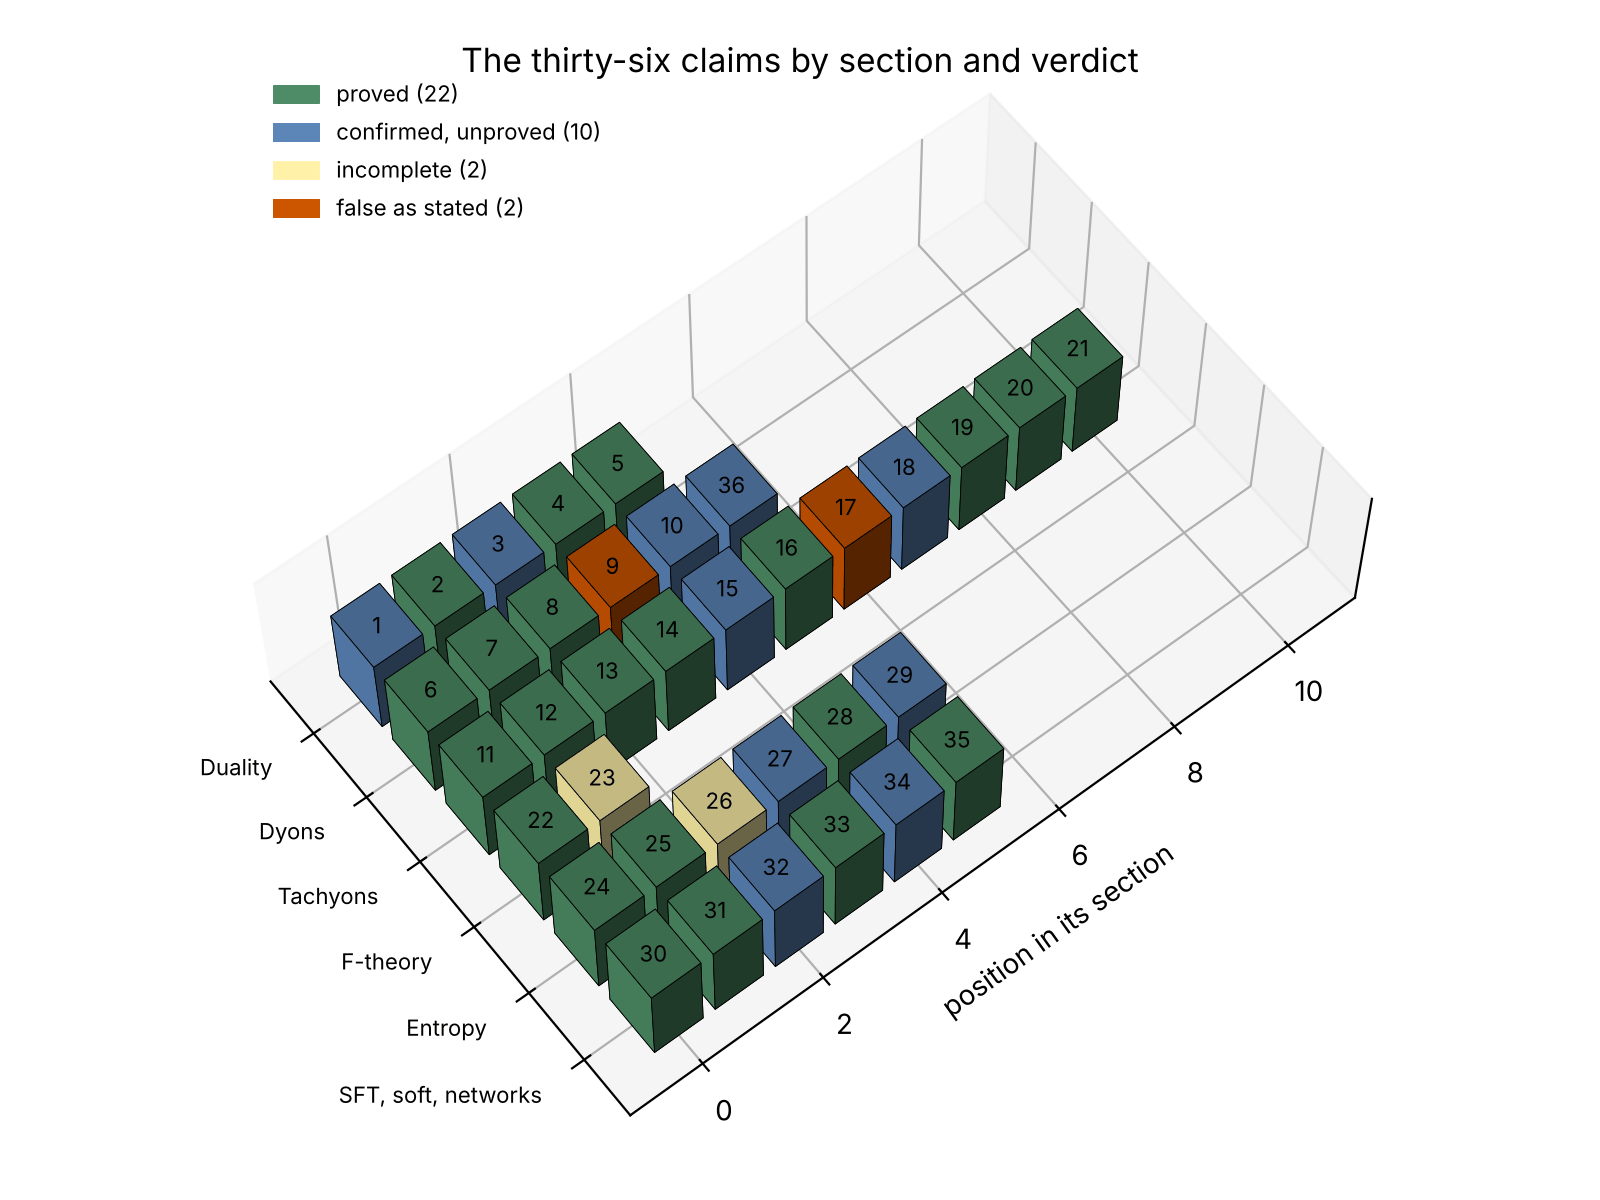
\includegraphics[width=\columnwidth]{figures/fig_verdicts.png}
\caption{The thirty-six claims of Tables~\ref{tab:catalogue} and~\ref{tab:catalogue2}, one block per claim, grouped by the section of the paper that treats them and coloured by verdict: proved, confirmed without proof, incomplete, false as stated. The two failures are claims 9 and 17; the two incomplete claims are 23 and 26.}
\label{fig:verdicts}
\end{figure}

\section{Duality and the monopole conjectures}\label{sec:sduality}

\subsection{The $SL(2,\ZZ)$ conjecture}\label{ssec:sl2z}

The conjecture of \cite{Sen94duality} (claim 1 of Table~\ref{tab:catalogue}) states that the heterotic string compactified on $T^6$, whose low energy theory is $\mathcal N=4$ supergravity coupled to 22 vector multiplets, is invariant under the group $SL(2,\ZZ)$ generated by the shift of the axion and by the inversion $\lambda\mapsto -1/\lambda$ of the complex coupling $\lambda = a + i e^{-\phi}$, acting on the electric and magnetic charge vectors $(Q,P)$ of the $O(6,22)$ lattice by the same matrix.\footnote{The conjecture was made in two steps. Schwarz and Sen \cite{SchwarzSen93} showed that the equations of motion of the low energy theory, not its action, are invariant under $SL(2,\RR)$, and that the charge lattice reduces the symmetry to $SL(2,\ZZ)$; \cite{Sen94duality} then proposed that the full string theory, at every order and beyond perturbation theory, has this symmetry. The $SL(2,\RR)$ of the equations of motion is a theorem of the supergravity theory; it is the lift to the full string theory that is the conjecture.} The inversion exchanges weak and strong coupling, so no perturbative computation can test it directly. Sen reduced the test to the spectrum of states that saturate the Bogomolnyi bound, whose masses and degeneracies are protected by supersymmetry: the conjecture requires that for every pair of coprime integers $(p,q)$ there exist states carrying $p$ units of electric and $q$ units of magnetic charge, in the same supermultiplet as the elementary string states with $(1,0)$.

For $q=1$ these are the dyons of the $\mathcal N=4$ theory and they were known to exist \cite{Osborn79}. For $(p,q) = (1,2)$ the conjecture requires a bound state of two monopoles and one unit of electric charge, and nothing in the classical theory produces such a state: the static BPS monopoles have no net force, but a normalisable quantum bound state is not supplied by a static separated configuration and there is no classical bound state. The prediction is therefore a genuine one, and it was tested in \cite{Sen94dyon}, as described in the next subsection. The subsequent tests of the conjecture are the three-string junction states \cite{Sen98network,Sen07junction}, the counting of quarter-BPS dyons (Section~\ref{sec:dyons}), whose partition function is a Siegel form invariant under the duality group, the match of the black hole entropy with the index (Section~\ref{sec:entropy}), and the equivalent statement for $\mathcal N=4$ super-Yang--Mills theory, where the conjecture of Montonen and Olive \cite{MontonenOlive77} is tested by the same bound states \cite{Sen94dyon,Porrati96,GauntlettLowe96,LeeWeinbergYi96}, by the modular properties of partition functions on four-manifolds \cite{VafaWitten94}, and by its embedding into the geometric Langlands programme \cite{KapustinWitten07}.

\begin{verdict}[claim 1]\label{ver:sl2z}
Confirmed. Every protected quantity that has been computed is consistent with the $SL(2,\ZZ)$ symmetry, and the strongest test, the exact dyon index of Section~\ref{sec:dyons}, is a Siegel form of the duality group. A general nonperturbative proof is not supplied here; which has no definition at strong coupling other than through such dualities; what a proof would require is a non-perturbative definition of the heterotic string on $T^6$, and none exists. The tests cited here do not constitute such a construction.
\end{verdict}

One point about the statement itself should be made precisely, because it is the kind of place where a conjecture can be ``wrong'' without its author being wrong. For gauge theories with a non-simply-laced gauge group the duality group of the $\mathcal N=4$ theory is not $SL(2,\ZZ)$: the inversion maps the gauge group $G$ to its Langlands dual $G^\vee$, and the group generated by the shift and the inversion is a Hecke group $\Gamma_0(q)$-type subgroup, with $q=2$ or $3$ \cite{GGPZ95,DFHK96,AKS06}. This is not a correction of \cite{Sen94duality} or of \cite{Sen94dyon}: both papers treat $SU(2)$ and the heterotic string, where the duality group is $SL(2,\ZZ)$, and \cite{Sen94dyon} is explicit that the test is for $SU(2)$. We mention it because the literature sometimes attributes an $SL(2,\ZZ)$ conjecture ``for all groups'' to the 1994 papers; they contain no such statement.

\subsection{The two-monopole bound state}\label{ssec:twomonopole}

The moduli space of two $SU(2)$ monopoles of total charge two is $\RR^3\times (S^1\times \mathcal M_0)/\ZZ_2$, where $\mathcal M_0$ is the Atiyah--Hitchin manifold \cite{AtiyahHitchin88}, a complete hyperk\"ahler four-manifold with an $SO(3)$ action and a metric known in closed form (for the hypercomplex structures underlying such metrics see also \cite{Bha22b}). The low energy dynamics of two monopoles is the supersymmetric quantum mechanics on this moduli space, and a bound state of two monopoles with one unit of electric charge and the right supermultiplet structure exists if and only if the Atiyah--Hitchin manifold carries a harmonic two-form that is square integrable, anti-self-dual (with the orientation fixed by the complex structures), odd under the $\ZZ_2$, and unique.\footnote{The electric charge of the state is the momentum along the $S^1$ factor, and the $\ZZ_2$ acts on it; the state with one unit of electric charge requires the form on $\mathcal M_0$ to be odd under the $\ZZ_2$ which combines with the half shift on $S^1$. The multiplet structure is fixed by the fermion zero modes: the state must be a single short multiplet of $\mathcal N=4$, which is the statement that the harmonic form is unique and of a definite duality type. Sen's paper carries this out in detail and we do not repeat it.} Sen wrote down the form. In the coordinates of \cite{AtiyahHitchin88}, with the metric $ds^2 = f^2 d\rho^2 + a^2\sigma_1^2 + b^2\sigma_2^2 + c^2\sigma_3^2$ on left-invariant forms with $d\sigma_i = \tfrac12\epsilon_{ijk}\sigma_j\wedge\sigma_k$, the form is
\begin{equation}\label{eq:senform}
\begin{aligned}
\omega &= F(\rho)\,\Big(d\sigma_1 - \frac{fa}{bc}\, d\rho\wedge\sigma_1\Big),\\
F(\rho) &= F_0\exp\Big(-\int_{\pi}^{\rho}\frac{fa}{bc}\,d\rho'\Big),
\end{aligned}
\end{equation}
which is anti-self-dual by the choice of the coefficient of $d\rho\wedge\sigma_1$, closed because $dF/d\rho = -(fa/bc)F$, and square integrable because $fa/(bc)\to\tfrac12$ as $\rho\to\infty$ (where $f\simeq -1$, $a\simeq b\simeq\rho$, $c\simeq -2$) makes $F$ decay as $e^{-\rho/2}$ while the volume grows polynomially; near the bolt $\rho\to\pi$, in the coordinates adapted to it, the form is smooth.\footnote{Equations (16) to (19) of \cite{Sen94dyon}. The form is invariant under the identification $(\rho,\theta,\phi,\psi)\sim(\rho,\pi-\theta,\pi+\phi,-\psi)$ that defines the Atiyah--Hitchin manifold and changes sign under $\psi\mapsto\psi+\pi$, which is the $\ZZ_2$ of the two-monopole moduli space; this is the parity required for odd electric charge. The uniqueness of the form among $L^2$ harmonic two-forms was argued in \cite{Sen94dyon} from the symmetries; the complete statement that the space of $L^2$ harmonic forms of $\mathcal M_0$ is one-dimensional is Hitchin's theorem below. Sen notes that the same form had appeared in work of Gibbons and Ruback for another purpose.}

\begin{theorem}[Sen 1994; Hitchin 2000]\label{thm:atiyahhitchin}
The space of $L^2$ harmonic forms on the Atiyah--Hitchin manifold is one-dimensional. It is spanned by the two-form \eqref{eq:senform}, which is anti-self-dual and odd under the $\ZZ_2$ that acts on the moduli space of two monopoles.
\end{theorem}

\begin{proof}
Existence, anti-self-duality, square integrability and the $\ZZ_2$ parity are the computation of \cite{Sen94dyon} summarised above; we have checked each step. The uniqueness result is taken from \cite{Hitchin00}. We do not infer it merely by counting a circle fixed set: orientation and the particular cover of the monopole moduli space matter.
\end{proof}

\begin{verdict}[claim 2]
Proved. The bound state predicted by $SL(2,\ZZ)$ exists, and it is the only one in the two-monopole sector, which is also what the duality predicts: the $(1,2)$ state must be a single short multiplet.
\end{verdict}

\subsection{The Sen conjecture on $L^2$ cohomology}\label{ssec:senconjecture}

The argument of \cite{Sen94dyon} applies to any charge. Let $\mathcal M_k^0$ denote the reduced moduli space of $k$ monopoles, of real dimension $4k-4$, and let $\mathcal M_k = \RR^3\times(S^1\times\mathcal M^0_k)/\ZZ_k$. The states with $k$ units of magnetic charge and $p$ units of electric charge, with $\gcd(p,k)=1$, correspond to $L^2$ harmonic forms on $\mathcal M^0_k$ transforming under the $\ZZ_k$ by $e^{2\pi i p/k}$; $S$-duality requires exactly one such form, in the middle degree $2k-2$, for every $p$ coprime to $k$, and none for other $p$ (which would give states not in the duality orbit of the elementary string states). This is the \emph{Sen conjecture}; Segal and Selby \cite{SegalSelby96} proved that the image of the compactly supported cohomology in the ordinary cohomology, which is a lower bound for the $L^2$ cohomology, has exactly the predicted dimension in the middle degree and vanishes elsewhere. The conjecture is thus reduced to the statement that every $L^2$ harmonic form comes from compactly supported cohomology.

\begin{theorem}[published partial results and their hypotheses]\label{thm:senconj}
The Segal--Selby image has the dimensions predicted by the conjecture \cite{SegalSelby96}. Hitchin's middle-degree result and the charge-two case are established in \cite{Hitchin00}. Fritzsch--Kottke--Singer \cite[Theorem~1.2 and Section~6]{FKS18} state the coprime electric/magnetic charge case for arbitrary magnetic charge, using their metric compactification. Their introduction announces a separate complete proof of the asymptotic metric description. Kottke--Rochon \cite[Theorem~A]{KottkeRochon24} give the charge-three result provided the monopole metric has the announced quasi-fibered boundary structure. These hypotheses and dependencies are part of the statements, not additional results proved here.
\end{theorem}
\begin{proof}
This paragraph records the cited results with their own hypotheses. In particular it does not reduce all progress for $k\ge4$ to a lower bound from compactly supported cohomology: the coprime case is explicitly treated in Section~6 of \cite{FKS18}. Conversely, quoting Theorem~A of \cite{KottkeRochon24} without its metric qualification would overstate that theorem.
\end{proof}
\begin{verdict}[claim 3]
Supported, with substantial established and conditional cases. No proof of the complete statement in every character is given here. The non-coprime sector and the cited metric construction dependencies must be checked separately before asserting a general unconditional closure. These are mathematical questions rather than evidence that the original conjecture is false.
\end{verdict}

\subsection{Duality-symmetric actions, the Kerr--Sen black hole and string networks}\label{ssec:misc}

Three further claims of this period are theorems and we record them briefly.

\begin{proposition}[claims 4, 5 and 35]\label{prop:misc}
\begin{enumerate}[leftmargin=1.6em,itemsep=1pt]
\item[(i)] Schwarz and Sen \cite{SchwarzSen94} wrote an action with two gauge potentials and a first-order Lagrangian; it is invariant under the duality rotation and has equations of motion equivalent to Maxwell's equations; the same construction gives a duality-symmetric form of the heterotic effective action in four dimensions.
\item[(ii)] The metric, dilaton, gauge field and axion of \cite{Sen92kerr} solve the equations of motion of the low energy heterotic string in four dimensions; the solution is obtained from the Kerr solution by the $O(1,1)$ twisting transformation of the string background, which maps solutions to solutions.
\item[(iii)] A planar network of $(p,q)$-strings of type IIB with the charges conserved at each junction and the angles fixed by the tensions is supersymmetric, preserving one quarter of the supersymmetry. The proof is in \cite{Sen98network} itself, from the supersymmetry algebra of the $(p,q)$-string; the three-string junction was shown to be a BPS state by \cite{ReyYee98} and, lifted to a holomorphic membrane in M-theory, by \cite{MatsuoOkuyama98}. The statement was a theorem when it was made, and the catalogue records it as proved.
\end{enumerate}
\end{proposition}

\begin{proof}
(i) is a direct computation in the cited paper: the two potentials $A^{(1)}, A^{(2)}$ enter through a first-order Lagrangian whose equations of motion are $F^{(2)} = *F^{(1)}$ up to gauge, so that eliminating $A^{(2)}$ recovers the Maxwell equations; the Lorentz invariance is not manifest but is verified. (ii) is the statement that the twisting transformation of \cite{Sen92kerr}, which acts on backgrounds with a Killing direction, is a symmetry of the equations of motion; this was proved for the full string effective action at lowest order in $\alpha'$, and the Kerr--Sen metric is the image of Kerr. (iii) follows from the supersymmetry algebra: the BPS condition for a network is linear in the charge vectors at each junction, and the tension balance at a junction is the statement that the central charges add; \cite{Sen98network} verifies this and \cite{Sen07junction} uses the same networks to count quarter-BPS dyons. For (iii), ``proved'' refers to the effective BPS configuration; existence and completeness of the quantum spectrum at finite coupling are separate physical questions.
\end{proof}

\section{Quarter-BPS dyons}\label{sec:dyons}

\subsection{The partition function and its product formula}\label{ssec:chl}

Dijkgraaf, Verlinde and Verlinde \cite{DVV97} proposed that the index of quarter-BPS dyons of the heterotic string on $T^6$, with electric charge $Q$ and magnetic charge $P$ in the lattice $\Gamma^{6,22}$, is a Fourier coefficient of the inverse of the Igusa cusp form $\Phi_{10}$ of weight ten on $Sp(2,\ZZ)$:
\begin{equation}\label{eq:dvv}
d(Q,P) = (-1)^{Q\cdot P+1}\oint_{\mathcal C} d\rho\,d\sigma\,dv\; \frac{e^{-\pi i(\rho Q^2 + \sigma P^2 + 2 v\, Q\cdot P)}}{\Phi_{10}(\rho,\sigma,v)} ,
\end{equation}
the contour $\mathcal C$ being a three-torus at fixed, large imaginary parts of $(\rho,\sigma,v)$, with the sign of $\operatorname{Im} v$ determined by the asymptotic moduli \cite{Sen07walls}.\footnote{The sign $(-1)^{Q\cdot P+1}$ converts the Fourier coefficient into the helicity trace index $B_6$ of the four-dimensional theory; it was identified in \cite{Sen07walls,Sen07twocentred} (footnote 2 of \cite{Sen07twocentred} records that it was absent from the earlier papers) and traced to the change of statistics between the five- and four-dimensional descriptions in the presence of a Kaluza--Klein monopole. The index $d$ of this paper is $-B_6$ in the notation of \cite{Sen11positivity}.} Jatkar and Sen \cite{JatkarSen06} proposed the analogous formula for the CHL orbifolds $\ZZ_N$, $N=2,3,5,7$, with $\Phi_{10}$ replaced by a Siegel form $\Phi_k$ of weight $k = 24/(N+1)-2$ for a subgroup of $Sp(2,\ZZ)$, and David, Jatkar and Sen \cite{DJS06,DJS07} derived the product representation
\begin{equation}\label{eq:product}
\begin{split}
\Phit(\rho,\sigma,v) ={}& e^{2\pi i(\rho + \sigma/N + v)}\prod_{b=0}^{1}\prod_{r=0}^{N-1}\prod_{\substack{k'\in\ZZ+r/N,\ l\in\ZZ,\ j\in 2\ZZ+b\\ k',l\ge 0;\ j<0 \text{ if } k'=l=0}}\big(1 - e^{2\pi i(k'\sigma + l\rho + jv)}\big)^{c(k',l,j)},\\
c(k',l,j) ={}& \sum_{s=0}^{N-1} e^{2\pi i s l/N} c^{(r,s)}_b(4k'l-j^2),
\end{split}
\end{equation}
from the twisted elliptic genera
\[
F^{(r,s)}(\tau,z) = \sum_b\sum_{j\in 2\ZZ+b}\sum_{n\in\ZZ/N} c^{(r,s)}_b(4n-j^2)\, q^n y^j
\]
of K3, by the method of \cite{DVV97}: the dyons are counted in the type IIB frame on $K3\times T^2$ by the D1--D5 system bound to a Kaluza--Klein monopole, and the three factors of the partition function (the motion of the centre of mass, the Kaluza--Klein monopole and the D1--D5 world-volume theory) each contribute a product. For $N=1$, \eqref{eq:product} with the K3 elliptic genus $8A(\tau,z)$ is the Borcherds product for $\Phi_{10}$.

\begin{theorem}[claim 6]\label{thm:chl}
For $N\in\{2,3,5,7\}$ the function $\Phit_k$ defined by \eqref{eq:product} is a Siegel modular form of weight $k$ for the subgroup $\widetilde G\subset Sp(2,\ZZ)$ of \cite{JatkarSen06}, and it coincides with the form constructed by Borcherds lifting in \cite{DabholkarNampuri07} and with the genus-two partition function of \cite{DabholkarGaiotto07}.
\end{theorem}

\begin{proof}
The modularity of the product and its identification with the additive lift are \cite[Section~3]{DabholkarNampuri07}, who show that \eqref{eq:product} is the Borcherds lift of the twisted elliptic genus and that the lift is the Siegel form of \cite{JatkarSen06}; the identification with the genus-two partition function of the heterotic string is \cite{DabholkarGaiotto07}. For $N=1$ the product is the classical Borcherds product of $\Phi_{10}$ \cite{GritsenkoNikulin97}. We have checked \eqref{eq:product} numerically for $N=1,2$ by reproducing the tables of \cite{Sen11positivity}, see Appendix~\ref{app:computation}.
\end{proof}

The physical content of the conjecture, that this Siegel form counts the quarter-BPS states of the string theory, is not a theorem and cannot be: it is a statement about the strong coupling regime, tested through the duality orbit. The tests are the agreement with the black hole entropy to the first two orders in the large charge expansion \cite{CDKM04,JatkarSen06,DavidSen06} and at the logarithmic order (Section~\ref{sec:quantum}), the wall-crossing behaviour described next, and the agreement at low charges with the string-junction counting \cite{Sen07junction}.

\subsection{Walls of marginal stability and the two-centred states}\label{ssec:walls}

The Fourier coefficient \eqref{eq:dvv} depends on the contour because $1/\Phit$ has double poles on the divisors $v=0$ and its images under the duality group. Sen \cite{Sen07walls} identified the poles with the walls of marginal stability of the quarter-BPS dyon, on which it can decay into a pair of half-BPS states with charges $(Q,0)$ and $(0,P)$ (and the images under duality), and computed the jump of the index across the wall $v=0$ from the residue of the double pole. Near $v=0$,
\begin{equation}\label{eq:nearpole}
\Phit(\rho,\sigma,v) = -4\pi^2 v^2 f(N\rho)\,g(\sigma/N) + O(v^4),
\end{equation}
with $f(\tau)^{-1}$ and $g(\tau)^{-1}$ the generating functions of the half-BPS electric and magnetic states; for $N=1$, $f=g=\eta^{24}$ and $d_h(Q) := $ coefficient of $q^{Q^2/2}$ in $\eta(\tau)^{-24}=q^{-1}\prod_{m\ge1}(1-q^m)^{-24}$, so that $d_h = 1, 24, 324, 3200, 25650, \dots$ for $Q^2/2 = -1,0,1,2,3,\dots$.

\begin{theorem}[claim 7; Sen 2007]\label{thm:wallcrossing}
Let $N=1$ and let $d_{>}(Q,P)$, $d_{<}(Q,P)$ denote the Fourier coefficients of \eqref{eq:dvv} without the sign $(-1)^{Q\cdot P+1}$, taken over the contours with $\operatorname{Im}v<0$ and $\operatorname{Im}v>0$ respectively. Then
\begin{equation}\label{eq:jump}
d_{>}(Q,P) - d_{<}(Q,P) = -\,Q\cdot P\; d_h(Q)\, d_h(P).
\end{equation}
In particular the index $d = (-1)^{Q\cdot P+1}d_{\gtrless}$ changes across the wall by $(-1)^{Q\cdot P}\,Q\cdot P\,d_h(Q)d_h(P)$, whose absolute value $|Q\cdot P|\,d_h(Q)d_h(P)$ is the index of a two-centred configuration of a half-BPS electric and a half-BPS magnetic centre with angular momentum $(|Q\cdot P|-1)/2$.
\end{theorem}

\begin{proof}
The difference of the two contour integrals is the residue at $v=0$. From \eqref{eq:nearpole},
\[
1/\Phit = -(4\pi^2v^2)^{-1}f(\rho)^{-1}g(\sigma)^{-1}\bigl(1+O(v^2)\bigr),
\]
and the residue of $e^{-2\pi i v Q\cdot P}v^{-2}$ at $v=0$ is $-2\pi i\,Q\cdot P$; the remaining integrals over $\rho$ and $\sigma$ pick out $d_h(Q)$ and $d_h(P)$, and the factors of $2\pi i$ cancel against the normalisation of the contour. This is \cite[eq.~(2.13)]{Sen07twocentred}. The sign and the factor $|Q\cdot P|$ are those of a bound state of two centres carrying angular momentum $J = (|Q\cdot P|-1)/2$ from the electromagnetic field, with $2J+1 = |Q\cdot P|$ states \cite{Sen07twocentred,DenefMoore11}.

We have also verified \eqref{eq:jump} independently of the residue computation, by expanding the product \eqref{eq:product} for $N=1$ in exact arithmetic on both sides of the wall and comparing the coefficients: for every $Q^2,P^2\in\{2,4,6\}$ and $|Q\cdot P|\le 4$ the two expansions differ by exactly $-Q\cdot P\,d_h(Q)d_h(P)$ (Appendix~\ref{app:computation}, Table~\ref{tab:phi10}).
\end{proof}

\begin{verdict}[claim 7]
Proved. The formula is a residue computation, and the identification of the jump with the two-centred bound state is confirmed by the exact match of the degeneracy $|Q\cdot P|d_h(Q)d_h(P)$ with the quantisation of the two-centred solution \cite{Sen07twocentred}, and by the general wall-crossing formulas of Denef and Moore \cite{DenefMoore11} and of Kontsevich and Soibelman \cite{KS11}, of which \eqref{eq:jump} is the primitive case.
\end{verdict}

\subsection{Negative discriminant states}\label{ssec:negative}

The discriminant $\Delta=Q^2P^2-(Q\cdot P)^2$ must be positive for the regular classical single-centred solutions in the stated sector. The treatment of negative discriminant states uses chamber-dependent sums over two-centred decompositions and bound-state metamorphosis \cite{Sen11negative,CKMRW20}. A single primitive contribution has the form
\begin{equation}\label{eq:negative}
(-1)^{\langle\Gamma_1,\Gamma_2\rangle+1}|\langle\Gamma_1,\Gamma_2\rangle|\,d_h(\Gamma_1)d_h(\Gamma_2).
\end{equation}
The full answer requires the allowed decompositions and their identifications. For example $(Q^2,P^2,Q\cdot P)=(2,2,-2)$ has $\Delta=0$, not negative discriminant; it must not be used as a negative-discriminant example. The identity $209952-648=209304$ is an arithmetic wall-crossing check, not a proof of a proposed microscopic decomposition. Similarly $327=3\cdot109$ does not identify $109$ as a half-BPS degeneracy.

\begin{theorem}[claim 8]\label{thm:negative}
Every Fourier coefficient of $1/\Phi_{10}$ with negative discriminant is given by a finite sum of two-centred contributions of the form \eqref{eq:negative} over the duality images of the charges. The CHL generalisations require the separate hypotheses and formulas of \cite{Sen11negative}; no CHL formula is deduced solely from the $\Phi_{10}$ theorem.
\end{theorem}

\begin{proof}
For $\Phi_{10}$ this is the main theorem of Chowdhury, Kidambi, Murthy, Reys and Wrase \cite{CKMRW20}, who derive the exact formula for all polar (negative discriminant) coefficients from the mock modular decomposition of \cite{DMZ12} and check it against $1650$ coefficients; its direct scope is the $K3\times T^2$ theory associated with $\Phi_{10}$, and it is not cited as a proof for every CHL form. The physical interpretation, that the states are two-centred, is \cite{Sen11negative}.
\end{proof}

\section{The positivity conjecture}\label{sec:positivity}

\subsection{The statement and its hypothesis}\label{ssec:positivitystatement}

A single-centred supersymmetric black hole in four dimensions has a spherically symmetric horizon and carries no angular momentum. The helicity trace index $B_6$ of a quarter-BPS state is $-\frac{1}{6!}\Tr\big[(-1)^{2h}(2h)^6\big]$, and for a configuration whose only degrees of freedom beyond the horizon are the twelve fermion zero modes of the broken supersymmetries, the trace evaluates to $-1$ times the number of horizon states; the sign is fixed and the index is negative, that is, $d = -B_6 > 0$. Sen \cite{Sen11positivity} turned this into a conjecture about Fourier coefficients. In the region $\mathcal R$ of the axion--dilaton moduli space in which the attractor point of the charges $(Q,P)$ lies, bounded by walls of marginal stability, the intended contribution is isolated under the exclusions described in the original argument, and the Fourier coefficient \eqref{eq:dvv} taken with the contour of that region should be positive. For the heterotic string on $T^6$ the region is cut out by
\begin{equation}\label{eq:senconditions}
\begin{gathered}
Q\cdot P\ge 0,\qquad Q\cdot P\le Q^2,\qquad Q\cdot P\le P^2,\\
Q^2>0,\qquad P^2>0,\qquad Q^2P^2-(Q\cdot P)^2>0,
\end{gathered}
\end{equation}
(equation (3.7) of \cite{Sen11positivity}), and for the $\ZZ_2$ CHL model, whose duality group is $\Gamma_1(2)$, by
\begin{equation}\label{eq:z2conditions}
\begin{gathered}
Q^2>0,\qquad P^2>0,\qquad Q^2P^2>(Q\cdot P)^2,\\
2Q^2+P^2\ge 3(Q\cdot P),\qquad 2Q^2\ge Q\cdot P,\\
P^2\ge Q\cdot P,\qquad Q\cdot P\ge 0
\end{gathered}
\end{equation}
(equation (3.9) there, with $Q^2$ normalised so that $NQ^2/2\in\ZZ$). The fourth condition is linear in $Q\cdot P$: it is the image of the wall $Q\cdot P\ge0$ under the second matrix of Sen's equation (3.8), $(Q,P)\mapsto(-Q+P,-2Q+P)$, whose inner product is $2Q^2-3\,Q\cdot P+P^2$. Equations (3.25) and (4.7) of \cite{CD19} print it as $2Q^2+P^2-3(Q\cdot P)^2\ge0$; that squared form is a misprint of the same condition, and it would exclude, for instance, the triple $(Q^2,P^2,Q\cdot P)=(3,2,2)$ of Table~\ref{tab:violations}. Sen verified the positivity of $d(Q,P)$ on these cones for the heterotic string and for the CHL models $N=2,3,5,7$ in the range of charges of his Tables~1 to~5, and stated the conjecture for all charges in the cone. We have reproduced his Tables~1 and~2 exactly (Appendix~\ref{app:computation}).

The hypothesis of the argument is explicit in \cite{Sen11positivity}: the conclusion requires ``some duality frame in which only single centered black hole solution, whose only hair are the fermion zero modes associated with broken supersymmetry, contributes'' to the index. In the heterotic frame the quarter-BPS black hole does have hair beyond the fermion zero modes (the hair modes identified in \cite{BMS09hair}), but there is a frame, the type IIB frame on $K3\times T^2$, in which the hair reduces to the fermion zero modes; this is what makes the conjecture consistent there, and it is in this frame that it was later proved for the first two magnetic charges.

\begin{theorem}[Bringmann--Murthy]\label{thm:bringmannmurthy}
For type II string theory on $K3\times T^2$, equivalently the heterotic string on $T^6$ with the form $1/\Phi_{10}$, the single-centred index $d^*(Q,P)$ is positive for every charge with $P^2\in\{2,4\}$ and $Q^2P^2-(Q\cdot P)^2>0$, and for every charge in the $SL(2,\ZZ)$ orbit of such a charge. For type II string theory on $T^6$ the index of every single-centred one-eighth BPS black hole is positive.
\end{theorem}

\begin{proof}
Write $m=P^2/2$, $n=Q^2/2$, $\ell=Q\cdot P$, and let $\psi^F_m=\sum c^F_m(n,\ell)q^n\zeta^\ell$ be the finite part of the Fourier--Jacobi coefficient $\psi_m$ of $1/\Phi_{10}$, the difference between $\psi_m$ and its Appell--Lerch polar part. Bringmann and Murthy prove $(-1)^{\ell+1}c^F_m(n,\ell)>0$ for $m\in\{1,2\}$ and $4mn-\ell^2>0$ \cite[(3.8) and Sections~4--6]{BringmannMurthy13}, and the positivity of the one-eighth BPS indices, which are coefficients of $\theta_1(\tau,z)^2/\eta(\tau)^6$ \cite[case (1a)]{BringmannMurthy13}. That $(-1)^{\ell+1}c^F_m(n,\ell)$ is the single-centred index of the charge is the theorem of Bhand, Sen and Singh \cite[Theorem~5.4(a)]{BSS25} with $N=1$, whose set $A_1$ \cite[(5.64)]{BSS25} contains every charge with $4mn-\ell^2\ge m^2$, $m$ being the index of the form; for $m\le 2$ this holds whenever $4mn-\ell^2>0$. The single-centred index is invariant under $SL(2,\ZZ)$ \cite[Section~5.3]{BSS25}, which gives the statement on orbits.
\end{proof}

The proof of \cite{BringmannMurthy13} is written for each index separately, and the cases $P^2\ge 6$ are not covered by it.

\subsection{The \texorpdfstring{$\ZZ_2$}{Z2} CHL model at \texorpdfstring{$P^2=2$}{P2=2}}\label{ssec:chlpositivity}

For the CHL models the decomposition into polar and finite parts is \cite{BSS25}.\footnote{Throughout, $d^*(Q,P)$ is the coefficient that \cite[Theorem~5.4]{BSS25} identifies with the single-centred index: $(-1)^{\ell+1}$ times a Fourier coefficient of a finite part. The positivity theorems are statements about these coefficients; reading them as counts of single-centred black hole states rests on the physical input of \cite{Sen11positivity,BSS25}. The decomposition is due to \cite{BSS25}, and at $P^2=2$ the reduction of $\psi_1$ to Eisenstein series and class numbers to \cite{CD19}; what is proved here is the sign of every coefficient and the reduction of every orbit to one coefficient.} We use it to prove positivity at the first magnetic charge of the $\ZZ_2$ model. Write $q=e^{2\pi i\tau}$, $\zeta=e^{2\pi iz}$, let $A$, $B$ and the weight-two form $E_2(\tau)=2E(2\tau)-E(\tau)=1+24\sum_{n\ge1}\sigma_{\rm odd}(n)q^n$ of $\Gamma_0(2)$ be as in \eqref{eq:tor2genera}, let $E_4=1+240\sum\sigma_3(n)q^n$, $g(\tau)=\eta(\tau)^8\eta(2\tau)^8$, and let
\[
\mathcal H(\tau,z)=\sum_{n\ge0}\sum_{r\in\ZZ}H(4n-r^2)\,q^n\zeta^r
\]
be the generating function of the Hurwitz class numbers, with $H(0)=-\tfrac1{12}$ and $H(N)=0$ for $N<0$. Let $\psi_1$ be the Fourier--Jacobi coefficient of $1/\Phit_6$ at $P^2=2$, in the normalisation of \cite{BSS25}, in which $q$ carries $Q^2$ and $\zeta$ carries $Q\cdot P$.

\begin{theorem}\label{thm:chlpositivity}
In the $\ZZ_2$ CHL model the single-centred index $d^*(Q,P)$ is positive for every charge with $P^2=2$ and $Q^2P^2>(Q\cdot P)^2$, and for every charge in the $\Gamma_1(2)$ orbit of such a charge.
\end{theorem}

The proof occupies the rest of this subsection. Its first two steps identify the generating function, the remaining ones prove the signs.

\paragraphx{Step 1: the single-centred index.} Bhand, Sen and Singh \cite[(5.45)]{BSS25} give the polar part
\begin{equation}\label{eq:chlpolar}
\psi_1^P(\tau,z)=\frac{52}{g(\tau)}\sum_{s\in\ZZ}\frac{q^{2(s^2+s)}\zeta^{2s+1}}{(1-q^{2s}\zeta)^2},
\end{equation}
where $52$ is the coefficient of $p^{1/2}$ in $1/g(\sigma/2)$, $p=e^{2\pi i\sigma}$, namely $\binom92+8+8$. Write $\psi_1^F=\psi_1-\psi_1^P=\sum c^F(m,\ell)q^m\zeta^\ell$. By \cite[Theorem~5.4(b)]{BSS25}, for a charge with $Q^2=m$, $P^2=2$, $Q\cdot P=\ell$ in their set $B$, $d^*=\tfrac12(-1)^{\ell+1}c^F(m,\ell)$. Their set $B_1$ \cite[(5.65)]{BSS25} at $N=2$ and $P^2/2=1$ is the condition $2m-\ell^2\ge\tfrac14$, which for integers is $Q^2P^2-(Q\cdot P)^2=2m-\ell^2>0$. The theorem is therefore the statement $(-1)^{\ell+1}c^F(m,\ell)>0$ for $2m-\ell^2>0$; the orbits follow from the $\Gamma_1(2)$ invariance of $d^*$.

\paragraphx{Step 2: the finite part in closed form.} Chattopadhyaya and David \cite[(3.12)--(3.22)]{CD19} reduce $\psi_1$ to the forms $A$, $B$, $E_2$, $E_4$ through the twisted elliptic genera of the model, separate the double pole with the identity $\phi_{0,1}^2/\phi_{-2,1}=144\sum_s q^{s^2+s}\zeta^{2s+1}(1-q^s\zeta)^{-2}+E_4\phi_{-2,1}-288\,\mathcal H$ for the weak Jacobi forms $\phi_{0,1}=4A$, $\phi_{-2,1}=-B$ \cite[Section~3]{BringmannMurthy13}, taken at $2\tau$, and find
\begin{equation}\label{eq:chlclosed}
g\,\psi_1^F=-\tfrac{20}{9}\,A(2\tau,z)\,E_2(\tau)-B(2\tau,z)\big(\tfrac4{45}E_4(\tau)+\tfrac7{15}E_4(2\tau)\big)-104\,\mathcal H(2\tau,z).
\end{equation}
This is their (3.22) after the relation $E_4(2\tau)=-\tfrac14E_4(\tau)+\tfrac54E_2(\tau)^2$ of their (3.21). In the printed (3.22) the factor of $A(2\tau,z)$ is $E_2(2\tau)$; it is $E_2(\tau)$, as in the line before it; with $E_2(2\tau)$ the coefficient of $\zeta$ in $\psi^F_1$ would be $\tfrac{64}{3}$ instead of $8$. We checked \eqref{eq:chlpolar} and \eqref{eq:chlclosed} against the product formula \eqref{eq:product} in exact arithmetic for $Q^2\le28$, $|Q\cdot P|\le7$ \cite{Bha26}.

The identity $4\theta_4(\tau,z)^2/\theta_4(\tau)^2=\tfrac43A(\tau,z)+\tfrac13B(\tau,z)E_2(\tau/2)$ \cite[(3.14)]{CD19}, taken at $2\tau$, gives $A(2\tau,z)=3T-\tfrac14B(2\tau,z)E_2(\tau)$ with $T=\theta_4(2\tau,z)^2/\theta_4(2\tau)^2$, and $E_2(\tau)^2=\tfrac15\big(E_4(\tau)+4E_4(2\tau)\big)$. Substituting,
\begin{equation}\label{eq:chlclosed2}
g\,\psi_1^F=-\tfrac{20}3\,E_2(\tau)\,T+\tfrac{16}3\,M(\tau)\,B(2\tau,z)-104\,\mathcal H(2\tau,z),\qquad M=\frac{E_4(\tau)-E_4(2\tau)}{240}.
\end{equation}

\paragraphx{Step 3: theta components.} Put $x=q^{1/2}$. Each of $T$, $B(2\tau,z)$ and $\mathcal H(2\tau,z)$ is a sum $\sum_\ell q^{\ell^2/2}\zeta^\ell f_{\ell\bmod2}(x)$, and so is the right side of \eqref{eq:chlclosed2}; call its components $n_0$, $n_1$ and write $n_j=\sum_t n_j(t)x^t$, where $t\equiv j \pmod 2$. Then $\psi_1^F=\sum_\ell q^{\ell^2/2}\zeta^\ell h_{\ell\bmod 2}$ with $h_j=n_j/g$, and $c^F(m,\ell)$ is the coefficient of $x^{2m-\ell^2}$ in $h_{\ell\bmod2}$. Expanding the squares, with $\ell=a+b$ and $u=a-b$,
\[
\theta_4(2\tau,z)^2=\sum_\ell(-1)^\ell q^{\ell^2/2}\zeta^\ell\!\!\sum_{u\equiv\ell\,(2)}\!\!x^{u^2},\qquad
\theta_1(2\tau,z)^2=\sum_\ell(-1)^\ell q^{\ell^2/2}\zeta^\ell\!\!\sum_{u\not\equiv\ell\,(2)}\!\!x^{u^2},
\]
so that the combination $-f_0+f_1$ is $-\theta_3(x)/\theta_4(2\tau)^2$ for $T$ and $-\theta_3(x)/\eta(2\tau)^6$ for $B(2\tau,z)$, where $\theta_3(x)=\sum_{n\in\ZZ}x^{n^2}$. The components of $\mathcal H(2\tau,z)$ are $\sum_t H(t)x^t$ over $t\equiv j$. With $\theta_4(2\tau)=\eta(\tau)^2/\eta(2\tau)$, the numbers $u(t)$ defined by $u(t)=-n_0(t)-104H(t)$ for even $t$ and $u(t)=n_1(t)+104H(t)$ for odd $t$ are the coefficients of
\begin{equation}\label{eq:chlS}
\sum_{t\ge0}u(t)x^t=\frac{\theta_3(x)\,G}{\eta(2\tau)^6},\qquad G=\tfrac{20}3\,E_2(\tau)\frac{\eta(2\tau)^8}{\eta(\tau)^4}-\tfrac{16}3\,M(\tau).
\end{equation}

\paragraphx{Step 4: the form $G$.} As a function of $\tau/2$, $G$ is a modular form of weight four for $\Gamma_0(4)$, a space of dimension three with Sturm bound two. Comparing the coefficients of $x^0$, $x^1$, $x^2$,
\begin{equation}\label{eq:chlG}
G=\tfrac1{36}E_4(x)-\tfrac{49}{180}E_4(x^2)+\tfrac{11}{45}E_4(x^4)=\sum_{j\ge1}\gamma(j)x^j,
\end{equation}
where $E_4(x)=1+240\sum\sigma_3(j)x^j$. Since $\sigma_3(2^am)=\sigma_3(m)(8^{a+1}-1)/7$ for odd $m$, this gives $\gamma(j)=\tfrac{20}3\sigma_3(j)$ for odd $j$ and $\gamma(j)=-\tfrac{16}3\,8^{a-1}\sigma_3(m)$ for $j=2^am$, $a\ge1$, $m$ odd. Hence $\gamma(j)\ge\tfrac{20}3j^3$ for odd $j$, and $\gamma(j)\ge-\tfrac23\zeta(3)j^3$ for even $j$, because $8^{a-1}\sigma_3(m)=\tfrac18 j^3\,\sigma_3(m)/m^3$.

\paragraphx{Step 5: $\theta_3G$ has positive coefficients.} Let $\kappa(k)=\sum_{n\in\ZZ}\gamma(k-n^2)$, with $\gamma(j)=0$ for $j\le0$, be the coefficients of $\theta_3(x)G$. Put $f(y)=(k-y^2)^3$ for $|y|\le\sqrt k$ and $f=0$ otherwise. The integers $n$ with $k-n^2$ odd form one class modulo two, and those with $k-n^2$ even the other. For a function that increases and then decreases, a sum over a class of step two differs from half the integral by at most the maximum, here $k^3$; the integral of $f$ is $\tfrac{32}{35}k^{7/2}$. By Step~4,
\begin{equation}\label{eq:chlbound}
\kappa(k)\ \ge\ \tfrac{20}3\big(I-k^3\big)-\tfrac23\zeta(3)\big(I+k^3\big)=k^3\big(\lambda\sqrt k-\mu\big),\qquad I=\tfrac{16}{35}k^{7/2},
\end{equation}
with $\lambda=\tfrac{16}{35}\big(\tfrac{20}3-\tfrac23\zeta(3)\big)>2.681$ and $\mu=\tfrac{20}3+\tfrac23\zeta(3)<7.469$. The right side is positive for $k\ge8$, and $\kappa(1),\dots,\kappa(7)=\tfrac{20}{3},\,8,\,176,\,\tfrac{992}{3},\,768,\,1520,\,2368$ are positive. So $\kappa(k)>0$ for every $k\ge1$, and $\kappa(0)=0$.

\paragraphx{Step 6: the components.} The coefficients of $x/\eta(2\tau)^6=\prod(1-x^{4r})^{-6}$ are nonnegative with constant term one, so \eqref{eq:chlS} gives $u(t)\ge\kappa(t+1)>0$ for every $t\ge0$. Since $H(t)\ge0$ for $t>0$, $n_0(t)=-u(t)-104H(t)<0$ for even $t\ge2$, while $n_0(0)=-\tfrac{20}3+\tfrac{104}{12}=2$. For odd $t$, $n_1(t)=u(t)-104H(t)$. Here $H(1)=0$, and $H(t)\le t$ for $t\ge3$: a reduced form $(a,b,c)$ of discriminant $-t$ has $|b|\le a\le\sqrt{t/3}$ and is fixed by $(a,b)$, so $H(t)\le\sqrt{t/3}\,\big(2\sqrt{t/3}+1\big)\le t$. For $t\ge10$, \eqref{eq:chlbound} at $k=t+1\ge11$ gives $u(t)\ge k^3(\lambda\sqrt k-\mu)>104k>104H(t)$, and for $t\le9$ the inequality $n_1(t)>0$ is read off the values $n_1(1),n_1(3),\dots,n_1(9)=8,\ 296,\ 1568,\ 6040,\ 18472$. Thus every coefficient of $n_1$ is positive, and $-n_0=-2+\sum_{k\ge1}a_kq^k$ with $a_k=-n_0(2k)>0$.

\paragraphx{Step 7: division by $g$.} The function $1/g=q^{-1}\prod_r(1-q^r)^{-8}(1-q^{2r})^{-8}$ has positive coefficients, so $h_1=n_1/g$ does, and $c^F(m,\ell)>0$ for every odd $\ell$. For even $\ell$, write $\Pi=\prod_r(1-q^r)^{-8}(1-q^{2r})^{-8}=\sum p(m)q^m$. Its logarithmic derivative gives $m\,p(m)=\sum_{k=1}^m s(k)p(m-k)$ with $s(k)=8\sigma(k)+16\sigma(k/2)$. Suppose $a_k>2s(k)/k$ for every $k$. Then for $m\ge1$ the coefficient of $q^m$ in $(-2+\sum a_kq^k)\Pi$ is
\[
-2p(m)+\sum_{k=1}^ma_kp(m-k)\ >\ -2p(m)+\frac2m\sum_{k=1}^m s(k)p(m-k)=0,
\]
and $-h_0=q^{-1}(-2+\sum a_kq^k)\Pi$ has positive coefficients at every exponent $q^{(2m-\ell^2)/2}$ with $2m-\ell^2\ge0$. The hypothesis holds: $a_1,a_2,a_3=176,\ 860,\ 3424$ exceed $2s(k)/k=16,\ 40,\ \tfrac{64}{3}$, and for $k\ge4$, $a_k\ge u(2k)\ge\kappa(2k+1)\ge(2k+1)^3(3\lambda-\mu)>\tfrac{23}{40}(2k+1)^3>32(1+k)$, while $s(k)/k\le16(1+\log k)$ because $\sigma(k)/k\le1+\log k$. So $(-1)^{\ell+1}c^F(m,\ell)=-c^F(m,\ell)>0$ for even $\ell$, which completes the proof.\qed

\smallskip
The exact computations behind the values quoted in Steps~5 to~7 and the comparison of Step~2 are the checks of \cite{Bha26}. The same method applies to each further magnetic charge once the finite part is known in closed form; we have not carried it out beyond $P^2=2$. In the other variable it gives every magnetic charge at once, at the first electric charge.

\subsection{The \texorpdfstring{$\ZZ_2$}{Z2} CHL model at \texorpdfstring{$NQ^2/2=1$}{NQ2/2=1}}\label{ssec:chlunit}

The expansion of $1/\Phit_6$ in the other variable gives the first electric charge for every magnetic charge. Write $x=e^{\pi i\sigma}$, $p=x^2$, $y=e^{2\pi iv}$, and expand $1/\Phit_6=\sum_{m\ge-1}\varphi_m(\sigma,v)\,e^{2\pi im\rho}$. In the normalisation of Appendix~\ref{app:computation} the coefficient of $x^ny^\ell$ in $\varphi_m$ belongs to the charges with $NQ^2/2=m$, $P^2/2=n$ and $Q\cdot P=\ell$, and at $m=1$ one has $Q^2=1$ and $Q^2P^2-(Q\cdot P)^2=2n-\ell^2$. By \cite[Theorem~5.2]{BSS25}, $\varphi_m$ is a meromorphic Jacobi form of weight $-6$ and index $m$ with double poles on $\ZZ\sigma+\ZZ$; its polar part is \cite[(5.45)]{BSS25}, and its finite part $\varphi^F_m$ is a mock Jacobi form. By \cite[Theorem~5.4(a)]{BSS25} the single-centred index is $(-1)^{\ell+1}$ times the Fourier coefficient of $\varphi^F_m$ for every charge in the set $\mathcal A$ of \cite[(5.46)--(5.47)]{BSS25}. With $g$ as in Subsection~\ref{ssec:chlpositivity} write
\[
\frac1{g(\sigma/2)}=\sum_{j\ge0}\beta(j)\,x^{j-1},\qquad \sum_{j\ge0}\beta(j)\,x^j=\prod_{r\ge1}(1-x^r)^{-e_r},\quad e_r=\begin{cases}8,& r\ \text{odd},\\ 16,& r\ \text{even},\end{cases}
\]
so that every $\beta(j)$ is a positive integer.

\begin{lemma}\label{lem:chlunitsetA}
Every charge with $NQ^2/2=1$, $P^2>0$ and $Q^2P^2-(Q\cdot P)^2>0$ lies in $\mathcal A$. Hence $d^*(Q,P)=(-1)^{\ell+1}c^F_1(n,\ell)$, where $\varphi^F_1=\sum c^F_1(n,\ell)x^ny^\ell$.
\end{lemma}

\begin{proof}
Condition (5.46) of \cite{BSS25} is $Q^2P^2-(Q\cdot P)^2>0$. For $m=1$ the quantity minimised in (5.47) is $(m_1\ell+2s+1)^2+m_1^2(2n-\ell^2)$ with $m_1\in 2\ZZ$ and $s\in\ZZ$. The first term is the square of an odd integer and the second is nonnegative, so the minimum is at least one.
\end{proof}

Let $\phi_{-2,1}=-B$ and $\phi_{0,1}=4A$ be the weak Jacobi forms of weight $-2$ and $0$ and index one \cite{EZ85}, now in the variables $(\sigma,v)$, with $\phi_{-2,1}=\sum\alpha(4a-r^2)p^ay^r$, so that $\alpha(-1)=1$ and $\alpha(0)=-2$. Let $\mathcal H$ be as in Subsection~\ref{ssec:chlpositivity}, in the variables $(\sigma,v)$, let $r_3(D)$ be the number of representations of $D$ as a sum of three squares, $M$ as in \eqref{eq:chlclosed2}, so that $M(\tau)=\sum_{n\ge1}\sigma_3^{\rm odd}(n)q^n$ with $\sigma_3^{\rm odd}(n)=\sum_{d\mid n,\,n/d\ \text{odd}}d^3$, and
\[
\mathcal B(\sigma,v)=\sum_{s\in\ZZ}\frac{p^{s^2+s}y^{2s+1}}{(1-p^sy)^2},\qquad
\Theta(\sigma,v)=\sum_{e,\ell}r_3(2e-\ell^2)\,x^ey^\ell .
\]
With $\theta_3(\tau,v)=\sum_kq^{k^2/2}y^k$ and $\theta_4(\tau,v)=\sum_k(-1)^kq^{k^2/2}y^k$,
\[
\Theta(\sigma,v)=\tfrac12\big[\theta_3(\tfrac\sigma2,v)\,\theta_3(\tfrac\sigma2,0)^3+\theta_4(\tfrac\sigma2,v)\,\theta_4(\tfrac\sigma2,0)^3\big];
\]
it is the theta series of the lattice $D_4$, with the Jacobi variable on one coordinate vector, at $\tau=\sigma/2$.

\begin{proposition}\label{prop:chlunitclosed}
In the $\ZZ_2$ CHL model,
\begin{equation}\label{eq:chlunitclosed}
g(\tfrac\sigma2)\,\varphi_1(\sigma,v)=52\,\mathcal B(\sigma,v)+48\,M(\tfrac\sigma2)\,\phi_{-2,1}(\sigma,v)-\tfrac{20}3\,\Theta(\sigma,v)-104\,\mathcal H(\sigma,v).
\end{equation}
The polar part of $\varphi_1$ is $52\,\mathcal B/g(\sigma/2)$, and the coefficients of the finite part depend only on $\Delta=2n-\ell^2$:
\begin{equation}\label{eq:chlunitcoeff}
\begin{gathered}
c^F_1(n,\ell)=\mathcal C(\Delta):=\sum_{j\ge0}\beta(j)\,\mathcal N(\Delta+2-2j),\\
\mathcal N(D)=48\sum_{t\ge1}\sigma_3^{\rm odd}(t)\,\alpha(D-2t)-\tfrac{20}3\,r_3(D)-104\,H(D).
\end{gathered}
\end{equation}
\end{proposition}

\begin{proof}
\emph{Step 1: the product formula.} In \eqref{eq:product} the factors with $l=0$ have exponents $\sum_sc^{(r,s)}(-j^2)$, equal to $12$, $2$, $8$, $0$ for $(r,|j|)=(0,0),(0,1),(1,0),(1,1)$ and to $0$ for $|j|\ge2$. With the prefactor they give $\varphi_{-1}=1/\big(g(\sigma/2)\,\phi_{-2,1}(\sigma,v)\big)$, since $\phi_{-2,1}=-\theta_1(\sigma,v)^2/\eta(\sigma)^6$. Taking the logarithm of the factors with $l\ge1$, the coefficients of $e^{2\pi i\rho}$ and $e^{4\pi i\rho}$ are
\[
\begin{aligned}
L_1&=\sum_s(-1)^s\Big[F^{(0,s)}(\sigma,v)+\tfrac12\big(F^{(1,s)}(\sigma,v)-F^{(1,s)}(\sigma+1,v)\big)\Big],\\
L_2&=\tfrac14\sum_{r,s}\sum_{t=0}^3(-1)^{rt}F^{(r,s)}\big(\tfrac{\sigma+t}2,v\big)+\tfrac12L_1(2\sigma,2v),
\end{aligned}
\]
and $\varphi_1=\varphi_{-1}\big(L_2+\tfrac12L_1^2\big)$. Each $L_i$ is a series in $x$ whose coefficients are Laurent polynomials in $y$, hence entire in $v$.

\emph{Step 2: $L_2+\frac12L_1^2$ in terms of $\phi_{-2,1}$ and $\phi_{0,1}$.} We claim that
\begin{equation}\label{eq:chlunitG1}
L_2+\tfrac12L_1^2=\tfrac{13}{36}\,\phi_{0,1}^2-\tfrac59\,E_2(\tfrac\sigma2)\,\phi_{-2,1}\phi_{0,1}+\Big(\tfrac4{45}E_4(\tfrac\sigma2)+\tfrac{19}{180}E_4(\sigma)\Big)\phi_{-2,1}^2,
\end{equation}
with $E_2$ the form of $\Gamma_0(2)$ of \eqref{eq:tor2genera}. The twisted genera $F^{(r,s)}$ of the model are weak Jacobi forms of weight $0$ and index one for $\Gamma(2)$, combinations of $\phi_{0,1}$ and of $\phi_{-2,1}$ times $E_2$ at $\tau$, $\tau/2$ and $(\tau+1)/2$ \cite{DJS06}. For $M_t=\begin{psmallmatrix}1&t\\0&2\end{psmallmatrix}$ and $\gamma=\begin{psmallmatrix}a&b\\c&d\end{psmallmatrix}\in\Gamma(4)$ the matrices
\[
M_t\gamma M_t^{-1}=\begin{pmatrix}a+tc&\tfrac12\big(b+t(d-a)-t^2c\big)\\2c&d-tc\end{pmatrix},\qquad
\begin{pmatrix}2&0\\0&1\end{pmatrix}\gamma\begin{pmatrix}2&0\\0&1\end{pmatrix}^{-1}=\begin{pmatrix}a&2b\\c/2&d\end{pmatrix}
\]
lie in $\Gamma(2)$, so $F^{(r,s)}((\sigma+t)/2,v)$, $F^{(r,s)}(\sigma+1,v)$ and $L_1(2\sigma,2v)$ are invariant under $\Gamma(4)$, and the substitutions $v\mapsto v+\lambda\sigma+\mu$ show that each has the elliptic property of index two (for the first, the shift is $v\mapsto v+2\lambda\tau+(\mu-\lambda t)$ with $\tau=(\sigma+t)/2$). Every term of \eqref{eq:chlunitG1} is therefore a Jacobi form of weight $0$ and index two for $\Gamma(4)$, holomorphic and even in $v$. It is weak at every cusp: for $\gamma\in SL_2(\ZZ)$ one has $M_t\gamma=\gamma'M'$ with $\gamma'\in SL_2(\ZZ)$ and $M'$ one of the three upper triangular matrices of determinant two, and $SL_2(\ZZ)$ permutes the $F^{(r,s)}$, none of which has a negative power of $q$. Let $G_1$ be the difference of the two sides and $G_1=\chi_0(\sigma)+\chi_2(\sigma)v^2+\chi_4(\sigma)v^4+\cdots$. If $\chi_0=\dots=\chi_{\nu-2}=0$, the lowest order in $v$ of the transformation law shows that $\chi_\nu$ is a modular form of weight $\nu$ for $\Gamma(4)$ \cite[\S3]{EZ85}, holomorphic at the cusps because $G_1$ is weak. Since $[PSL_2(\ZZ):\bar\Gamma(4)]=24$ and the width at $\infty$ is four, Sturm's bound \cite{Sturm87} says that a form of weight $\nu$ for $\Gamma(4)$ whose coefficients of $x^0,\dots,x^\nu$ vanish is zero. The coefficients of $G_1$ vanish through $x^{48}$, so $\chi_0=\chi_2=\chi_4=0$. For every $\sigma$ the entire function $G_1(\sigma,\cdot)$ then vanishes to order at least six at $v=0$, while a nonzero function with the elliptic property of index two has exactly four zeros in a period parallelogram \cite[Theorem~1.2]{EZ85}; hence $G_1=0$.

\emph{Step 3: two identities.} The identity of Step~2 of Subsection~\ref{ssec:chlpositivity} \cite[Section~3]{BringmannMurthy13}, in the variables $(\sigma,v)$, is
\begin{equation}\label{eq:chlunitBM}
\frac{\phi_{0,1}^2}{\phi_{-2,1}}=144\,\mathcal B+E_4(\sigma)\,\phi_{-2,1}-288\,\mathcal H .
\end{equation}
The second identity is
\begin{equation}\label{eq:chlunitG3}
E_2(\tfrac\sigma2)\,\phi_{0,1}=\tfrac15\big(6E_4(\sigma)-E_4(\tfrac\sigma2)\big)\phi_{-2,1}+12\,\Theta .
\end{equation}
Both sides are even holomorphic Jacobi forms of weight two and index one for $\Gamma^0(2)$: $\Theta$ is the theta series of the even lattice $D_4$, of determinant four and level two, at $\tau=\sigma/2$ \cite[\S7]{EZ85}, and $E_4(\sigma)$, $E_4(\sigma/2)$ and $E_2(\sigma/2)$ are modular forms for $\Gamma^0(2)$. The argument of Step~2 applies with $[PSL_2(\ZZ):\bar\Gamma^0(2)]=3$, width two at $\infty$ and local parameter $x$, Sturm bound $x^{\lfloor\nu/4\rfloor}$, and two zeros in a period parallelogram; the coefficients of the difference vanish through $x^{48}$, so \eqref{eq:chlunitG3} holds.

\emph{Step 4.} Divide \eqref{eq:chlunitG1} by $\phi_{-2,1}$ and insert \eqref{eq:chlunitBM} and \eqref{eq:chlunitG3}. The coefficient of $\mathcal B$ is $\tfrac{13}{36}\cdot144=52$, that of $\mathcal H$ is $-\tfrac{13}{36}\cdot288=-104$, that of $\Theta$ is $-\tfrac59\cdot12=-\tfrac{20}3$, and that of $\phi_{-2,1}$ is
\[
\Big(\tfrac{13}{36}-\tfrac23+\tfrac{19}{180}\Big)E_4(\sigma)+\Big(\tfrac19+\tfrac4{45}\Big)E_4(\tfrac\sigma2)=\tfrac15\big(E_4(\tfrac\sigma2)-E_4(\sigma)\big)=48\,M(\tfrac\sigma2).
\]
This is \eqref{eq:chlunitclosed}. The term $52\,\mathcal B/g(\sigma/2)$ is the polar part \cite[(5.45)]{BSS25}, and $48M\phi_{-2,1}-\tfrac{20}3\Theta-104\mathcal H$ has the coefficient $\mathcal N(2e-\ell^2)$ at $x^ey^\ell$; multiplying by $1/g(\sigma/2)$ gives \eqref{eq:chlunitcoeff}.
\end{proof}

The comparisons of the coefficients through $x^{48}$ in Steps~2 and~3, and of \eqref{eq:chlunitclosed} with the product formula on every coefficient $x^ey^\ell$ with $e\le20$ and $|\ell|\le42$, are checks of \cite{Bha26}.

\begin{lemma}\label{lem:chlunitsigns}
\textup{(i)} $\alpha(D)>0$ for $D\equiv3\pmod4$, $\alpha(D)<0$ for $D\equiv0\pmod4$ with $D\ge0$, and $\alpha(D)=0$ otherwise.

\textup{(ii)} $\mathcal N(D)=0$ for $D<0$, $\mathcal N(0)=2$, $\mathcal N(D)>0$ for odd $D\ge1$, and $-\mathcal N(2t)\ge96\,\sigma_3^{\rm odd}(t)$ for $t\ge1$.
\end{lemma}

\begin{proof}
(i) $\phi_{-2,1}(\tau,z)=\big[\vartheta_{1,0}(\tau,0)\vartheta_{1,1}(\tau,z)-\vartheta_{1,1}(\tau,0)\vartheta_{1,0}(\tau,z)\big]/\eta(\tau)^6$ with $\vartheta_{1,\mu}(\tau,z)=\sum_{r\equiv\mu\,(2)}q^{r^2/4}\zeta^r$ \cite[(4.1)]{BringmannMurthy13}. So $\sum_{D\equiv3\,(4)}\alpha(D)q^{(D+1)/4}=\vartheta_{1,0}(\tau,0)\prod(1-q^n)^{-6}$ and $\sum_{D\equiv0\,(4)}\alpha(D)q^{D/4}=-q^{-1/4}\vartheta_{1,1}(\tau,0)\prod(1-q^n)^{-6}$, and both series on the right have positive coefficients at every exponent $\ge0$.

(ii) For $D<0$ every argument $D-2t$ is at most $-3$, and $r_3(D)=H(D)=0$. At $D=0$, $\mathcal N(0)=-\tfrac{20}3+\tfrac{104}{12}=2$. For $D=2t$ every $\alpha(2t-2t')$ is $\le0$ by (i), the term $t'=t$ is $\alpha(0)=-2$, and $r_3,H\ge0$; this gives $-\mathcal N(2t)\ge96\,\sigma_3^{\rm odd}(t)$. For odd $D$ every $\alpha(D-2t)$ is $\ge0$, and the term $t=(D+1)/2$ is $\alpha(-1)\sigma_3^{\rm odd}(t)\ge t^3$, so the sum in $\mathcal N(D)$ is at least $6(D+1)^3$. Further $r_3(D)\le(2\sqrt D+1)\max_{m\le D}r_2(m)\le(2\sqrt D+1)\,8\sqrt D\le24D$, from $r_2(m)\le4d(m)\le8\sqrt m$; and $H(D)$ is at most the number of reduced forms $(a,b,c)$ of discriminant $-D$, which have $|b|\le a\le\sqrt{D/3}$ and are fixed by $(a,b)$, so $H(D)\le D/3+2\sqrt{D/3}\le D$ for $D\ge3$. Hence $\mathcal N(D)\ge6(D+1)^3-264D>0$ for odd $D\ge7$, and $\mathcal N(1),\mathcal N(3),\mathcal N(5)=8,\ 296,\ 1568$.
\end{proof}

\begin{lemma}\label{lem:chlunitproduct}
Let $f=-1+\sum_{n\ge1}a_nx^n$ with $a_n>K$ for every $n$, and let $0<e_r\le K$ for every $r\ge1$. Then $f\prod_{r\ge1}(1-x^r)^{-e_r}$ has positive coefficients at every $x^n$ with $n\ge1$.
\end{lemma}

\begin{proof}
Let $f_0=f$ and $f_s=f_{s-1}(1-x^s)^{-e_s}=-1+\sum_nb^{(s)}_nx^n$. We show by induction on $s$ that $b^{(s)}_n>0$ for $n\ge1$ and $b^{(s)}_n>K$ for $n>s$; since $f_s$ and the full product agree through $x^s$, this proves the lemma. The case $s=0$ is the hypothesis. Write $e=e_s$ and $b=b^{(s-1)}$. If $s\nmid n$, then $b^{(s)}_n=\sum_k\binom{e+k-1}kb_{n-sk}\ge b_n$, all terms being positive. If $n=sm$, then
\[
b^{(s)}_{sm}=\sum_{k=0}^{m-1}\binom{e+k-1}k\,b_{s(m-k)}-\binom{e+m-1}m>\binom{e+m-1}{m-1}\Big(K-\frac em\Big),
\]
since every $b_{s(m-k)}$ exceeds $K$ and $\sum_{k=0}^{m-1}\binom{e+k-1}k=\binom{e+m-1}{m-1}$. The right side is $K-e\ge0$ for $m=1$, and at least $(e+1)(K-\tfrac e2)\ge(e+1)\tfrac K2\ge K$ for $m\ge2$.
\end{proof}

\begin{theorem}\label{thm:chlunit}
In the $\ZZ_2$ CHL model the single-centred index $d^*(Q,P)$ is positive for every charge with $NQ^2/2=1$, $P^2>0$ and $Q^2P^2>(Q\cdot P)^2$, and for every charge in the $\Gamma_1(2)$ orbit of such a charge.
\end{theorem}

\begin{proof}
By Lemma~\ref{lem:chlunitsetA} and Proposition~\ref{prop:chlunitclosed}, $d^*=(-1)^{\ell+1}\mathcal C(\Delta)$ with $\Delta=2n-\ell^2\equiv\ell\pmod2$. If $\Delta$ is odd, every argument of $\mathcal N$ in \eqref{eq:chlunitcoeff} is odd, so every term is nonnegative by Lemma~\ref{lem:chlunitsigns}, and the term $j=0$ is $\mathcal N(\Delta+2)>0$. If $\Delta=2u$ is even, $-\mathcal C(2u)$ is the coefficient of $x^{u+1}$ in $f\prod_r(1-x^r)^{-e_r}$ with $f=\sum_{t\ge0}\big(-\mathcal N(2t)\big)x^t$. By Lemma~\ref{lem:chlunitsigns}, $f/2=-1+\sum_{t\ge1}a_tx^t$ with $a_t\ge48$, and Lemma~\ref{lem:chlunitproduct} with $K=16$ gives $-\mathcal C(2u)>0$. The orbits follow from the $\Gamma_1(2)$ invariance of $d^*$ \cite[(5.17)--(5.18)]{BSS25}.
\end{proof}

On the row $Q^2=1$ of the cone \eqref{eq:z2conditions}, where $Q\cdot P\in\{0,1,2\}$, the index computed from the product formula as in Appendix~\ref{app:computation} is $d^*$. In the region $-\operatorname{Im}\sigma<\operatorname{Im}v<0$ of that expansion the term $s\ge1$ of $\mathcal B$ is a series in $y^{2s+1+k}$, $k\ge0$, the term $s\le-1$ a series in $y^{2s-1-k}$, and $y/(1-y)^2=\sum_{k\ge0}(k+1)y^{-1-k}$, so $\mathcal B/g(\sigma/2)$ contributes nothing at $y^\ell$ with $0\le\ell\le2$. The first values, with $\Delta=P^2-(Q\cdot P)^2$, are
\[
\begin{gathered}
d^*=360,\ 2164,\ 4352,\ 18944,\ 36024,\ 125860,\ 233080,\ 705536\quad(\Delta=1,\dots,8),
\end{gathered}
\]
in agreement with the product formula for $P^2\le48$ and $0\le Q\cdot P\le2$ \cite{Bha26}. The charge $(Q^2,P^2,Q\cdot P)=(1,2,1)$, with $d^*=360$, lies in both Theorems~\ref{thm:chlpositivity} and~\ref{thm:chlunit}.

\subsection{The \texorpdfstring{$\ZZ_N$}{ZN} CHL models with \texorpdfstring{$N=3,5,7$}{N=3,5,7} at \texorpdfstring{$NQ^2/2=1$}{NQ2/2=1}}\label{ssec:chlunitodd}

The argument of Subsection~\ref{ssec:chlunit} extends to the three CHL models of odd prime order. Let $N\in\{3,5,7\}$, $k+2=24/(N+1)\in\{6,4,3\}$, $x=e^{2\pi i\sigma/N}$, $p=x^N$, $y=e^{2\pi iv}$, and expand $1/\Phit_k=\sum_{m\ge-1}\varphi_m(\sigma,v)e^{2\pi im\rho}$. The coefficient of $x^ny^\ell$ in $\varphi_m$ belongs to the charges with $NQ^2/2=m$, $P^2/2=n$ and $Q\cdot P=\ell$ \cite[Theorem~5.4]{BSS25}; at $m=1$ one has $Q^2=2/N$ and
\[
Q^2P^2-(Q\cdot P)^2=\Delta/N,\qquad \Delta=4n-N\ell^2 .
\]
The twisted genera of the model are \cite{DJS06}
\[
\begin{gathered}
F^{(0,0)}=\tfrac8NA,\qquad F^{(0,s)}=\tfrac8{N(N+1)}A-\tfrac2{N+1}B\,E_N(\tau),\\
F^{(r,rk')}=\tfrac8{N(N+1)}A+\tfrac2{N(N+1)}B\,E_N\big(\tfrac{\tau+k'}N\big)
\end{gathered}
\]
\enlargethispage{2pt}
for $s\ne0$, $r\ne0$, with $A$, $B$ as in \eqref{eq:tor2genera} and $E_N(\tau)=1+\frac{24}{N-1}\sum_{n\ge1}\big(\sigma_1(n)-N\sigma_1(n/N)\big)q^n$, the weight-two form of $\Gamma_0(N)$ ($\sigma_1(n/N)=0$ if $N\nmid n$). Let $g(\tau)=\eta(\tau)^{k+2}\eta(N\tau)^{k+2}$ and
\[
\frac1{g(\sigma/N)}=\sum_{j\ge0}\beta(j)\,x^{j-1},\qquad \sum_{j\ge0}\beta(j)x^j=\prod_{r\ge1}(1-x^r)^{-e_r},\quad e_r=\begin{cases}k+2,&N\nmid r,\\2(k+2),&N\mid r,\end{cases}
\]
so that every $\beta(j)$ is a positive integer. Let $E_4=1+240\sum\sigma_3(n)q^n$, $M_N(\tau)=\sum_{n\ge1}\sigma_3^{(N)}(n)q^n=\frac1{240}\big(E_4(\tau)-E_4(N\tau)\big)$ with $\sigma_3^{(N)}(n)=\sum_{d\mid n,\,N\nmid n/d}d^3$, and let $C_N$ be the normalised cusp form of weight four for $\Gamma_0(N)$: $C_3=0$,
\[
C_5(\tau)=\eta(\tau)^4\eta(5\tau)^4,\qquad C_7(\tau)=\eta(\tau)^3\eta(7\tau)^3\sum_{u,w\in\ZZ}q^{u^2+uw+2w^2}.
\]
The space $S_4(\Gamma_0(N))$ is zero for $N=3$ and one-dimensional for $N=5,7$ \cite[Theorem~3.5.1]{DiamondShurman05}, and $C_5$, $C_7$ lie in it by \cite[Theorems~1.64 and~1.65]{Ono04} for the eta quotients $\eta(\tau)^4\eta(5\tau)^4\in S_4(\Gamma_0(5))$ and $\eta(\tau)^3\eta(7\tau)^3\in S_3(\Gamma_0(7),(\frac{-7}\cdot))$, and \cite[Theorem~10.9]{Iwaniec97} for the theta series of the form $u^2+uw+2w^2$ of discriminant $-7$, which lies in $M_1(\Gamma_0(7),(\frac{-7}\cdot))$; since $S_4(SL_2(\ZZ))=0$ they are newforms, so Deligne's theorem \cite{Deligne74} gives $|c_N(n)|\le d(n)\,n^{3/2}$ for their coefficients. Finally let $L_N$ be the even lattice of rank four with Gram matrix
\[
\begin{pmatrix}2&-1&0&0\\-1&2&0&0\\0&0&2&-1\\0&0&-1&2\end{pmatrix},\qquad
\begin{pmatrix}2&-1&-1&-1\\-1&2&0&0\\-1&0&4&-1\\-1&0&-1&4\end{pmatrix},\qquad
\begin{pmatrix}2&0&-1&0\\0&2&0&-1\\-1&0&4&0\\0&-1&0&4\end{pmatrix}
\]
for $N=3,5,7$, of determinant $N^2$ and level $N$,\footnote{$L_3$ is $A_2\oplus A_2$. For $N=5,7$ the lattice contains $\bar\pi$ and the orthogonal sublattice $\bar\pi^\perp\cap L_N$ of rank three; the Gram matrices are chosen so that $\langle L_N,\bar\pi\rangle=N\ZZ$, which makes $\langle\lambda,\bar\pi\rangle/N$ an integer power of $y$.} with quadratic form $Q(\lambda)=\frac12\lambda^{\mathsf T}G\lambda$ and bilinear form $\langle\ ,\ \rangle$, and let $\bar\pi=(-2,-1,0,0)$, $(-2,-1,-2,-1)$, $(-1,0,-2,0)$, a vector with $Q(\bar\pi)=N$ and $\langle L_N,\bar\pi\rangle=N\ZZ$. Put
\[
\Theta_N(\sigma,v)=\sum_{\lambda\in L_N}x^{Q(\lambda)}y^{\langle\lambda,\bar\pi\rangle/N}.
\]
Writing $\lambda=\frac\ell2\bar\pi+\lambda^\perp$ with $\ell=\langle\lambda,\bar\pi\rangle/N$ gives $4Q(\lambda)-N\ell^2=4Q(\lambda^\perp)\ge0$, and $\lambda\mapsto\lambda+\bar\pi$ shifts $\ell$ by two at fixed $4Q(\lambda)-N\ell^2$. So the coefficient of $x^ey^\ell$ in $\Theta_N$ is a number $r_N(D)\ge0$ depending only on $D=4e-N\ell^2$, which fixes $\ell$ modulo two because $N$ is odd. The constants of the three models are
\[
\begin{array}{c|ccccc}
N&a_N&c_N&(u_N,w_N,z_N)&(u'_N,w'_N,z'_N)&\kappa_N\\\hline
3&\frac3{16}&\frac38&(\frac3{160},\frac{27}{160},0)&(-\frac1{20},\frac{21}{20},0)&9\\[2pt]
5&\frac7{72}&\frac7{36}&(\frac{11}{3744},\frac{353}{3744},\frac6{13})&(-\frac1{104},\frac{105}{104},\frac{108}{13})&\frac{15}{13}\\[2pt]
7&\frac1{16}&\frac18&(\frac1{1200},\frac{37}{600},\frac3{10})&(-\frac1{300},\frac{301}{300},\frac{24}5)&\frac3{10}
\end{array}
\]
and we write $F_N=u_NE_4(\tfrac\sigma N)+w_NE_4(\sigma)+z_NC_N(\tfrac\sigma N)$ and $W_N=u'_NE_4(\tfrac\sigma N)+w'_NE_4(\sigma)+z'_NC_N(\tfrac\sigma N)$.

\begin{proposition}\label{prop:chluniodd}
For $N\in\{3,5,7\}$,
\begin{equation}\label{eq:chlunioddclosed}
\begin{split}
g(\tfrac\sigma N)\,\varphi_1(\sigma,v)={}&144a_N\,\mathcal B(\sigma,v)+\kappa_N\big(M_N-C_N\big)(\tfrac\sigma N)\,\phi_{-2,1}(\sigma,v)\\
&-12c_N\,\Theta_N(\sigma,v)-288a_N\,\mathcal H(\sigma,v),
\end{split}
\end{equation}
with $\mathcal B$ and $\mathcal H$ as in Subsection~\ref{ssec:chlunit}, now with $p=x^N$. The polar part of $\varphi_1$ is $144a_N\,\mathcal B/g(\sigma/N)$, and with $\mu_N(t)=\kappa_N\big(\sigma_3^{(N)}(t)-c_N(t)\big)$ the coefficients of the finite part are
\begin{equation}\label{eq:chlunioddcoeff}
\begin{gathered}
c^F_1(n,\ell)=\mathcal C_N(\Delta):=\sum_{j\ge0}\beta(j)\,\mathcal N_N(\Delta+4-4j),\\
\mathcal N_N(D)=\sum_{t\ge1}\mu_N(t)\,\alpha\big(\tfrac{D-4t}N\big)-12c_N\,r_N(D)-288a_N\,H\big(\tfrac DN\big),
\end{gathered}
\end{equation}
where $\alpha(\delta)$ and $H(\delta)$ are taken to be zero unless $\delta$ is an integer.
\end{proposition}

\begin{proof}
\emph{Step 1.} The factors of \eqref{eq:product} with $l=0$ give $\varphi_{-1}=1/\big(g(\sigma/N)\phi_{-2,1}(\sigma,v)\big)$, and with $\omega=e^{2\pi i/N}$ the logarithm of the factors with $l\ge1$ has the coefficients
\[
\begin{aligned}
L_1&=\frac1N\sum_{r,s}\sum_{t=0}^{N-1}\omega^{-s-rt}F^{(r,s)}(\sigma+t,v),\\
L_2&=\frac1{2N}\sum_{r,s}\sum_{t=0}^{2N-1}\omega^{-2s-rt}F^{(r,s)}\big(\tfrac{\sigma+t}2,v\big)+\tfrac12L_1(2\sigma,2v)
\end{aligned}
\]
at $e^{2\pi i\rho}$ and $e^{4\pi i\rho}$; the sums over $t$ select the exponents $k'\in\ZZ+r/N$ of \eqref{eq:product}. So $\varphi_1=\varphi_{-1}(L_2+\tfrac12L_1^2)$.

\emph{Step 2.} We claim
\begin{equation}\label{eq:chlunioddG1}
L_2+\tfrac12L_1^2=a_N\,\phi_{0,1}^2-c_N\,E_N(\tfrac\sigma N)\,\phi_{-2,1}\phi_{0,1}+F_N\,\phi_{-2,1}^2 .
\end{equation}
Each $F^{(r,s)}$ is a weak Jacobi form of weight $0$ and index one for $\Gamma(N)$, and $SL_2(\ZZ)$ permutes them \cite{DJS06}. Let $\gamma\in\Gamma(2N)$. The translates $\gamma'=T^t\gamma T^{-t}$ lie in $\Gamma(2N)$, and with $M_t=\begin{psmallmatrix}1&t\\0&2\end{psmallmatrix}$ one has $M_t\gamma M_t^{-1}\in\Gamma(N)$, since $M_t(\gamma-1)M_t^{-1}=N\,M_tA\begin{psmallmatrix}2&-t\\0&1\end{psmallmatrix}$ for $\gamma-1=2NA$. So every term of $L_1$, $L_2$ is invariant under $\Gamma(2N)$, and the substitutions $v\mapsto v+\lambda\sigma+\mu$ give the elliptic property of index two exactly as in Step~2 of Subsection~\ref{ssec:chlunit}. Every term of \eqref{eq:chlunioddG1} is therefore a Jacobi form of weight $0$ and index two for $\Gamma(2N)$, holomorphic, even in $v$, and weak at every cusp, because $M_t\gamma=\gamma''M'$ with $\gamma''\in SL_2(\ZZ)$ and $M'$ upper triangular of determinant two, and no $F^{(r,s)}$ has a negative power of $q$. Let $G_1=\chi_0(\sigma)+\chi_2(\sigma)v^2+\chi_4(\sigma)v^4+\cdots$ be the difference of the two sides. If $\chi_0=\dots=\chi_{\nu-2}=0$, then $\chi_\nu$ is a modular form of weight $\nu$ for $\Gamma(2N)$, holomorphic at the cusps \cite[\S3]{EZ85}. The index $[PSL_2(\ZZ):\bar\Gamma(2N)]$ is $72$, $360$, $1008$, the width at $\infty$ is $2N$ and the local parameter is $x^{1/2}$, so by Sturm's theorem \cite{Sturm87} a form of weight $\nu\le4$ whose coefficients vanish through $x^{12}$, $x^{60}$, $x^{168}$ is zero. The coefficients of $G_1$ vanish through $x^{14}$, $x^{62}$, $x^{170}$.\footnote{These comparisons, and those of Steps~3 and~4, are finite computations in exact rational arithmetic; the program that carries them out is in \cite{Bha26}.} Hence $\chi_0=\chi_2=\chi_4=0$, so $G_1(\sigma,\cdot)$ vanishes to order at least six at $v=0$; a nonzero function with the elliptic property of index two has four zeros in a period parallelogram \cite[Theorem~1.2]{EZ85}, so $G_1=0$.

\emph{Step 3.} The second identity is
\begin{equation}\label{eq:chlunioddG3}
E_N(\tfrac\sigma N)\,\phi_{0,1}=W_N\,\phi_{-2,1}+12\,\Theta_N .
\end{equation}
Both sides are even holomorphic Jacobi forms of weight two and index one for $\Gamma^0(N)$: $\Theta_N$ is the theta series of $L_N$ at $\tau=\sigma/N$ with the Jacobi variable on $\bar\pi/N\in L_N^\#$, of index $N\,Q(\bar\pi/N)=1$ in $\sigma$ \cite[\S7]{EZ85}, and $E_4(\sigma)$, $E_4(\sigma/N)$, $C_N(\sigma/N)$ and $E_N(\sigma/N)$ are modular forms for $\Gamma^0(N)$. For the difference $G_3=\chi_0+\chi_2v^2+\cdots$ the forms $\chi_0$, $\chi_2$ have weights two and four for $\Gamma^0(N)$, of index $N+1$ in $PSL_2(\ZZ)$ with width $N$ and local parameter $x$; by Sturm's theorem they vanish once their coefficients vanish through $x^2$. The coefficients of $G_3$ vanish through $x^{40}$, so $G_3(\sigma,\cdot)$ vanishes to order four at $v=0$, against two zeros for index one, and \eqref{eq:chlunioddG3} holds. At $v=0$ it gives $\Theta_N(\sigma,0)=E_N(\sigma/N)$, since $\phi_{0,1}(\sigma,0)=12$ and $\phi_{-2,1}(\sigma,0)=0$.

\emph{Step 4.} Divide \eqref{eq:chlunioddG1} by $\phi_{-2,1}$ and insert \eqref{eq:chlunitBM} and \eqref{eq:chlunioddG3}. The coefficients of $\mathcal B$, $\mathcal H$ and $\Theta_N$ are $144a_N$, $-288a_N$ and $-12c_N$, and that of $\phi_{-2,1}$ is $a_NE_4(\sigma)-c_NW_N+F_N$. This is a modular form of weight four for $\Gamma_0(N)$ in $\sigma/N$, and its coefficients agree with those of $\kappa_N(M_N-C_N)$ through $x^{40}$, beyond the Sturm bound $x^{\lfloor(N+1)/3\rfloor}$. The term $144a_N\mathcal B/g(\sigma/N)$ is the polar part \cite[(5.45)]{BSS25}. In the rest, the coefficient of $x^ey^\ell$ is $\mathcal N_N(4e-N\ell^2)$: the product of $\mu_N(t)x^t$ with the coefficient $\alpha(4a-\ell^2)$ of $p^ay^\ell$ in $\phi_{-2,1}$ sits at $D=4(t+Na)-N\ell^2$, and that of $\mathcal H$ at $D=4Na-N\ell^2$. Multiplying by $1/g(\sigma/N)$ gives \eqref{eq:chlunioddcoeff}.
\end{proof}

As for $N=2$, the polar part $144a_N\mathcal B/g(\sigma/N)$ contributes nothing at $y^\ell$ with $0\le\ell\le2$ in the expansion of Appendix~\ref{app:computation}, and there \eqref{eq:chlunioddcoeff} agrees with the product formula for $n\le21$, $27$, $39$; it also reproduces the bold entries of Tables~3--5 of \cite{Sen11positivity} with $NQ^2/2=1$.

\begin{lemma}\label{lem:chlunioddsigns}
Let $N\in\{3,5,7\}$.

\textup{(i)} $\mu_N(t)\ge0$ for $t\ge1$, with $\mu_N(t)>0$ for $t\ge2$; $\mu_3(1)=9$ and $\mu_5(1)=\mu_7(1)=0$.

\textup{(ii)} $\mathcal N_N(D)=0$ for $D\le0$; $\mathcal N_N(D)\le0$ for $D\equiv0\pmod4$, with strict inequality for $D\ge8$; and $\mathcal N_N(D)\ge0$ for $D\equiv-N\pmod4$, with strict inequality for $D\ge5$.
\end{lemma}

\begin{proof}
(i) $\sigma_3^{(N)}(t)\ge t^3$ (the divisor $d=t$), so $\mu_N(t)\ge\kappa_N t^{3/2}(t^{3/2}-d(t))$, and $d(t)\le2\sqrt t<t^{3/2}$ for $t\ge2$. At $t=1$, $\sigma_3^{(N)}(1)=1$ and $c_N(1)$ is $0$ for $N=3$ and $1$ otherwise.

(ii) By Lemma~\ref{lem:chlunitsigns}(i), $\alpha(\delta)$ is positive for $\delta\equiv3\pmod 4$, negative for $\delta\equiv0\pmod 4$ with $\delta\ge0$, and zero otherwise, and an integer $\delta=(D-4t)/N$ satisfies $N\delta\equiv D\pmod4$, so $\delta\equiv0$ when $D\equiv0$ and $\delta\equiv3$ when $D\equiv-N\pmod 4$. For $D<0$ the only possible argument $\delta\ge-1$ is $\delta=-1$, at $D=4t-N$ with $t\le1$, where $\mu_N(t)=0$; and $r_N(D)=H(D/N)=0$. At $D=0$, $\mathcal N_N(0)=-12c_N+24a_N=0$. For $D=4e\ge4$ every term is $\le0$, and the term $t=e$ is $\alpha(0)\mu_N(e)=-2\mu_N(e)<0$ for $e\ge2$. For $D\equiv-N\pmod4$ put $e=(D+N)/4$. All terms of the sum are $\ge0$ and the term $t=e$ is $\alpha(-1)\mu_N(e)=\mu_N(e)$. By Step~3, $r_N(D)$ is at most the coefficient $\frac{24}{N-1}\big(\sigma_1(e)-N\sigma_1(e/N)\big)\le\frac{24}{N-1}\,e^2$ of $x^e$ in $\Theta_N(\sigma,0)=E_N(\sigma/N)$, and $H(D/N)\le\frac{4e}{3N}+2\sqrt{\frac{4e}{3N}}$ by the count of reduced forms in the proof of Lemma~\ref{lem:chlunitsigns}. Hence
\[
\mathcal N_N(D)\ge\kappa_N\big(e^3-2e^2\big)-\frac{288c_N}{N-1}e^2-288a_N\Big(\frac{4}{3N}+2\sqrt{\frac4{3N}}\Big)e,
\]
with $\kappa_3(e^3-2e^2)$ replaced by $9e^3$ for $N=3$. The right side is positive for $e\ge8$, $17$, $25$ when $N=3,5,7$, and for the finitely many $D\ge5$ of the class with $e$ below these bounds an exact evaluation gives $\mathcal N_N(D)>0$.
\end{proof}

\begin{figure}[tbp]
\centering
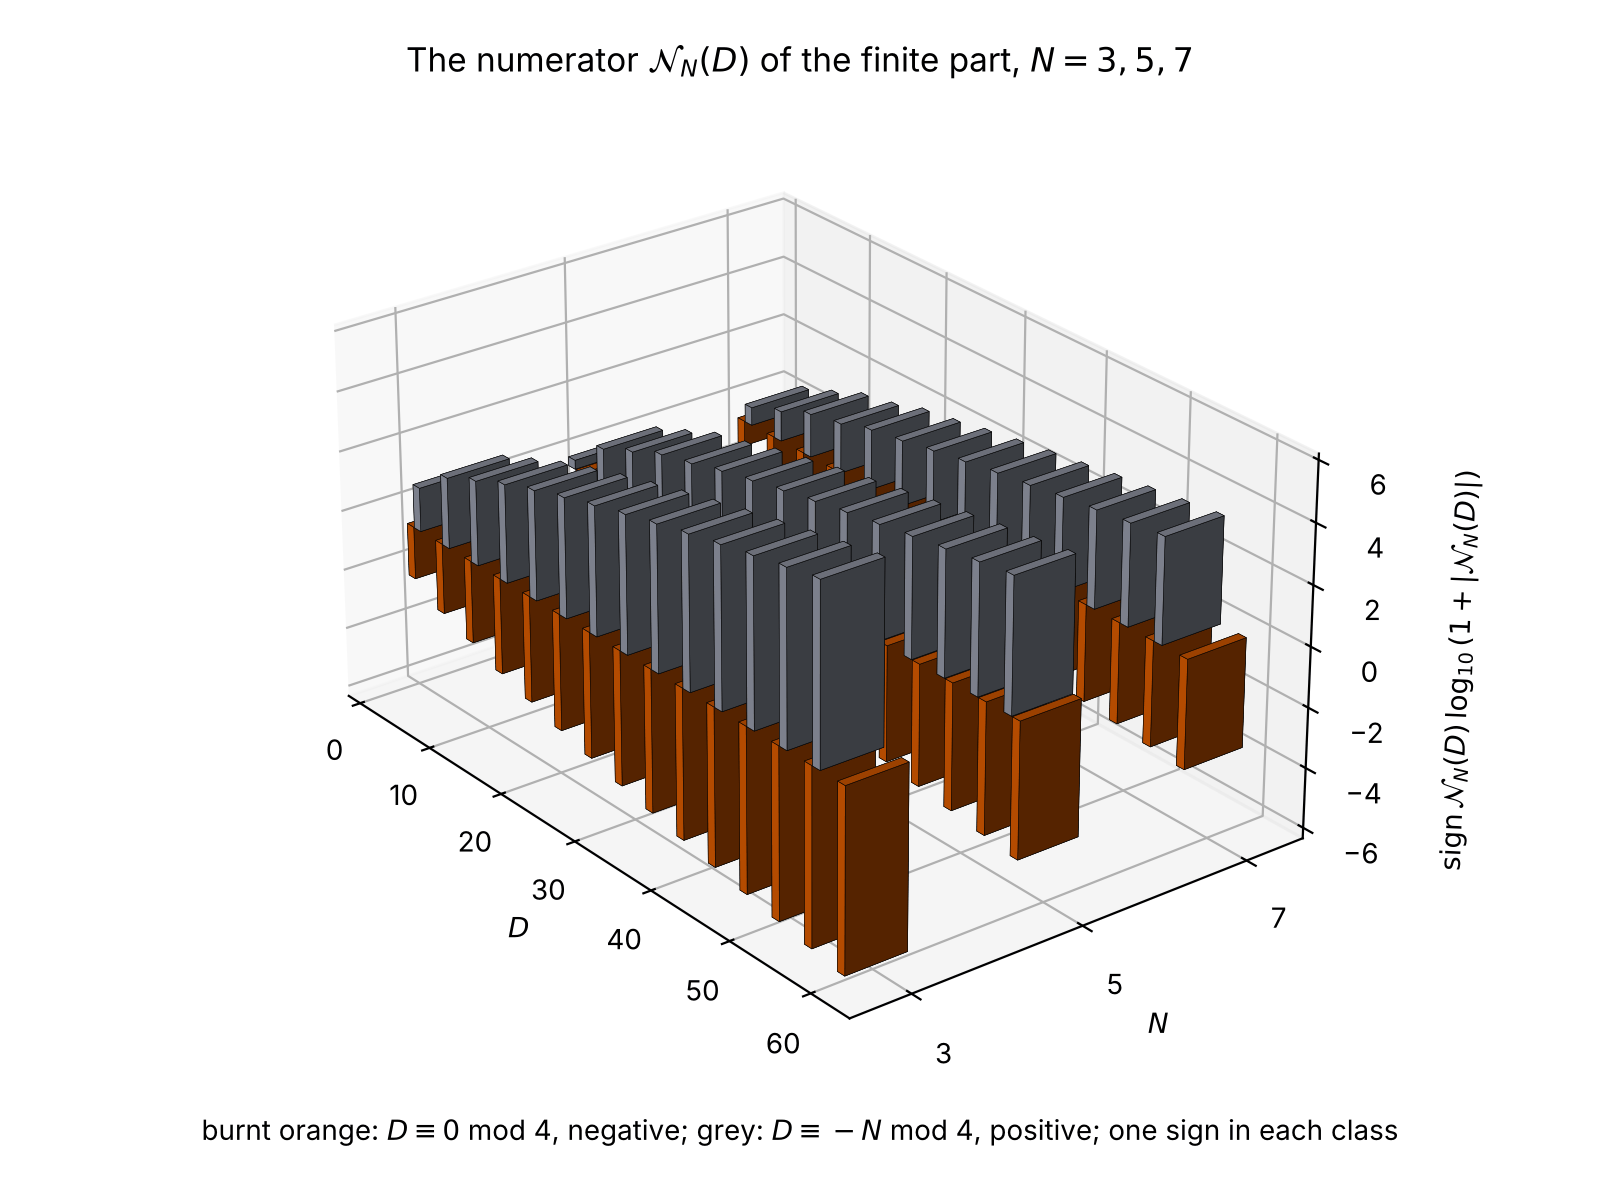
\includegraphics[width=0.94\linewidth,height=0.48\textheight,keepaspectratio]{figures/fig_chloddsigns.png}
\caption{The numerator $\mathcal N_N(D)$ of \eqref{eq:chlunioddcoeff} for $N=3,5,7$ and $D\le60$, on the scale $\mathrm{sign}\,\mathcal N\,\log_{10}(1+|\mathcal N|)$. It vanishes for $D\le0$ and off the two classes $D\equiv0$, $D\equiv-N\pmod4$; it is negative on the first and positive on the second (Lemma~\ref{lem:chlunioddsigns}).}
\label{fig:chloddsigns}
\end{figure}

\begin{theorem}\label{thm:chlunitodd}
In the $\ZZ_N$ CHL models with $N=3,5,7$ the single-centred index $d^*(Q,P)$ is positive for every charge with $NQ^2/2=1$, $P^2>0$ and $Q^2P^2>(Q\cdot P)^2$, and for every charge in the $\Gamma_1(N)$ orbit of such a charge.
\end{theorem}

\begin{proof}
The proof of Lemma~\ref{lem:chlunitsetA} holds for every $N$: at $m=1$ the quantity minimised in \cite[(5.47)]{BSS25} is $(m_1\ell+2s+1)^2+m_1^2\Delta/N$ with $m_1\in N\ZZ$, at least one. So $d^*=(-1)^{\ell+1}\mathcal C_N(\Delta)$ by Proposition~\ref{prop:chluniodd}, with $\Delta=4n-N\ell^2>0$ and $\Delta\equiv-N\ell^2\pmod 4$. Every argument $\Delta+4-4j$ of $\mathcal N_N$ in \eqref{eq:chlunioddcoeff} lies in the class of $\Delta$ modulo four, and every $\beta(j)$ is positive.\footnote{The sign of $d^*$ is thus decided by the term $j=0$ alone; the other terms have the same sign and only increase $|d^*|$. Figure~\ref{fig:chloddsigns} shows the two sign classes of $\mathcal N_N$.} If $\ell$ is odd, then $\Delta\ge1$, every term is $\ge0$ by Lemma~\ref{lem:chlunioddsigns}, and the term $j=0$ is $\mathcal N_N(\Delta+4)>0$. If $\ell$ is even, then $\Delta\ge4$, every term is $\le0$, and the term $j=0$ is $\mathcal N_N(\Delta+4)<0$. In both cases $d^*>0$. The orbits follow from the $\Gamma_1(N)$ invariance of $d^*$ \cite[(5.17)--(5.18)]{BSS25}.
\end{proof}

The first values, with $\Delta=N\big(Q^2P^2-(Q\cdot P)^2\big)$, are drawn in Figure~\ref{fig:chlodd}:\footnote{The least value is $d^*=3$, at $N=7$ and $\Delta=1$, the charge with $P^2=2$ and $Q\cdot P=1$. There $\mathcal N_7(1)=0$, so $d^*=\mathcal N_7(5)=\mu_7(3)-12c_7\,r_7(5)=9-6$, with $\mu_7(3)=\tfrac3{10}\big(28-c_7(3)\big)$, $c_7(3)=-2$ and $r_7(5)=4$.}
\[
\begin{array}{c|cccccccc}
N=3,\ \Delta&1&4&5&8&9&12&13&16\\
d^*&27&540&378&3294&2646&16200&14094&68418\\\hline
N=5,\ \Delta&3&4&7&8&11&12&15&16\\
d^*&20&100&125&460&588&1720&2191&5544\\\hline
N=7,\ \Delta&1&4&5&8&9&12&13&16\\
d^*&3&36&18&138&81&444&273&1242
\end{array}
\]

\begin{figure}[tbp]
\centering
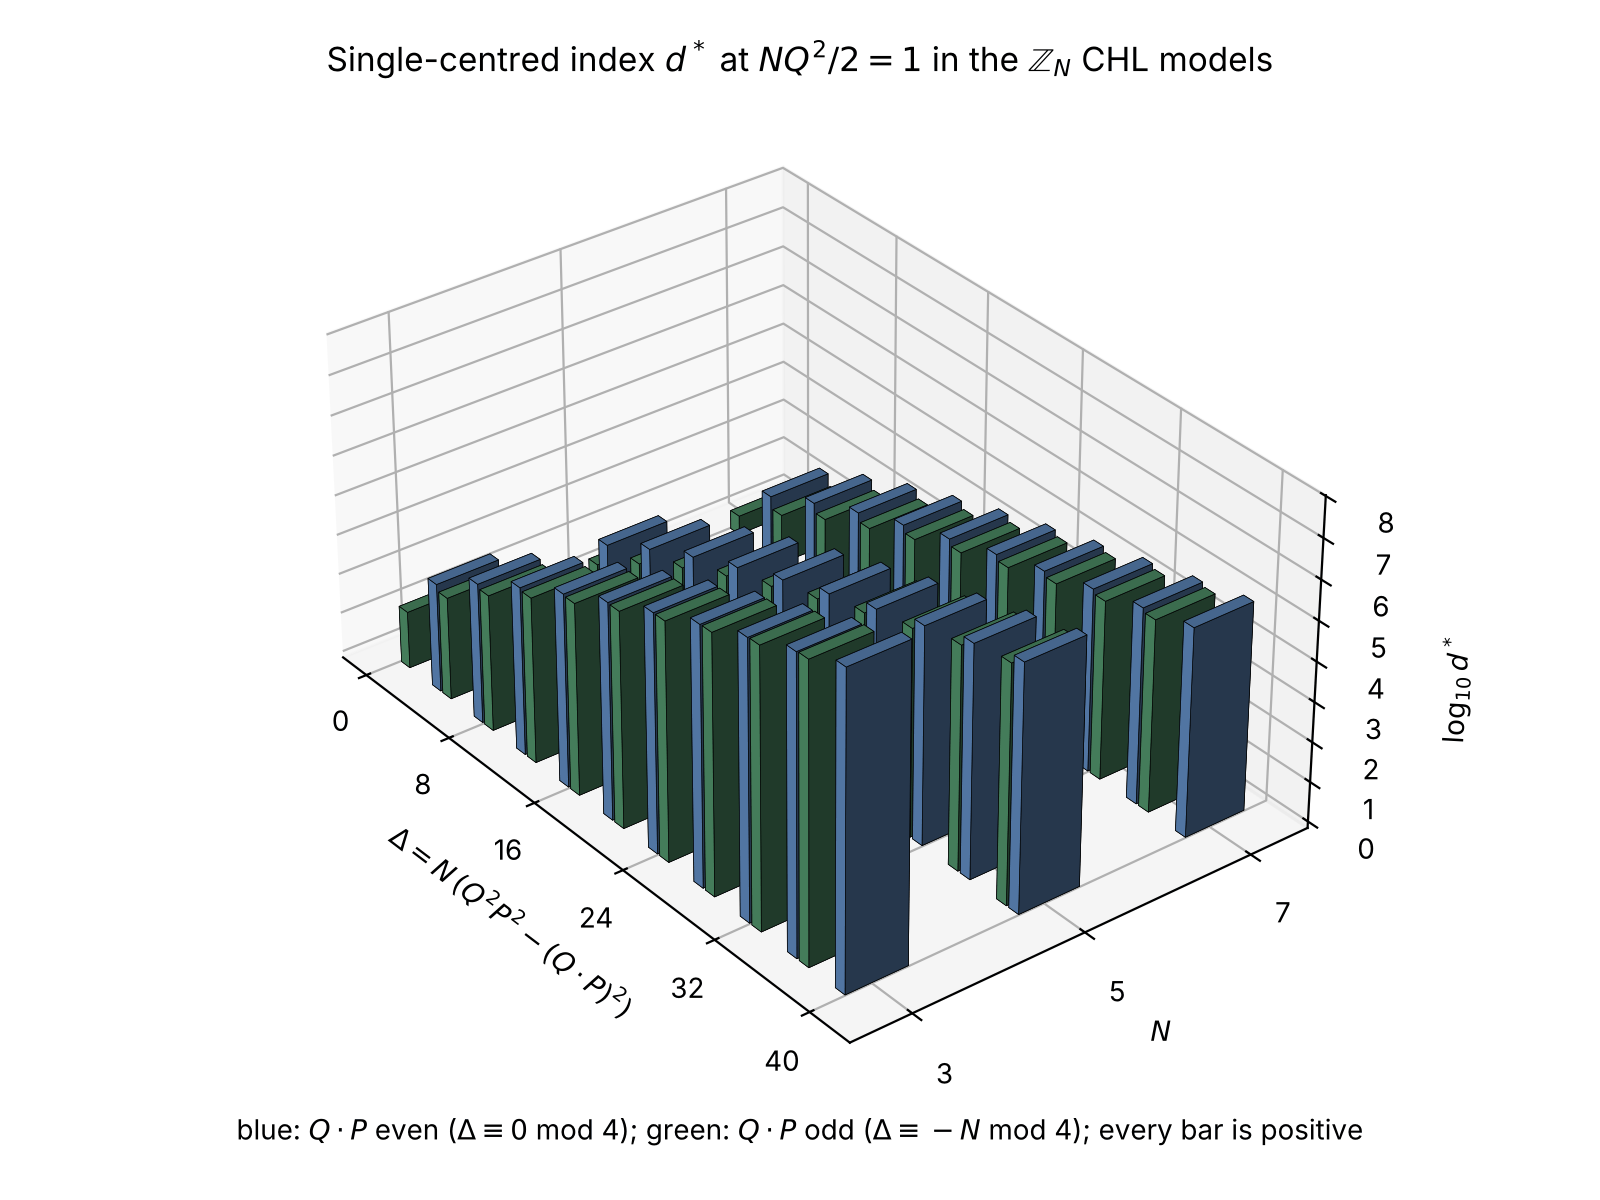
\includegraphics[width=0.94\linewidth,height=0.48\textheight,keepaspectratio]{figures/fig_chlodd.png}
\caption{The single-centred index $d^*$ at $NQ^2/2=1$ in the $\ZZ_N$ CHL models, $N=3,5,7$, for $\Delta\le40$, on the scale $\log_{10}d^*$. Blue bars have $Q\cdot P$ even, green bars $Q\cdot P$ odd; Theorem~\ref{thm:chlunitodd} proves positivity for every $\Delta$.}
\label{fig:chlodd}
\end{figure}

\subsection{Every charge of bounded discriminant}\label{ssec:chlbounded}

The two previous subsections settle the first electric charge. For the remaining charges we reduce the conjecture, discriminant by discriminant, to finitely many Fourier coefficients, and compute them. Let $N\in\{1,2,3,5,7\}$. For a charge write $m=NQ^2/2$, $n=P^2/2$, $\ell=Q\cdot P$, all integers, and
\[
\Delta=4mn-N\ell^2=N\big(Q^2P^2-(Q\cdot P)^2\big);
\]
for $N$ odd this is the $\Delta$ of Subsection~\ref{ssec:chlunitodd}, and for $N=2$ it is twice the $\Delta$ of Subsection~\ref{ssec:chlunit}. The charge form
\[
f_{Q,P}(s,t)=\tfrac N2\,(sQ+tP)^2=ms^2+N\ell\,st+Nn\,t^2
\]
has discriminant $-N\Delta$, and is positive definite when $m>0$ and $\Delta>0$; we assume this from now on. For a $2\times2$ matrix $g$ put $(f\circ g)(s,t)=f\big((s,t)g\big)$, so that $(f\circ g)\circ h=f\circ(hg)$. The group $\Gamma_1(N)$ of matrices $\gamma=\begin{psmallmatrix}a&b\\c&d\end{psmallmatrix}\in SL_2(\ZZ)$ with $c\equiv0$, $a\equiv d\equiv1\pmod N$ acts by $(Q,P)\mapsto(aQ+bP,cQ+dP)$, and $f_{\gamma(Q,P)}=f_{Q,P}\circ\gamma$.\footnote{This is the action of \cite[(5.17)--(5.19)]{BSS25} after the relabelling $\begin{psmallmatrix}a&b\\c&d\end{psmallmatrix}\mapsto\begin{psmallmatrix}d&c/N\\bN&a\end{psmallmatrix}$, and for $N=2$ the action of \cite[(3.8)]{Sen11positivity}.} The single-centred index $d^*$ is constant on the orbits \cite[Section~5.3]{BSS25}. A positive definite form $F=(A,B,C)=As^2+Bst+Ct^2$ is reduced if $|B|\le A\le C$, with $B\ge0$ when $|B|=A$ or $A=C$. Every positive definite form is $F\circ g$ for exactly one reduced $F$ and some $g\in SL_2(\ZZ)$ \cite[Theorem~2.8]{Cox13}, applied to the form divided by the greatest common divisor of its coefficients. A reduced form satisfies $3A^2\le4AC-B^2$, and, from the proof of that theorem,
\begin{equation}\label{eq:chlreduced}
F(x,y)\ge(A-|B|+C)\min(x^2,y^2),\qquad F(x,y)\ge C\ \text{ when } y\ne0 .
\end{equation}
Let $c(m,n,\ell)$ be the coefficient of $x^ny^\ell e^{2\pi im\rho}$ of $1/\Phit$ in the chamber $\operatorname{Im}v<0$ of Appendix~\ref{app:computation}, that is, the coefficient of $x^ny^\ell$ in $\varphi_m$ in the region $-\operatorname{Im}\sigma<\operatorname{Im}v<0$.

\begin{lemma}\label{lem:chlboundedcoef}
If $(Q,P)$ lies in the set $\mathcal A$ of \cite[(5.46)--(5.47)]{BSS25} and $0\le\ell\le 2m$, then $d^*(Q,P)=(-1)^{\ell+1}c(m,n,\ell)$.
\end{lemma}

\begin{proof}
By \cite[Theorem~5.4(a)]{BSS25}, $d^*=(-1)^{\ell+1}$ times the coefficient of $x^ny^\ell$ in the finite part $\varphi^F_m$, which has no poles and therefore one Fourier expansion. The polar part is \cite[(5.45)]{BSS25} a multiple of $g(\sigma/N)^{-1}\sum_{s\in\ZZ}p^{ms^2+s}y^{2ms+1}(1-p^sy)^{-2}$. In the region, $|p^sy|<1$ for $s\ge1$ and $|p^sy|>1$ for $s\le0$, so the term $s\ge1$ is a series in $y^{2ms+1+k}$, the term $s\le-1$ a series in $y^{2ms-1-k}$, and the term $s=0$ a series in $y^{-1-k}$, $k\ge0$. No exponent lies in $[0,2m]$, so at $y^\ell$ the coefficients of $\varphi_m$ and $\varphi^F_m$ agree.
\end{proof}

\begin{lemma}\label{lem:chlsetA}
Let $f=f_{Q,P}$. Then $(Q,P)\in\mathcal A$ if and only if $f(j,2k)\ge f(1,0)=m$ for every odd $j$ and every integer $k\ne0$ with $Nk\mid(j^2-1)/4$. A pair $(j,k)$ can violate this only if $|k|<m/\sqrt{N\Delta}$ and $|j+N\ell k/m|<1$, and the pairs $j=\pm1$ give exactly the condition $|\ell|\le2n$.
\end{lemma}

\begin{proof}
Condition (5.46) of \cite{BSS25} is $\Delta>0$. Condition (5.47) asks that $\big(N(m_1\ell+jm)^2+m_1^2\Delta\big)/(Nm^2)\ge1$ for every $m_1\in N\ZZ\setminus\{0\}$ and every $j=2s+1$ with $m_1\mid s(s+1)=(j^2-1)/4$; at $m=1$ this is the quantity of Lemma~\ref{lem:chlunitsetA}. With $m_1=Nk$,
\[
N(jm+N\ell k)^2+N^2k^2\Delta=Nm\big(mj^2+2N\ell jk+4Nnk^2\big)=Nm\,f(j,2k),
\]
which gives the criterion. Both terms on the left are nonnegative, so a violation needs $N^2k^2\Delta<Nm^2$ and $(jm+N\ell k)^2<m^2$. For $j=\pm1$ the condition is $k(\ell\pm2nk)\ge0$ for all $k\ne0$, which at $k=\pm1$ is $|\ell|\le 2n$ and for $|k|\ge2$ follows from it.
\end{proof}

\begin{theorem}\label{thm:chlleast}
Let $N\in\{1,2,3,5,7\}$. In every $\Gamma_1(N)$ orbit of charges, every charge whose $m=NQ^2/2$ is least in the orbit lies in $\mathcal A$, and the orbit contains such a charge with $0\le\ell<2m$. Hence $d^*$ of every charge with $Q^2>0$ and $Q^2P^2>(Q\cdot P)^2$ is $(-1)^{\ell+1}c(m,n,\ell)$ for a charge $(m,n,\ell)$ of least $m$ in its orbit.
\end{theorem}

\begin{proof}
Let $(Q,P)$ have least $m$, and let $(j,k)$ be as in Lemma~\ref{lem:chlsetA}. Every prime factor of $kN$ divides $(j^2-1)/4$, hence not $j$, and $j$ is odd; so $\gcd(j,2kN)=1$ and there are integers $c'$, $d$ with $jd-2kNc'=1$. Since $N$ divides $(j^2-1)/4$ and is $1$ or a prime, $j\equiv\varepsilon\pmod N$ with $\varepsilon=\pm1$.\footnote{This is the only place where $N$ is $1$ or a prime is used. The congruence $j\equiv\pm1\pmod N$ also follows from $4N\mid j^2-1$ for $N=4,6,8$, but not for $N=12$, where $j=7$.} Then
\[
\gamma=\varepsilon\begin{pmatrix}j&2k\\Nc'&d\end{pmatrix}
\]
has determinant one, lower left entry divisible by $N$, upper left entry $\varepsilon j\equiv1$, and lower right entry $\varepsilon d\equiv1\pmod N$ because $\varepsilon j\cdot\varepsilon d\equiv1$; so $\gamma\in\Gamma_1(N)$. The first coefficient of $f\circ\gamma$ is $f(\varepsilon j,2\varepsilon k)=f(j,2k)$, the $m$ of the charge $\gamma(Q,P)$, which is at least $m$ by minimality. Lemma~\ref{lem:chlsetA} gives $(Q,P)\in\mathcal A$. The matrix $\begin{psmallmatrix}1&0\\N\lambda&1\end{psmallmatrix}\in\Gamma_1(N)$ maps $(m,n,\ell)$ to $(m,\,n+N\lambda\ell+Nm\lambda^2,\,\ell+2m\lambda)$, the transformation \cite[(5.62)]{BSS25}; it keeps $m$ and moves $\ell$ into $[0,2m)$. The last statement is Lemma~\ref{lem:chlboundedcoef}.
\end{proof}

So the conjecture for the $\ZZ_N$ CHL model is the positivity of $(-1)^{\ell+1}c(m,n,\ell)$ at the charges of least $m$ in their orbits, and these charges are found by reduction theory.

\begin{lemma}\label{lem:chlorbits}
Let $N$ be $1$ or a prime, and $f_{Q,P}=F\circ g$ with $F$ reduced and $g\in SL_2(\ZZ)$ of lower row $(c,d)$.

\textup{(i)} The orbit of $(Q,P)$ consists of the charges whose forms are $F\circ g'$, where $g'\in SL_2(\ZZ)$ has lower row congruent modulo $N$ to $(c,d)h$ for some $h$ in the group $\operatorname{Aut}(F)$ of $h\in SL_2(\ZZ)$ with $F\circ h=F$.

\textup{(ii)} For a reduced form $F$ of discriminant $-N\Delta$ and a row $(c,d)$, primitive modulo $N$, with $F(c,d)\equiv0\pmod N$, every $F\circ g'$ with lower row $(c,d)$ is a charge form exactly when its middle coefficient is divisible by $N$, and this does not depend on the upper row of $g'$.

So the orbits of discriminant $\Delta$ correspond to the pairs of a reduced form of discriminant $-N\Delta$ and an admissible row modulo $N$, up to $\operatorname{Aut}(F)$, and there are finitely many.
\end{lemma}

\begin{proof}
(i) By $(f\circ g)\circ h=f\circ(hg)$, the forms of the orbit are $F\circ(\gamma g)$, $\gamma\in\Gamma_1(N)$, and $F\circ g'=F\circ g$ exactly when $g'\in g\operatorname{Aut}(F)$. The lower row of $\gamma g$ is $(0,1)\gamma g\equiv(c,d)$, and if $g$, $g'$ have congruent lower rows then $g'g^{-1}$ has lower row congruent to $(0,1)$ and lies in $\Gamma_1(N)$. So the orbit is the set of $F\circ g'$ with $g'\in\Gamma_1(N)\,g\operatorname{Aut}(F)$, whose lower rows are the rows congruent to $(c,d)h$.
(ii) The last coefficient of $F\circ g'$ is $F(c,d)$. The upper rows with lower row $(c,d)$ differ by multiples of $(c,d)$, and adding $k(c,d)$ changes the middle coefficient by $2kF(c,d)$.
\end{proof}

\begin{proposition}\label{prop:chlsize}
\textup{(i)} For $N\in\{2,3\}$ every orbit contains a charge of $\mathcal A$ with $0\le\ell<2m$ and $\min(m,n)\le\sqrt{N\Delta/3}$.

\textup{(ii)} For $N\in\{5,7\}$, $h=(N+1)/2$ and every $j\ge1$, every charge in the orbit of
\[
(m,n,\ell)=\big(h^2+Nj,\ N+4j,\ N+1+4j\big),\qquad \Delta=4j,
\]
has $m\ge N\Delta/4$ and $n\ge\Delta$.
\end{proposition}

\begin{proof}
(i) Let $f_{Q,P}=F\circ g$ as in Lemma~\ref{lem:chlorbits}, $F=(A,B,C)$, so that $A\le\sqrt{N\Delta/3}$. Every nonzero residue modulo $N=2,3$ is $\pm1$. If some row $(c,d)h$, $h\in\operatorname{Aut}(F)$, has second entry not divisible by $N$, call it $(c,d)$ again and take $g'=\begin{psmallmatrix}e&0\\c&e\end{psmallmatrix}$ with $e=\pm1\equiv d$: the charge $F\circ g'$ of the orbit has $m=F(e,0)=A$, the least value of $F$, and Theorem~\ref{thm:chlleast} applies. Otherwise every lower row in the class has $d\equiv0$, so every upper row $(x,y)$ in the orbit has $y\ne0$ (for $y=0$ the determinant forces $d=\pm1$), and every charge has $m\ge C$ by \eqref{eq:chlreduced}. The row $(e,0)$, $e=\pm1\equiv c$, is admissible. If $B\le0$, the matrix $\begin{psmallmatrix}0&-e\\e&0\end{psmallmatrix}$ gives $(m,n,\ell)=(C,A/N,-B/N)$, of least $m$ and with $0\le\ell<2m$. If $B>0$, the matrix $\begin{psmallmatrix}e&-e\\e&0\end{psmallmatrix}$ gives $f(s,t)=F(s+t,-s)$ and $(m,n,\ell)=(A-B+C,\,A/N,\,(2A-B)/N)$, with $0\le\ell<2m$ since $B\le A\le C$. Here $f(j,2k)=F(j+2k,-j)$ with both arguments odd, so $f(j,2k)\ge A-|B|+C=m$ by \eqref{eq:chlreduced}, and the charge lies in $\mathcal A$ by Lemma~\ref{lem:chlsetA}. In each case $\min(m,n)\le A$.

(ii) With $F=(1,0,Nj)$ and $g=\begin{psmallmatrix}h&1\\N&2\end{psmallmatrix}$, $F\circ g=(h^2+Nj,\,N(N+1+4j),\,N(N+4j))$ is the form of the charge, of discriminant $-4Nj$. Here $\operatorname{Aut}(F)=\{\pm1\}$, so every $g'$ of the orbit has lower row $(c',d')\equiv\pm(0,2)$, and its upper row $(x,y)$ satisfies $2x\equiv\pm1$, that is $x\equiv\pm h\pmod N$. Since $h\not\equiv\pm1\pmod N$ for $N=5,7$, $y\ne0$, and $m=x^2+Njy^2\ge Nj$. Since $d'\equiv\pm2$, $|d'|\ge2$, and $n=(c'^2+Njd'^2)/N\ge4j$.
\end{proof}

So for $N=2,3$ the least $m$ or the least $n$ of an orbit is at most $\sqrt{N\Delta/3}$, while for $N=5,7$ both grow linearly with $\Delta$ along infinitely many orbits.\footnote{For $N=3$ the charge of (ii) is $(4+3j,3+4j,4+4j)$, but $h=2\equiv-1\pmod 3$ and the orbit contains $(1,j,0)$.} The orbits of (ii) are the reason for the different ranges of the next theorem.

\begin{theorem}\label{thm:chlbounded}
In the $\ZZ_N$ CHL models with $N=2,3,5,7$ the single-centred index $d^*(Q,P)$ is positive for every charge with $Q^2>0$ and
\[
0<Q^2P^2-(Q\cdot P)^2\le\frac{\Delta_N}N,\qquad \Delta_2=\Delta_3=1000,\quad\Delta_5=100,\quad \Delta_7=60,
\]
that is $Q^2P^2-(Q\cdot P)^2\le500$, $1000/3$, $20$, $60/7$. These charges form $11\,237$, $12\,276$, $876$ and $668$ orbits of $\Gamma_1(N)$, and the least values of $d^*$ are $360$, $27$, $20$ and $3$, at the charges $(m,n,\ell)=(1,1,1)$, $(1,1,1)$, $(1,2,1)$ and $(1,2,1)$ of Theorems~\ref{thm:chlunit} and~\ref{thm:chlunitodd}.
\end{theorem}

\begin{proof}
For each $\Delta\le\Delta_N$, Lemma~\ref{lem:chlorbits} lists the orbits. In each orbit we find a charge of $\mathcal A$ with $0\le\ell<2m$: it exists by Theorem~\ref{thm:chlleast}, it is tested by Lemma~\ref{lem:chlsetA}, and for $N=2,3$ Proposition~\ref{prop:chlsize}(i) bounds the search by $\min(m,n)\le\sqrt{N\Delta/3}$. By Lemma~\ref{lem:chlboundedcoef}, $d^*=(-1)^{\ell+1}c(m,n,\ell)$, and $c(m,n,\ell)$ is computed from the product formula \eqref{eq:product} as in Appendix~\ref{app:computation}, in exact integer arithmetic.\footnote{The exponents of \eqref{eq:product} are symmetric under the exchange of their first two indices on the whole range used, and the chamber $\operatorname{Im}v<0$ is the domain of absolute convergence of the product, which is symmetric under $\rho\leftrightarrow\sigma$; so $c(m,n,\ell)=c(n,m,\ell)$ there, and each coefficient is read in the orientation with the smaller first index.} Every value is positive. The program \cite{Bha26} also checks that every second charge of $\mathcal A$ found in an orbit gives the same value, that the values at $m=1$ are those of Theorems~\ref{thm:chlunit} and~\ref{thm:chlunitodd}, and Theorem~\ref{thm:chlleast} itself on the whole range.
\end{proof}

The theorem contains Theorems~\ref{thm:chlpositivity}, \ref{thm:chlunit} and~\ref{thm:chlunitodd} in its range; outside it, these three hold for every $\Delta$.

\begin{remark}\label{rem:chlbssB}
Bhand, Sen and Singh also define a set $\mathcal B$ \cite[(5.48)--(5.49)]{BSS25}, like $\mathcal A$ with the roles of $Q$ and $P$ exchanged, on which $d^*$ is a Fourier coefficient of the finite part $\psi^F_n$ of the expansion in $e^{2\pi i\sigma}$, and they state that the set $B_2$ of charges with $Nm\ge n$ and $|\ell|\le2n$ lies in $\mathcal B$ \cite[(5.65) and (B.36)]{BSS25}. For $N\ge2$ this containment fails. For $N=2$ the charges $(m,n,\ell)=(1,1,1)$ and $(5,5,7)$, both with $\Delta=2$, lie in $B_2$ and in one orbit, the second being the image of the first under $\begin{psmallmatrix}-3&1\\-4&1\end{psmallmatrix}\in\Gamma_1(2)$; since $0\le\ell\le2n$, the polar part of $\psi_n$ does not contribute, as in Lemma~\ref{lem:chlboundedcoef}, and the coefficients $(-1)^{\ell+1}c(m,n,\ell)$ are $360$ and $3064$. For $N=7$ the charges $(1,2,1)$ and $(29,44,27)$, with $\Delta=1$, related by $\begin{psmallmatrix}15&-4\\49&-13\end{psmallmatrix}\in\Gamma_1(7)$, give $3$ and $201$. The first charge of each pair lies in $\mathcal A$, so $d^*=360$ and $d^*=3$ on the two orbits, and neither second charge lies in $\mathcal B$. The step of the proof that fails is (B.37), where the quantity $(m_1+jN\ell/2n)/n_1$ is replaced by its quotient by $N^2$, which is smaller when it is positive. At $P^2=2$ the conditions defining $\mathcal B$ are empty, so Theorem~\ref{thm:chlpositivity} does not depend on this step; Theorems~\ref{thm:chlleast} and~\ref{thm:chlbounded} use only $\mathcal A$.
\end{remark}

\begin{figure}[tbp]
\centering
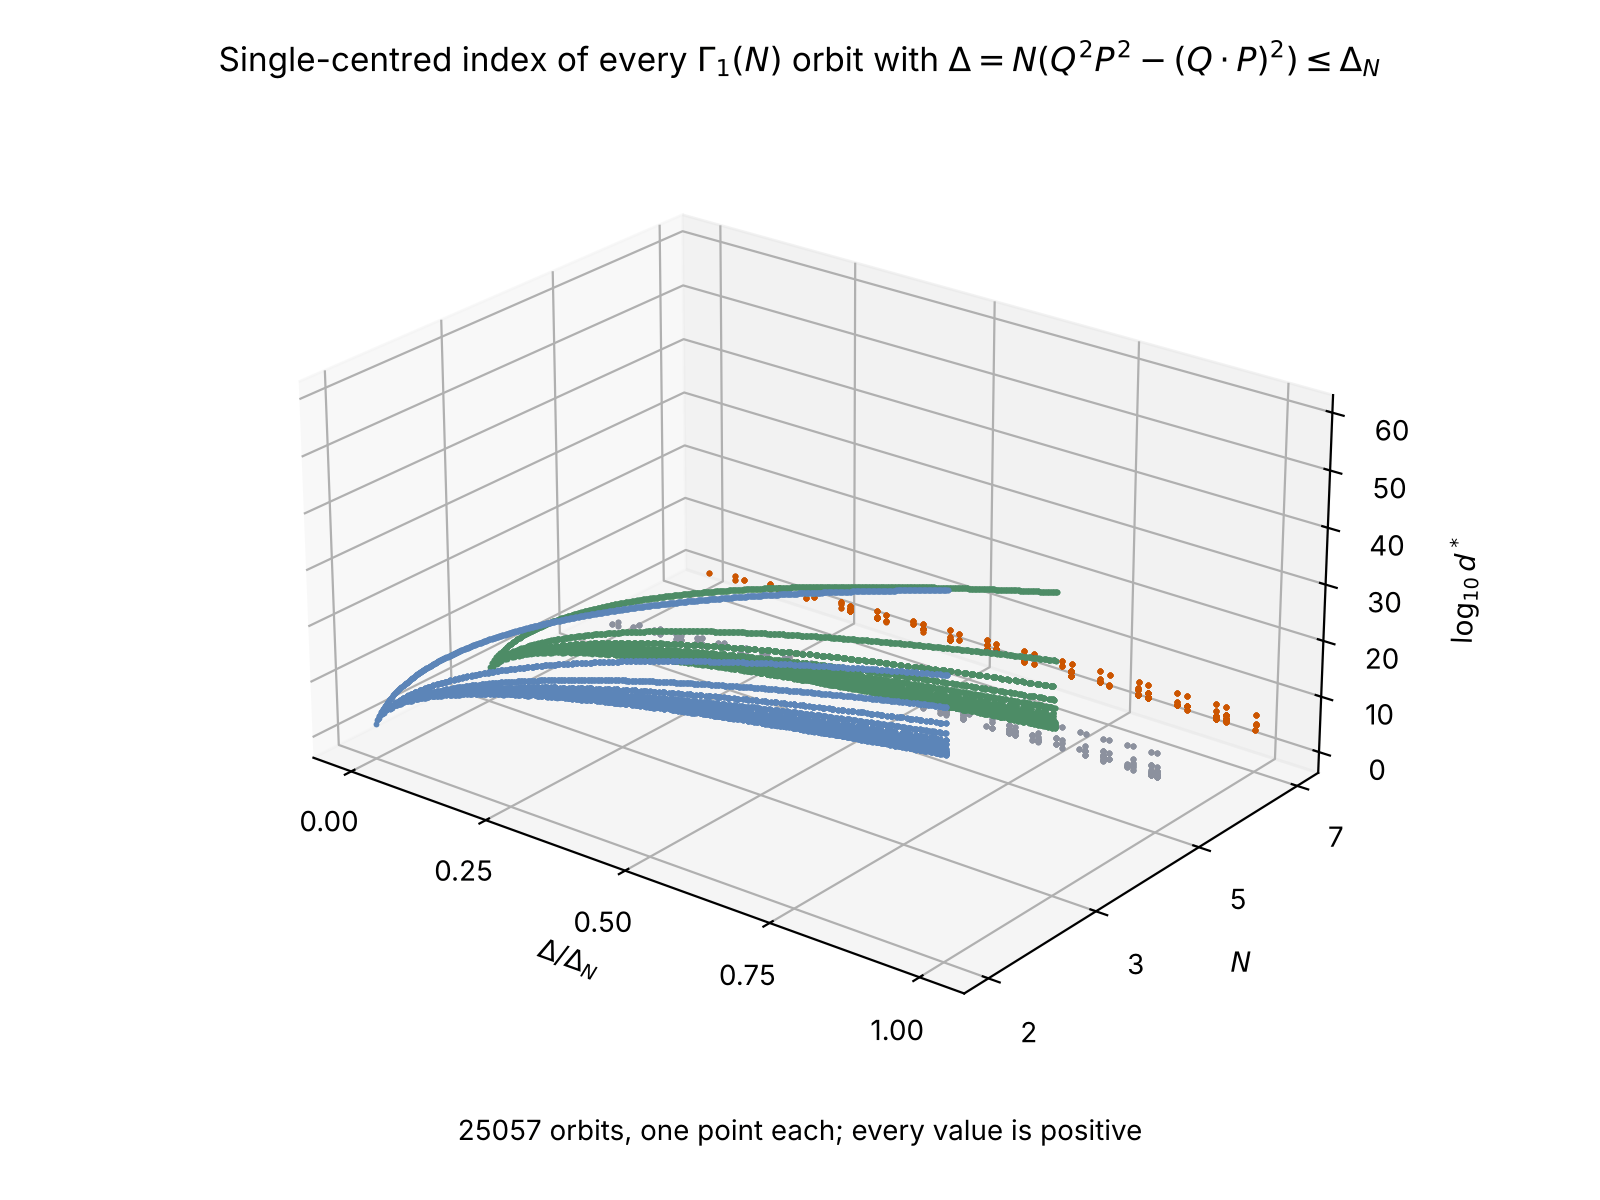
\includegraphics[width=0.94\linewidth,height=0.46\textheight,keepaspectratio]{figures/fig_chlbounded.png}
\caption{The single-centred index of every $\Gamma_1(N)$ orbit with $\Delta=N\big(Q^2P^2-(Q\cdot P)^2\big)\le\Delta_N$, on the scale $\log_{10}d^*$, for $N=2,3$ ($\Delta\le1000$), $N=5$ ($\Delta\le100$) and $N=7$ ($\Delta\le60$). Each point is one orbit; every value is positive (Theorem~\ref{thm:chlbounded}).}
\label{fig:chlbounded}
\end{figure}

\begin{figure}[tbp]
\centering
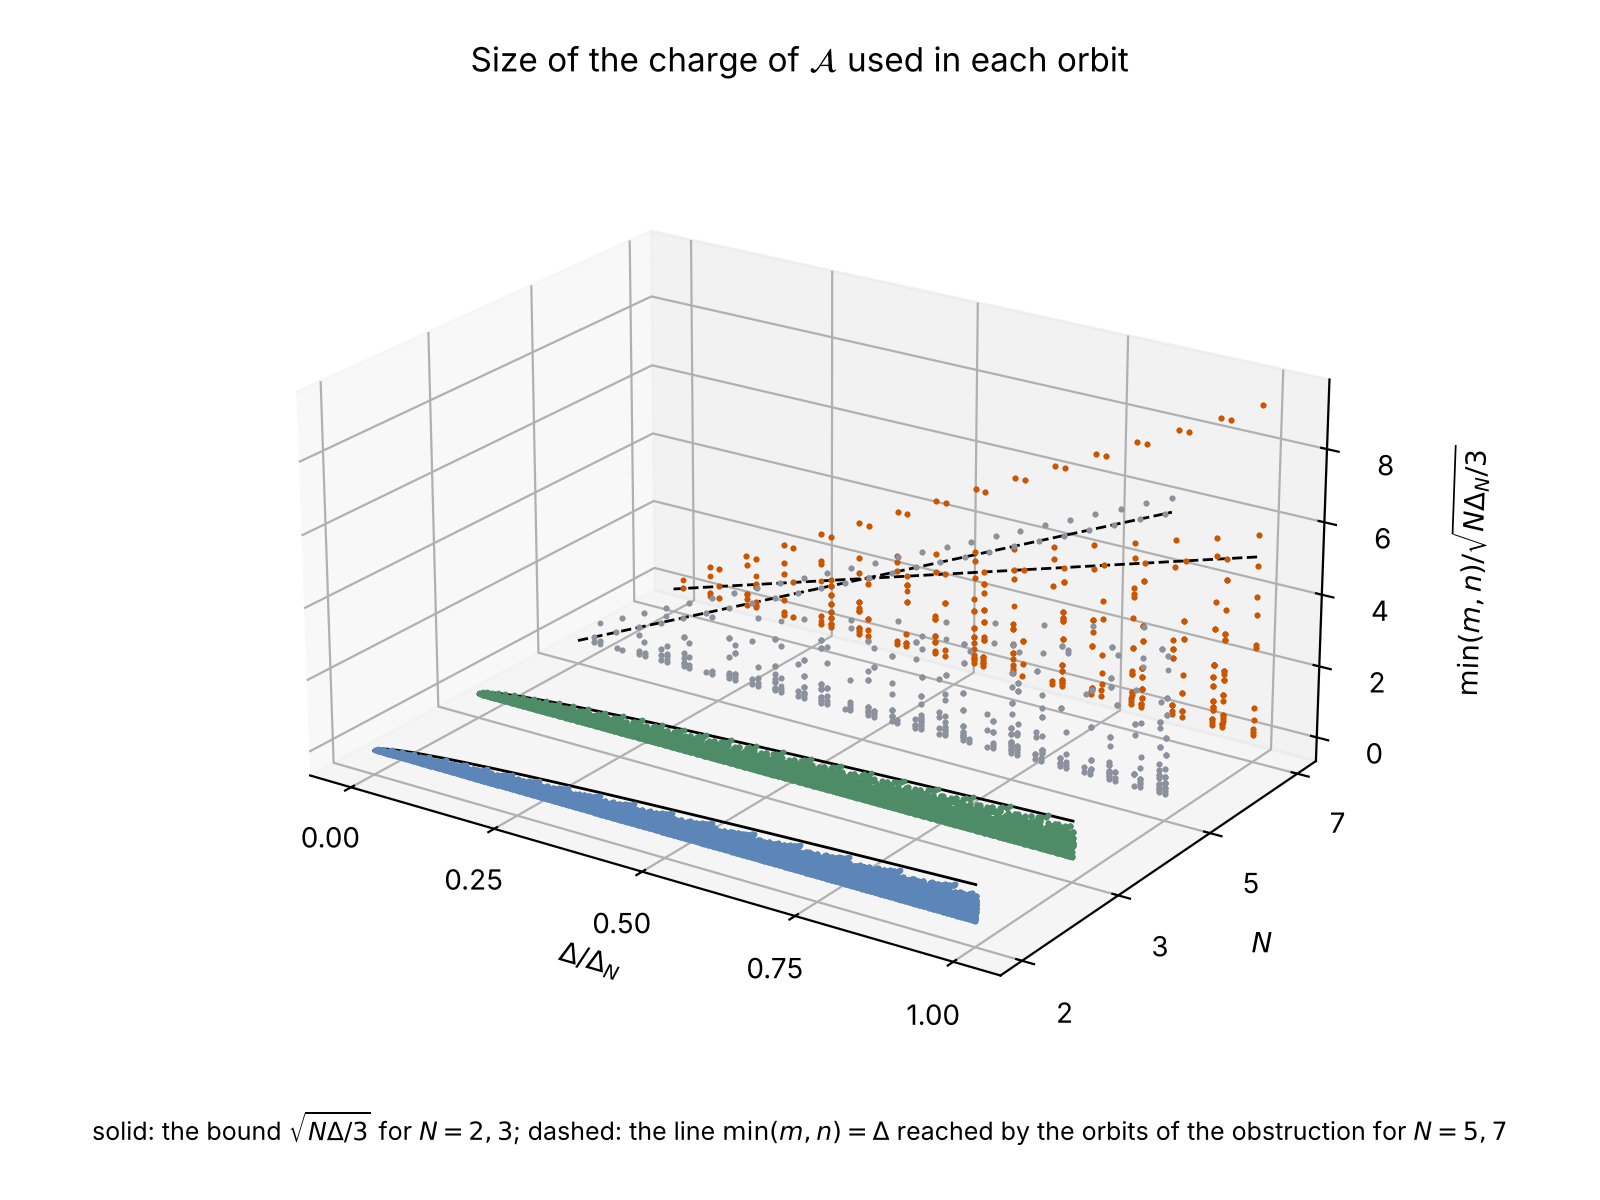
\includegraphics[width=0.94\linewidth,height=0.46\textheight,keepaspectratio]{figures/fig_chlsize.png}
\caption{The smaller of $m$ and $n$ at the charge of $\mathcal A$ used for each orbit, against $\Delta$. For $N=2,3$ it stays below $\sqrt{N\Delta/3}$ (Proposition~\ref{prop:chlsize}(i)); for $N=5,7$ the orbits of Proposition~\ref{prop:chlsize}(ii) force growth along the line $\Delta$.}
\label{fig:chlsize}
\end{figure}

\begin{remark}\label{rem:chlunitopen}
At $NQ^2/2=1$ the mock and holomorphic pieces of the finite part are class numbers and theta coefficients of a lattice of rank four, both dominated by a cubic divisor sum of fixed sign; this is the mechanism of Theorems~\ref{thm:chlunit} and~\ref{thm:chlunitodd}, and of Theorem~\ref{thm:chlpositivity} at $P^2=2$. Theorem~\ref{thm:chlleast} removes the reduction problem: every orbit meets $\mathcal A$ at its charges of least $NQ^2/2$, where $d^*$ is a Fourier coefficient of $\varphi^F_m$. What remains for every charge is the sign of these coefficients for every $m\ge2$, with $0\le\ell<2m$ and $n$ unbounded. For $m\ge2$ the finite parts contain mock pieces of higher index for $\Gamma^0(N)$ that are not class number generating functions, and a proof needs an explicit bound of their Rademacher tails at the cusps of $\Gamma_0(N)$ against the leading Bessel term, uniform in $m$. For $N=5,7$ a finite set of $m$ does not suffice, since by Proposition~\ref{prop:chlsize}(ii) the least $m$ grows linearly with $\Delta$ along infinitely many orbits.
\end{remark}

\begin{verdict}[claim 9, heterotic and CHL]
Proved for the heterotic string on $T^6$ at $P^2\in\{2,4\}$, with all $Q$ and $Q\cdot P$ satisfying $Q^2P^2>(Q\cdot P)^2$, and on the $SL(2,\ZZ)$ orbits of these charges (Theorem~\ref{thm:bringmannmurthy}). Proved for the $\ZZ_2$ CHL model at $P^2=2$ with every $Q$, at $NQ^2/2=1$ with every $P$, and on the $\Gamma_1(2)$ orbits of these charges (Theorems~\ref{thm:chlpositivity} and~\ref{thm:chlunit}). Proved for the $\ZZ_N$ CHL models with $N=3,5,7$ at $NQ^2/2=1$ with every $P$, and on the $\Gamma_1(N)$ orbits of these charges (Theorem~\ref{thm:chlunitodd}). For $N=2,3,5,7$ every orbit is reduced to one Fourier coefficient of $\varphi^F_m$ at its least $NQ^2/2=m$ (Theorem~\ref{thm:chlleast}), and positivity is proved, with computer assistance, for every charge with $N\big(Q^2P^2-(Q\cdot P)^2\big)\le1000$ when $N=2,3$, $\le100$ when $N=5$ and $\le60$ when $N=7$ (Theorem~\ref{thm:chlbounded}). Our scan of the heterotic cone up to $Q^2\le 12$, $P^2\le 6$, $Q\cdot P\le 4$ (Appendix~\ref{app:computation}) finds only positive indices. \gap{A proof of positivity for every charge is not known: for the heterotic string it is open at $P^2\ge6$ outside the $SL(2,\ZZ)$ orbits of the charges with $P^2\le4$, and for $N=2,3,5,7$ it is open on the orbits whose least $NQ^2/2$ is at least two (for $N=2$, whose least $P^2$ is also at least four) and whose $N\big(Q^2P^2-(Q\cdot P)^2\big)$ exceeds $1000$, $1000$, $100$, $60$.} Remark~\ref{rem:chlunitopen} lists what a proof of the remaining cases needs.
\end{verdict}

\subsection{Full and horizon indices in the toroidal orbifolds}\label{ssec:toroidal}

Sen's paper states the conjecture as a consequence of the black hole argument for ``the $\mathcal N=4$ supersymmetric string theories'', and the subsequent literature \cite{CD19,CKMRW20} tested it in the full list of $\mathcal N=4$ compactifications with known dyon partition functions. Chattopadhyaya and David \cite{CD19} found that it fails in two of them: the freely acting $\ZZ_2$ and $\ZZ_3$ orbifolds of type IIB on $T^6$, in which the orbifold acts by a reflection of four coordinates of $T^4$ (or a rotation by $2\pi/3$ of two planes) together with a shift of half (or a third) of a circle of the remaining $T^2$. The $\ZZ_2$ model has the twisted elliptic genera
\begin{equation}\label{eq:tor2genera}
\begin{aligned}
F^{(0,0)} &= 0,& F^{(0,1)} &= \tfrac83 A - \tfrac43 B\,E_2(\tau),\\
F^{(1,0)} &= \tfrac83 A + \tfrac23 B\,E_2(\tfrac\tau2),& F^{(1,1)} &= \tfrac83 A + \tfrac23 B\,E_2(\tfrac{\tau+1}2),
\end{aligned}
\end{equation}
where $A = \sum_{i=2}^4\theta_i(\tau,z)^2/\theta_i(\tau,0)^2$, $B = \theta_1(\tau,z)^2/\eta(\tau)^6$, and $E_2(\tau) := 2E(2\tau) - E(\tau)$ is the weight-two form of $\Gamma_0(2)$ built from the Eisenstein series $E(\tau) = 1 - 24\sum\sigma_1(n)q^n$ (the $E_N$ of \cite{DJS06}, not the quasi-modular Eisenstein series). The Siegel form is $\Phit_2 = \Phit_6^2/\Phit_{10}$, of weight two, with the prefactor $e^{2\pi i(\rho+v)}$ in place of $e^{2\pi i(\rho+\sigma/N+v)}$ in \eqref{eq:product}, and the index is given by \eqref{eq:dvv} with $Q^2\in\ZZ$, $P^2\in 2\ZZ$. The single-centred region is again cut out by \eqref{eq:z2conditions}, since the duality group is again $\Gamma_1(2)$.

\begin{theorem}[known negative full indices; finite exact test]\label{thm:positivityfails}
In the $\ZZ_2$ toroidal orbifold of type IIB on $T^6$, the index $d(Q,P)$ computed from \eqref{eq:dvv} with the contour of the attractor region is negative for infinitely many charges satisfying the single-centred conditions \eqref{eq:z2conditions}. In the range $Q^2\le 12$, $P^2\le 8$, $Q\cdot P\le 4$ there are exactly thirty such charge triples, listed in Table~\ref{tab:violations}; the first ones are
\begin{gather*}
d(1,2,0) = -224,\quad d(1,4,0) = -1248,\\
d(2,2,1) = -256,\quad d(3,2,0) = -3392,\\
d(3,4,0) = -10320,
\end{gather*}
in the notation $d(Q^2,P^2,Q\cdot P)$. In the first column of Table~\ref{tab:tor2} ($P^2=0$, outside the cone) the sign is $(-1)^{Q^2}$ for $Q^2\le 12$; Figure~\ref{fig:indices} draws the table.
\end{theorem}

\begin{figure}[tbp]
\centering
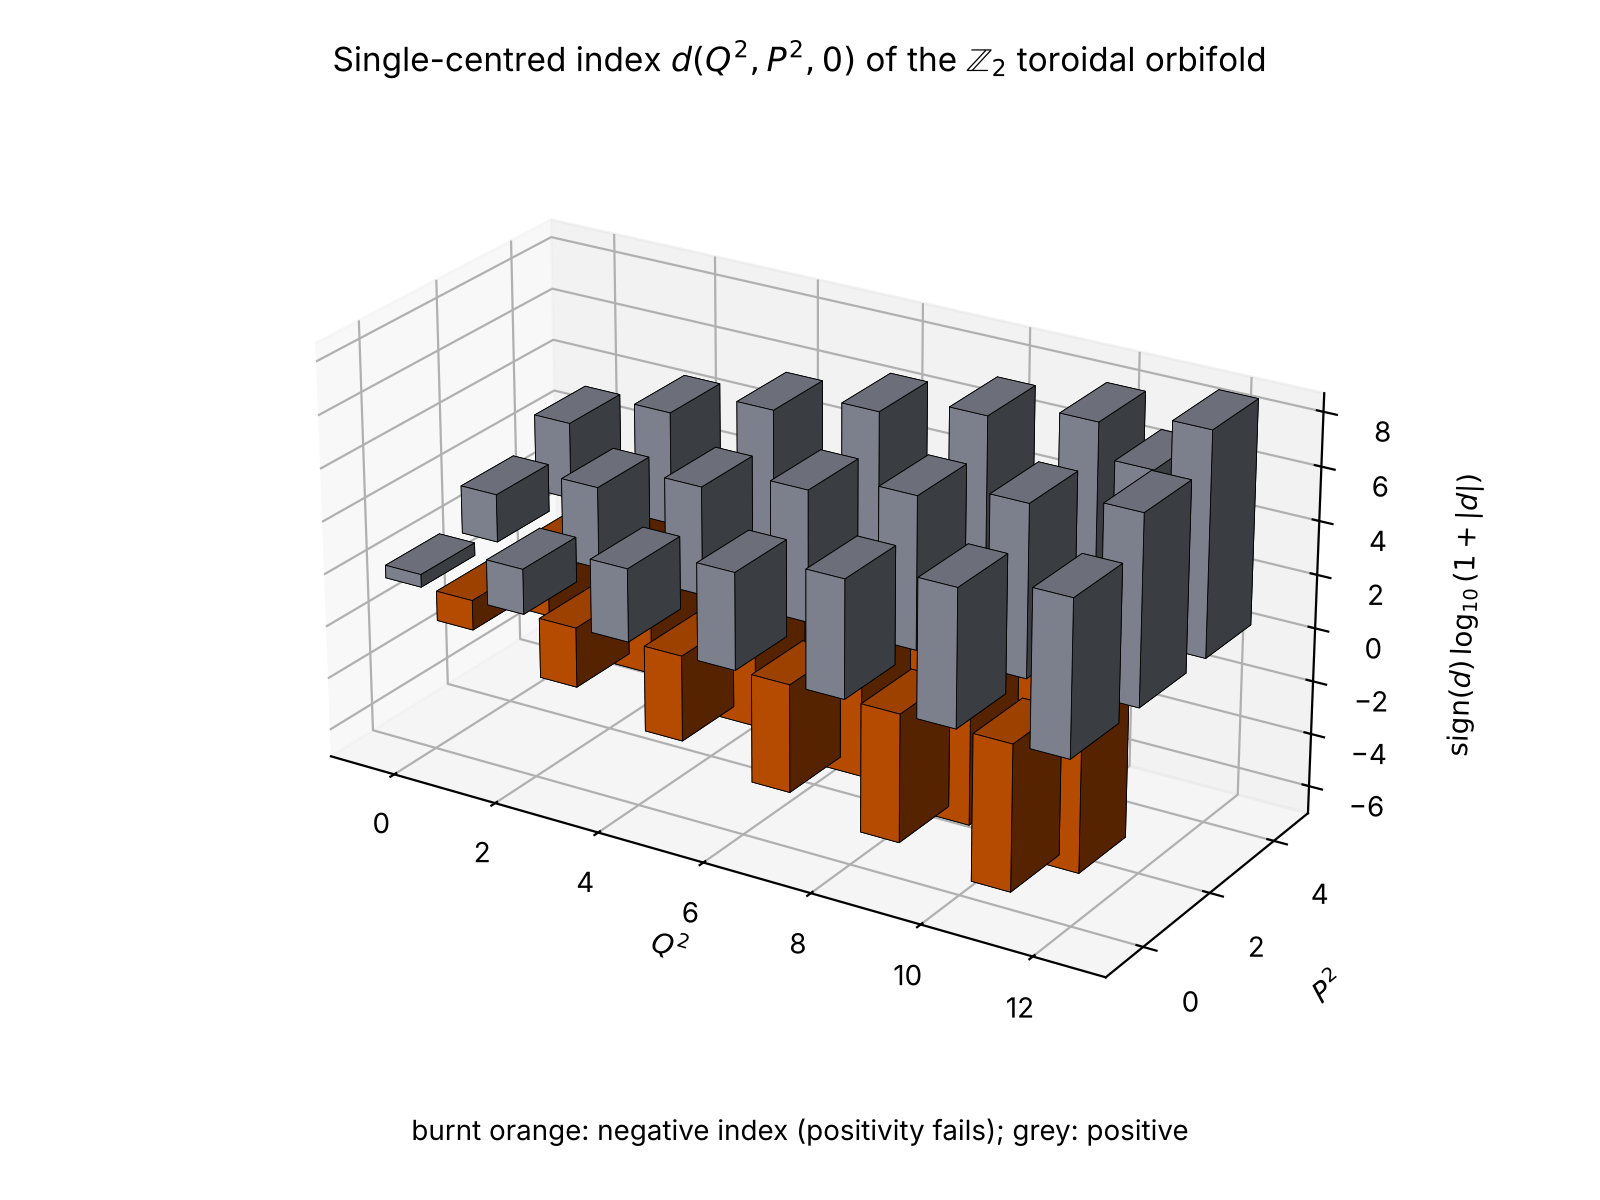
\includegraphics[width=0.94\linewidth,height=0.48\textheight,keepaspectratio]{figures/fig_indices.png}
\caption{The full index $d(Q^2,P^2,0)$ of the $\ZZ_2$ toroidal orbifold from Table~\ref{tab:tor2}, drawn on the scale $\mathrm{sign}(d)\log_{10}(1+|d|)$. Every bar in burnt orange is a negative full index; along $P^2 = 2$ the sign alternates with $Q^2$, and every odd $Q^2$ lies inside the cone \eqref{eq:z2conditions} of Theorem~\ref{thm:positivityfails}. A horizon index requires the separate hair analysis.}
\label{fig:indices}
\end{figure}

\begin{proof}
We expanded the product \eqref{eq:product} for the genera \eqref{eq:tor2genera} in exact rational arithmetic, with the Fourier coefficients of the theta functions, of $\eta^{-6}$ and of the Eisenstein series computed from their definitions, and read off the coefficients in the convention $q_\rho=e^{2\pi i\rho}$, $q_\sigma=e^{2\pi i\sigma/N}$ and $y=e^{2\pi iv}$, keyed by $(NQ^2/2,P^2/2,Q\cdot P)$ in the expansion in which the factor $(1-e^{-2\pi i v})^{-2}$ at $k'=l=0$ is expanded in powers of $e^{-2\pi iv}$ (the attractor region for $Q\cdot P\ge 0$). The resulting tables agree entry by entry with Tables~17, 18 and~19 of \cite{CD19} in their common range. The thirty charge triples of Table~\ref{tab:violations} satisfy each inequality of \eqref{eq:z2conditions} by inspection and have negative index. For the infinitude: the values at $P^2=2$, $Q\cdot P=0$ are
\[
\begin{gathered}
64,\ -224,\ 1152,\ -3392,\ 11520,\ -30336,\ 83968,\\
-202560,\ 496512,\ -1118496,\ 2521600,\ -5374656
\end{gathered}
\]
for $Q^2 = 0,1,2,\dots,11$; every odd $Q^2$ with $P^2 = 2$, $Q\cdot P = 0$ lies in the cone \eqref{eq:z2conditions}, and \cite[Section~4.1]{CD19} show from the Fourier--Jacobi coefficient $\psi_1$ of $1/\Phit_2$ at $P^2=2$ that the finite part of $\psi_1$, which is what the single-centred index is, has coefficients of alternating sign in $Q^2$; the alternation is visible in our table for $Q^2\le 12$. The analogous statement for the $\ZZ_3$ orbifold is \cite[Section~4.2]{CD19}.
\end{proof}

\begin{table}[tbp]
\centering\scriptsize
\begin{tabular}{@{}rrrr@{\quad}rrrr@{}}
\toprule
$Q^2$&$P^2$&$Q\cdot P$&$d$&$Q^2$&$P^2$&$Q\cdot P$&$d$\\
\midrule
1 & 2 & 0 & -224 & 6 & 2 & 1 & -33536 \\
1 & 4 & 0 & -1248 & 7 & 2 & 0 & -202560 \\
1 & 6 & 2 & -224 & 7 & 2 & 2 & -30336 \\
1 & 8 & 2 & -1248 & 7 & 4 & 0 & -179022 \\
2 & 2 & 1 & -256 & 7 & 4 & 4 & -10320 \\
2 & 6 & 3 & -256 & 8 & 2 & 1 & -220672 \\
3 & 2 & 0 & -3392 & 9 & 2 & 0 & -1118496 \\
3 & 2 & 2 & -224 & 9 & 2 & 2 & -202560 \\
3 & 4 & 0 & -10320 & 9 & 4 & 0 & -155232 \\
3 & 6 & 4 & -224 & 9 & 4 & 4 & -55424 \\
4 & 2 & 1 & -3840 & 10 & 2 & 1 & -1204992 \\
5 & 2 & 0 & -30336 & 11 & 2 & 0 & -5374656 \\
5 & 2 & 2 & -3392 & 11 & 2 & 2 & -1118496 \\
5 & 4 & 0 & -55424 & 11 & 4 & 4 & -179022 \\
5 & 4 & 4 & -1248 & 12 & 2 & 1 & -5741824 \\
\bottomrule
\end{tabular}
\caption{The thirty negative full-index triples in the linear cone \eqref{eq:z2conditions}, for $0<Q^2\le12$, $0<P^2\le8$ and $0\le Q\cdot P\le4$. The exact Python scan covers this entire box. The separate Lean certificate covers the original twenty-one listed triples with $P^2\le4$ and $Q\cdot P\le2$; it does not certify all thirty entries.}
\label{tab:violations}
\end{table}

\subsection{Which hypothesis fails}\label{ssec:hair}

The sign argument requires assumptions about horizon states, hair and other contributions to the trace. The toroidal models of \cite{CD19} are examples where a negative full index calls for a separate hair analysis. The proposed hair factors and finite positive horizon-index tests of \cite{CD21} address this distinction. They are not used here as a proof that all horizon indices in all models are positive.

\begin{proposition}[conditional scope of the sign argument]\label{prop:hypothesis}
For a charge with negative full index, the conjunction of the assumptions leading to a positive full index cannot hold. If the horizon degeneracy is positive and the only external contribution is the universal fermion-zero-mode factor with its prescribed sign, positivity follows. A negative full index therefore rules out this conjunction; by itself it does not identify which physical assumption fails or prove the nonexistence of every conceivable duality frame.
\end{proposition}
\begin{proof}
The last implication is the contrapositive of the sign argument. Removing hair changes the generating function, not a numerical overall convention. In the toroidal models the proposed hair partition functions and finite positive horizon-index tests are given in \cite{CD21}. Their interpretation is evidence for nontrivial hair, rather than a classification of all frames proved here.
\end{proof}

\begin{verdict}[claim 9, generalisation across models]
Scope limited. Negative full indices in the toroidal orbifolds are known results of \cite{CD19}. They test an unrestricted extension of positivity, while \cite{Sen11positivity} explicitly states its hair and single-centre assumptions. The later analysis \cite{CD21} already addresses the horizon/full-index distinction. We therefore do not count this as a newly discovered false proof by Sen. The computations here reproduce and extend a finite table; \gap{the physical identification of horizon states remains subject to the cited assumptions}.
\end{verdict}

\begin{verdict}[claim 10]
Confirmed. The hair modes of the quarter-BPS black hole were identified in the type IIB frame for $K3\times T^2$ in \cite{BMS09hair} and for every CHL model and both toroidal orbifolds in \cite{CD21}, and in each case the remaining horizon index is positive. The identification rests on the classification of the supersymmetric deformations of the black hole solution that are supported outside the horizon, within the effective descriptions used in those papers; \gap{a classification of the hair over the full string spectrum is not established}.
\end{verdict}

\begin{verdict}[claim 36]
Confirmed. The companion of the positivity conjecture is the statement of \cite{CGMS16} that every microstate of a single-centred BPS black hole, once the fermion zero modes of broken supersymmetry are removed, carries zero angular momentum, so that the index counts the states with sign $+1$ and positivity follows. It was tested in \cite{CGMS16} on the quarter-BPS states of type IIB on $T^6$ at low charges by an explicit enumeration of the supersymmetric configurations of D-branes, and in \cite{HeidmannMondal19} on multi-centred configurations with pure D-brane charges, and holds in every case computed. \gap{It is not proved}, and the toroidal orbifolds show what its proof must contain: there the index of the full dyon is negative, so either some microstates carry angular momentum or the hair modes do, and \cite{CD21} locates the sign in the hair. Later tests at higher charges \cite{ChowdhuryMaji24,ChowdhuryMaji26} reproduce the index of the pure D-brane system by algebraic geometry and find no state of nonzero angular momentum. Positivity of the index, a theorem in the cases of Theorems~\ref{thm:bringmannmurthy}, \ref{thm:chlpositivity} and~\ref{thm:chlunit}, does not imply the statement: an index that is positive can still count fermionic states. The sources examined here do not supply a general proof; the statement for the horizon states remains open and consistent with every test.
\end{verdict}

\begin{remark}\label{rem:normalisation}
The numbers of Theorem~\ref{thm:positivityfails} are the index $d = -B_6$ with the sign $(-1)^{Q\cdot P+1}$ included and without the factor $1/N$ written in front of the contour integral in \cite{CD19}: the integral over $\sigma$ runs over a period of length $N$ and produces a factor $N$ that cancels it. The same normalisation reproduces Sen's Table~2 for the CHL model, which fixes it.
\end{remark}

\section{The tachyon conjectures}\label{sec:tachyon}

\subsection{Universality}\label{ssec:universality}

An unstable D-brane of bosonic string theory, or a brane--antibrane pair or non-BPS brane of type II, carries an open string tachyon. Sen's conjectures about it \cite{Sen98bab,Sen99nonBPS} are three: the tachyon potential has a minimum at which the negative energy density exactly cancels the tension of the brane; the lump and kink solutions of the tachyon field are the D-branes of lower dimension; and around the minimum there are no perturbative open string states, since there is no brane for them to end on. The first step towards testing them was the observation \cite{Sen99univ} that the tachyon potential is universal.

\begin{theorem}[claim 11; Sen 1999]\label{thm:universality}
In the cubic open string field theory of Witten on a D-brane described by a boundary conformal field theory $\mathrm{BCFT}_0$, the subspace $\mathcal H_{\rm univ}$ of the string field spanned by the states obtained from the $SL(2,\RR)$-invariant vacuum by the matter Virasoro generators and the ghost oscillators is closed under the star product and under the BRST operator, and the action restricted to it is $\mathcal T_p V_{\rm univ}$, where $\mathcal T_p$ is the tension of the brane and $V_{\rm univ}$ does not depend on $\mathrm{BCFT}_0$. The same holds for the Berkovits field theory of the brane--antibrane pair and of the non-BPS brane, with the GSO-odd and GSO-even sectors.
\end{theorem}

\begin{proof}
This is \cite[Sections~2 and~3]{Sen99univ}. The matter part of the action involves only correlators of the matter Virasoro generators and the identity on the disc, which are fixed by the central charge $c=26$ (or $c=15$) and the conformal Ward identities, and the ghost part is independent of the background; the normalisation of the disc partition function is the tension. Closure of $\mathcal H_{\rm univ}$ under the star product follows from the fact that the star product is a conformal map of three half-discs into one, which maps Virasoro descendants of the identity to Virasoro descendants of the identity. The equations of motion restricted to $\mathcal H_{\rm univ}$ are therefore the equations of motion in it, and a solution in $\mathcal H_{\rm univ}$ is a solution of the full theory.
\end{proof}

\begin{verdict}[claim 11]
Proved. The universality is used in every subsequent analytic solution: Schnabl's tachyon vacuum lies in $\mathcal H_{\rm univ}$, and so does the solution of Erler in the superstring.
\end{verdict}

\subsection{The three conjectures}\label{ssec:threeconj}

Let $\Psi$ be the open string field of the cubic theory on a D$p$-brane with action $S = -\frac{1}{g^2}\big[\frac12\langle\Psi,Q_B\Psi\rangle + \frac13\langle\Psi,\Psi*\Psi\rangle\big]$, normalised so that the tension of the brane is $\mathcal T_p = 1/(2\pi^2 g^2)$.

\begin{theorem}[claims 12, 13, 14]\label{thm:threeconj}
\begin{enumerate}[label=(\roman*),leftmargin=2em]
\item There is a solution $\Psi_0\in\mathcal H_{\rm univ}$ of the equation of motion $Q_B\Psi + \Psi*\Psi = 0$ whose action is $S[\Psi_0] = \mathcal T_p\,\mathrm{Vol}$, that is, whose energy density is $-\mathcal T_p$ \cite{Schnabl05}.
\item The kinetic operator around $\Psi_0$,
\[
Q_{\Psi_0}\Phi = Q_B\Phi + \Psi_0*\Phi - (-1)^{|\Phi|}\Phi*\Psi_0 ,
\]
has trivial cohomology in every ghost number: there is a string field $A$ with $Q_{\Psi_0}A = 1$, the identity of the star algebra \cite{EllwoodSchnabl07}.
\item For every boundary conformal field theory $\mathrm{BCFT}_*$ with the same bulk theory as $\mathrm{BCFT}_0$ and admitting boundary condition changing operators between the two of weight zero with regular operator products, there is a solution $\Psi_*$ of the equation of motion on the D$p$-brane whose energy is that of $\mathrm{BCFT}_*$ and whose fluctuation spectrum is that of $\mathrm{BCFT}_*$; the tachyon lump describing a D$(p-1)$-brane at any compactification radius is of this form \cite{ErlerMaccaferri14}.
\end{enumerate}
\end{theorem}

\begin{proof}
(i) is the solution of \cite{Schnabl05} in the gauge $\mathcal B_0\Psi = 0$, with the energy computed there and confirmed by \cite{Okawa06} and by \cite{FuchsKroyter06}, who checked that the equation of motion holds when contracted with the solution itself; the simpler solution of \cite{ErlerSchnabl09}, $\Psi = \frac{1}{\sqrt{1+K}}\,c(1+K)Bc\,\frac{1}{\sqrt{1+K}}$ in the $KBc$ algebra, has the same energy by a two-line computation. (ii) is \cite{EllwoodSchnabl07}: for the Erler--Schnabl solution the homotopy operator is $A = B/(1+K)$, and $Q_\Psi A = 1$ is an identity of the $KBc$ algebra. (iii) is \cite[Section~4]{ErlerMaccaferri14}: the solution is $\Psi_* = \Psi_{\rm tv} - \Sigma\,\Psi_{\rm tv}\,\bar\Sigma$ with $\Sigma,\bar\Sigma$ built from the boundary condition changing operators and a timelike Wilson line, and $\bar\Sigma\Sigma = 1$; the energy is the disc partition function of $\mathrm{BCFT}_*$ and the cohomology of $Q_{\Psi_*}$ is isomorphic to that of $\mathrm{BCFT}_*$. The hypothesis on the boundary condition changing operators is satisfied by the lump at every radius, by the Wilson line construction of the same paper.
\end{proof}

\begin{verdict}[claims 12, 13, 14]
Proved. Each statement is a theorem of cubic open string field theory; the sense in which it is a theorem about string theory depends on cubic string field theory being a complete description of the open string, which is the framework of the conjectures and is not in question in them.
\end{verdict}

\begin{theorem}[claim 15; Erler 2013]\label{thm:superstring}
In the open superstring field theory of Berkovits on a non-BPS D-brane there is an analytic solution for the tachyon vacuum, built from $2\times 2$ matrices in two $GL_2$ subgroups of the star algebra, whose action equals the tension of the non-BPS brane, so that the energy density of the vacuum is $-\mathcal T_p$.
\end{theorem}

\begin{proof}
\cite{Erler13}. The energy is computed in closed form from the nonpolynomial action.
\end{proof}

\begin{verdict}[claim 15]
Proved for the energy. The absence of open string states around the superstring vacuum follows from the homotopy operator of the cubic reformulation of the same solution, and \gap{the lower-dimensional branes in the superstring are not yet covered by an analytic solution}; the numerical results of \cite{BSZ00}, the level truncation to level $(2,4)$ with $85\%$ of the tension, were the state of the conjecture before \cite{Erler13}.
 The energy, fluctuation cohomology, and lower-brane solutions are separate assertions; no comprehensive negative claim about all later constructions is made here.
\end{verdict}

\section{The rolling tachyon and tachyon matter}\label{sec:rolling}

\subsection{Homogeneous decay}\label{ssec:homogeneous}

Sen \cite{Sen02rolling} described the time-dependent decay of an unstable D$p$-brane by the boundary conformal field theory with the marginal deformation $\lambda\int \cosh X^0$ of the free boson $X^0$ on the boundary of the world-sheet, and computed the energy-momentum tensor from the boundary state. In the bosonic string, for $0\le\lambda\le\frac12$,
\begin{equation}\label{eq:rolling}
\begin{gathered}
T_{00} = \tfrac{1}{2}\mathcal T_p\big(1+\cos 2\pi\lambda\big) ,\qquad
T_{ij} = -\delta_{ij}\,\mathcal T_p\,f(x^0),\\
f(x^0) = \frac{1}{1+e^{x^0}\sin\pi\lambda} + \frac{1}{1+e^{-x^0}\sin\pi\lambda} - 1 ,
\end{gathered}
\end{equation}
and in the superstring the same with $x^0$ replaced by $x^0/\sqrt2$ and $\sin\pi\lambda$ by $\sin^2\pi\lambda$.

\begin{theorem}[claim 16; Sen 2002]\label{thm:homogeneous}
The energy density \eqref{eq:rolling} is conserved, and the pressure $-\mathcal T_p f(x^0)$ tends to zero as $x^0\to\pm\infty$, as $e^{-|x^0|}$ in the bosonic string and $e^{-|x^0|/\sqrt2}$ in the superstring. For $\lambda=\frac12$ the energy density vanishes and the solution is the tachyon vacuum at all times.
\end{theorem}

\begin{proof}
The boundary state is the product of the Dirichlet boundary state for the spatial directions, the $c=1$ boundary state of the $\cosh X^0$ deformation, obtained by Wick rotation of the $SU(2)$ rotation of the Neumann boundary state at the self-dual radius, and the ghost boundary state; $T_{\mu\nu}$ is read off from the coefficient of the closed string graviton. As $x^0\to+\infty$ the first term of $f$ is $O(e^{-x^0})$ and the second is $1 - \sin\pi\lambda\, e^{-x^0} + O(e^{-2x^0})$, so $f = O(e^{-x^0})$; the case $x^0\to-\infty$ is symmetric. Conservation is $\partial_0 T_{00}=0$, immediate from the form of $T_{00}$. This is \cite[Section~3]{Sen02rolling}; the computation is exact in $\alpha'$ and at tree level in the string coupling.
\end{proof}

\begin{verdict}[claim 16]
Proved. The statement is a theorem of boundary conformal field theory. The open question is its physical scope, treated in Section~\ref{ssec:emission}.
\end{verdict}

\subsection{Tachyon matter and the caustic theorem}\label{ssec:caustic}

Sen \cite{Sen02matter} called the asymptotic state of \eqref{eq:rolling}, with constant energy density and vanishing pressure, \emph{tachyon matter}, and \cite{Sen02field} proposed an effective field theory for the tachyon near the minimum of its potential whose solutions are this matter:
\begin{equation}\label{eq:dbi}
\begin{gathered}
S = -\int d^{p+1}x\; V(T)\sqrt{1+\eta^{\mu\nu}\partial_\mu T\partial_\nu T},\\
\eta = \operatorname{diag}(-1,1,\dots,1),\qquad V(T)\to 0 \text{ as } T\to\infty .
\end{gathered}
\end{equation}
The abstract of \cite{Sen02matter} states the conclusion: \fatal{``in both cases the asymptotic form of the energy momentum tensor for large time is described by a pressureless gas with non-zero energy density''}, the two cases being the bosonic string and the superstring; and \cite{Sen02field} states that the classical solutions of \eqref{eq:dbi} near the minimum ``include non-relativistic matter with arbitrary spatial distribution of energy''. Both sentences are proved in \cite{Sen02rolling,Sen02matter} for spatially homogeneous decay, and the second is correct as a statement about the existence of solutions at one instant. Read as a statement about the end state of the decay of a brane whose tachyon is not homogeneous, which is how the two papers and much of the literature read it, the first sentence is false, and the reason is in the equations of \cite{Sen02field} themselves.

Near the minimum, $V\to0$, the equation of motion of \eqref{eq:dbi} forces $\eta^{\mu\nu}\partial_\mu T\partial_\nu T\to -1$ wherever the energy density stays finite \cite[Section~2]{Sen02field}, and the energy-momentum tensor takes the form
\begin{equation}\label{eq:dust}
T^{\mu\nu} = \rho\, u^\mu u^\nu,\qquad u^\mu = -\eta^{\mu\nu}\partial_\nu T,\qquad u^\mu u_\mu = -1,
\end{equation}
of a pressureless fluid with velocity $u^\mu$ and rest density $\rho = V(T)/\sqrt{1+\partial T\cdot\partial T}\ \ge 0$. We write $W = \partial_t T = \sqrt{1+|\nabla T|^2}$ for the branch in which $T$ increases with time (the other branch is obtained by $T\mapsto -T$), $v = -\nabla T/W$ for the three-velocity $u^i/u^0$ of the fluid, and $\eps = T^{00} = \rho W^2$ for the energy density.

\begin{lemma}\label{lem:dustflow}
Let $T$ be a $C^2$ solution of $\eta^{\mu\nu}\partial_\mu T\partial_\nu T = -1$ on $[0,t_1)\times\RR^p$ with $\partial_t T>0$, and let $\rho\ge0$ be $C^1$ with $\partial_\mu(\rho u^\mu) = 0$. Then:
\begin{enumerate}[label=(\roman*),leftmargin=2em]
\item $u^\mu\partial_\mu u^\nu = 0$: the integral curves of $u$, equivalently the curves $\dot X = v(t,X)$, are straight lines $X(t;x_0) = x_0 + t\,v_0(x_0)$, $v_0 = v(0,\cdot)$, along which $v$ is constant;
\item $\partial_t\eps + \partial_i(\eps v^i) = 0$, and along the lines of (i)
\[
\eps\big(t,X(t;x_0)\big)\det\big(I + t\,Dv_0(x_0)\big) = \eps(0,x_0);
\]
\item $Dv_0 = -W^{-1}P\,H$ with $H = \nabla^2 T(0,\cdot)$ the Hessian of the initial profile and $P = I - \nabla T\nabla T^{\mathsf T}/W^2$ symmetric and positive definite; the eigenvalues of $Dv_0(x_0)$ are real, and $Dv_0(x_0)$ has a negative eigenvalue if and only if $H(x_0)$ has one.
\end{enumerate}
\end{lemma}

\begin{proof}
(i) Since $u_\mu = -\partial_\mu T$ is a gradient,
\[
u^\mu\partial_\mu u_\nu = u^\mu\partial_\nu u_\mu = \tfrac12\partial_\nu(u^\mu u_\mu) = 0 .
\]
In components, with $u^0=W$ and $u^i = Wv^i$, the equations $u^\mu\partial_\mu W = 0$ and $u^\mu\partial_\mu(Wv^i)=0$ give $(\partial_t + v\cdot\nabla)v = 0$, so $v$ is constant along the curves $\dot X = v$, which are therefore straight. (ii) $\partial_\mu(\rho u^\mu u^0) = u^0\partial_\mu(\rho u^\mu) + \rho u^\mu\partial_\mu u^0 = 0$ is the continuity equation for $\eps = \rho W^2$ with flux $\eps v$. Writing it as $(\partial_t + v\cdot\nabla)\eps = -\eps\,\nabla\!\cdot v$ and using
\[
\nabla\!\cdot v\big(t,X(t;x_0)\big) = \tfrac{d}{dt}\ln\det\big(I+tDv_0(x_0)\big),
\]
which holds because the Jacobian $D_{x_0}X = I + tDv_0$ satisfies $\tfrac{d}{dt}D_{x_0}X = (Dv)(D_{x_0}X)$, gives
\[
\tfrac{d}{dt}\big[\eps\det(I+tDv_0)\big] = 0
\]
along the line. (iii) Differentiating $v^i = -\partial_iT/W$ and $W^2 = 1+|\nabla T|^2$ gives $\partial_j v^i = -W^{-1}\big(\delta_{ik} - \partial_iT\partial_kT/W^2\big)\partial_k\partial_jT$. The matrix $P$ has eigenvalue $1$ on the orthogonal complement of $\nabla T$ and $1-|\nabla T|^2/W^2 = W^{-2}>0$ along it. $PH$ is similar to $P^{1/2}HP^{1/2}$, which is symmetric, so its eigenvalues are real, and by Sylvester's law of inertia $P^{1/2}HP^{1/2}$ and $H$ have the same number of negative eigenvalues.
\end{proof}

\begin{theorem}[claim 17 fails as stated]\label{thm:caustic}
Let $T_0\in C^2(\RR^p)$ be the initial profile of a solution of the dust equations \eqref{eq:dust} of \cite{Sen02field}, on the branch $\partial_tT>0$, with initial energy density $\eps_0>0$. Let
\begin{equation}\label{eq:tc}
\begin{gathered}
\mu_- = \sup_{x_0\in\RR^p}\ \max\big\{-\lambda : \lambda \text{ an eigenvalue of } Dv_0(x_0)\big\} ,\\
Dv_0 = -\frac{P\,\nabla^2 T_0}{\sqrt{1+|\nabla T_0|^2}} .
\end{gathered}
\end{equation}
\begin{enumerate}[label=(\roman*),leftmargin=2em]
\item If $T_0$ is convex, $\mu_-\le 0$: along every characteristic the Jacobian $\det(I+tDv_0(x_0))$ is at least $1$ for all $t\ge0$, the energy density is non-increasing, and no caustic forms.
\item If $T_0$ is not convex, then $0<\mu_-\le\infty$ and the solution develops a caustic at the time $t_c = 1/\mu_-$: two characteristics meet, the Jacobian $\det(I+tDv_0)$ vanishes along some characteristic, and the energy density $\eps$ along that characteristic tends to $+\infty$ as $t\uparrow t_c$. The solution of the dust equations does not extend past $t_c$ as a single-valued field.
\item Every bounded non-constant $T_0$, in particular every periodic or compactly supported non-constant perturbation of the homogeneous decay, falls under (ii).
\item For $p=1$: $v_0' = -T_0''/(1+T_0'^2)^{3/2}$, the caustic forms if and only if $T_0''>0$ somewhere, $t_c = \big(\sup_x T_0''(x)/(1+T_0'(x)^2)^{3/2}\big)^{-1}$, and $\eps(t,X(t;x_0)) = \eps_0(x_0)/(1+t\,v_0'(x_0))$.
\end{enumerate}
\end{theorem}

\begin{figure}[t]
\centering
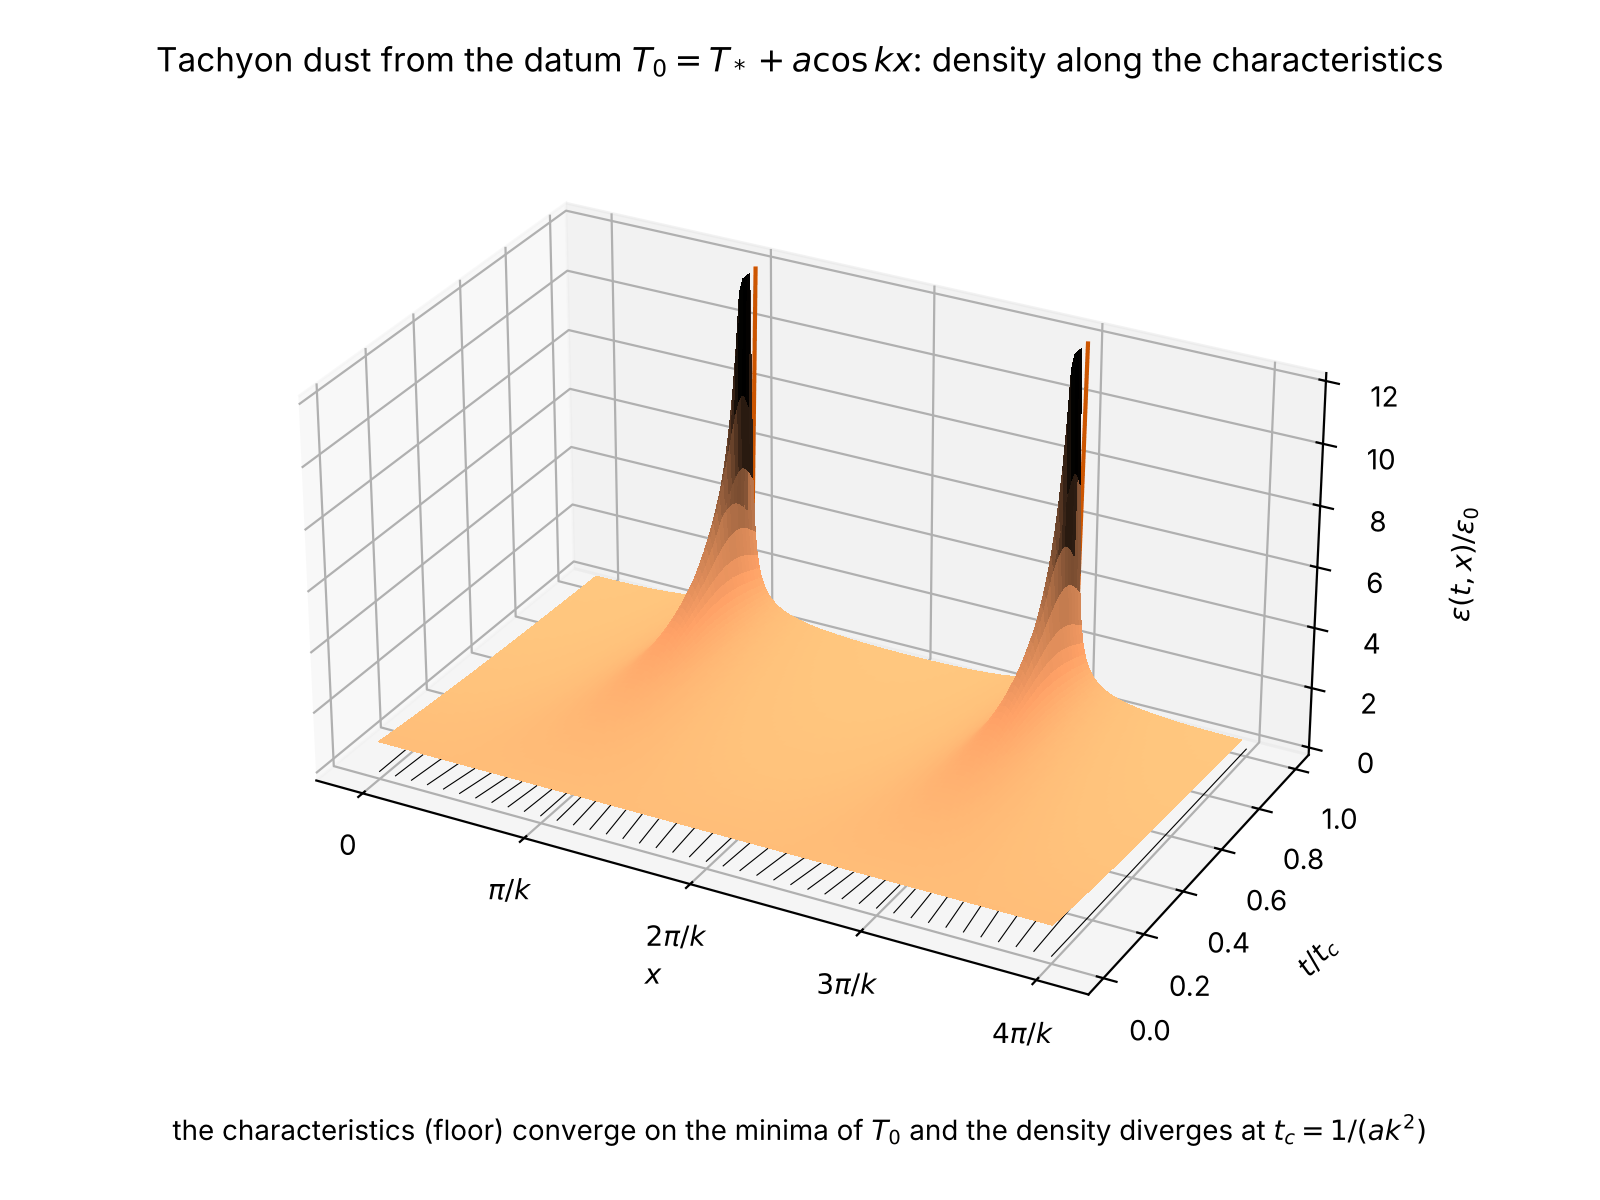
\includegraphics[width=\columnwidth]{figures/fig_caustic.png}
\caption{The dust of Theorem~\ref{thm:caustic} for the datum $T_0 = T_* + a\cos kx$ of Appendix~\ref{app:dust}, with $a = 1/2$, $k = 1$. The characteristics, drawn on the floor, are straight lines that converge on the minima of $T_0$; the energy density along them is $\eps_0/(1 + t\,v_0'(x_0))$ and diverges at $t_c = 1/(ak^2)$, where the vertical lines stand. The surface is cut at twelve times the initial density.}
\label{fig:caustic}
\end{figure}

\begin{proof}
By Lemma~\ref{lem:dustflow}(iii) the eigenvalues of $Dv_0(x_0)$ are real, and are all nonnegative at $x_0$ exactly when $\nabla^2T_0(x_0)\succeq 0$. (i) If $T_0$ is convex this holds at every $x_0$, so $\det(I+tDv_0(x_0)) = \prod_k(1+t\lambda_k(x_0))\ge 1$ and is non-decreasing for $t\ge0$, and Lemma~\ref{lem:dustflow}(ii) gives $\eps(t,X(t;x_0))\le\eps_0(x_0)$, non-increasing in $t$. (ii) If $T_0$ is not convex there is $x_0$ at which $\nabla^2 T_0$ has a negative eigenvalue, hence $Dv_0(x_0)$ has an eigenvalue $\lambda<0$, and $\det(I+tDv_0(x_0))$ vanishes at $t = -1/\lambda$. The infimum of these first zeros over $x_0$ is $t_c = 1/\mu_-$ (with $t_c=0$ if $\mu_- = \infty$, which happens only for unbounded curvature). For $t<t_c$ the solution exists along every characteristic, and along a characteristic from a point $x_0$ at which the first zero is attained or approached, Lemma~\ref{lem:dustflow}(ii) gives $\eps(t,X(t;x_0)) = \eps_0(x_0)/\det(I+tDv_0(x_0))\to+\infty$ as $t\uparrow t_c$; if the supremum is only approached, the same holds along a sequence of characteristics. At $t_c$ the map $x_0\mapsto X(t_c;x_0)$ is not a local diffeomorphism, and for $t>t_c$ two characteristics carrying different velocities pass through the same point, so $v$, and therefore $\nabla T$, is not single valued. (iii) A convex function on $\RR^p$ that is bounded above is constant: along any line it is a convex function of one variable bounded above, hence constant. So a bounded non-constant $T_0$ is not convex. (iv) is (ii) with $P = (1+T_0'^2)^{-1}$ and $H = T_0''$. Appendix~\ref{app:dust} and Figure~\ref{fig:caustic} work out the time $t_c$ and the density profile for the perturbation $T_0 = a\cos kx$ of the homogeneous decay and compares them with the numerical solutions of \cite{FKS02}.
\end{proof}

\begin{verdict}[claim 17]
False as stated. Tachyon matter is the final state of homogeneous decay, by Theorem~\ref{thm:homogeneous}, and is not the final state of inhomogeneous decay: by Theorem~\ref{thm:caustic} the dust of \cite{Sen02field} reaches infinite density at a finite time $t_c$ for every initial profile that is bounded and not constant, and the equations stop describing anything after $t_c$. The caustics were found numerically in the full Born--Infeld equation \eqref{eq:dbi} by Felder, Kofman and Starobinsky \cite{FKS02}, who also derived the free-streaming approximation, and analytically for several tachyon effective actions by Barnaby \cite{Barnaby04} and Felder and Kofman \cite{FK04}; the theorem above is the exact statement for the dust limit of \cite{Sen02field}, with the convexity criterion and the time. What the caustic becomes in string theory is open: the effective action \eqref{eq:dbi} is derived for slowly varying fields and is not valid where second derivatives diverge, and the two candidates for the physics there, the formation of closed strings \cite{LLM07} and the appearance of higher-derivative corrections that smooth the fold, are not decided. Sen's review \cite{Sen04review} states the result for the homogeneous solution, which is what is proved; the general sentence of \cite{Sen02matter} is what we record as false.
\end{verdict}

\subsection{Closed string emission and open--closed duality}\label{ssec:emission}

The decaying brane couples to closed strings, and the question whether the classical open string description of Theorem~\ref{thm:homogeneous} survives their emission was raised in \cite{Sen02rolling} and answered in part by Lambert, Liu and Maldacena \cite{LLM07}: the energy radiated into closed strings by a decaying D$p$-brane is infinite at leading order for $p\le2$ and finite for $p>2$; for $p=0$ the divergence, cut off at energies of order $1/g_s$, carries away an energy of the order of the mass of the brane, so that all the energy of the brane goes into closed strings. Sen \cite{Sen03openclosed} turned this into the conjecture of \emph{open--closed duality at tree level}: the tree-level open string theory on the decaying brane, with its tachyon matter, is a dual description of the closed string state produced by the decay, so that the two are not to be added.

\begin{verdict}[claim 18]
Confirmed. The conjecture is supported by the computation of \cite{LLM07}, in which the closed string state produced is determined by the open string boundary state and its energy, for $p=0$, is the energy of the brane; by the matching of the energy-momentum tensor of the emitted closed strings with that of tachyon matter in the regime where both can be computed \cite{Sen03openclosed}; and by the two-dimensional string theory, where the decay of the D0-brane is the motion of a single fermion of the matrix model and the open and closed descriptions are provably the same \cite{Sen04review}. No proof exists in the critical string, and the missing step is a control of the backreaction of the emitted closed strings on the open string dynamics beyond leading order in $g_s$. The conjecture is stated for homogeneous decay; after Theorem~\ref{thm:caustic} the inhomogeneous case has no classical open string side to be dual to beyond $t_c$.
\end{verdict}

\section{Non-BPS branes and the descent relations}\label{sec:nonbps}

The tachyon conjectures of Section~\ref{sec:tachyon} have a static counterpart: the solitons of the tachyon field are themselves D-branes. Sen \cite{Sen98bab} identified the vortex on a D$p$--$\overline{\rm D}p$ pair of type II with the BPS D$(p-2)$-brane, \cite{Sen98spinor} identified the kink on a D1--$\overline{\rm D}$1 pair of type I with a stable non-BPS D-particle transforming as a spinor of $SO(32)$, the state required by the duality with the heterotic string, and \cite{Sen99descent} organised these into the \emph{descent relations}: the non-BPS D$p$-brane of type II is the orbifold of the D$p$--$\overline{\rm D}p$ pair by $(-1)^{F_L}$, and the BPS D$(p-1)$-brane is the kink on the non-BPS D$p$-brane.

\begin{theorem}[claims 19, 20]\label{thm:descent}
\begin{enumerate}[label=(\roman*),leftmargin=2em]
\item At the critical radius $R = \sqrt{2}$ (in units $\alpha'=1$) of a circle transverse to the brane pair, the tachyon kink on a D$p$--$\overline{\rm D}p$ pair of type II wrapped on the circle is an exactly marginal boundary deformation, and the boundary conformal field theory at the end of the deformation is that of a non-BPS D$(p-1)$-brane; the kink on the non-BPS D$p$-brane at $R=1$ is, in the same way, the BPS D$(p-1)$-brane.
\item The conserved charges of D-branes and of their tachyon solitons are classified by the K-theory of spacetime: $K(X)$ for type IIB, $K^{-1}(X)$ for type IIA, $KO(X)$ for type I; the kink on the type I D1--$\overline{\rm D}$1 pair carries the class generating $KO^{-1}({\rm pt}) = \ZZ_2$ and is the $SO(32)$ spinor, stable and non-BPS.
\end{enumerate}
\end{theorem}

\begin{proof}
(i) is the construction of \cite{Sen98spinor,Sen99descent}: the tachyon of the wrapped pair at the critical radius has a vertex operator $\cos(X/\sqrt2)\otimes\sigma_1$ which is exactly marginal, the deformation by it can be followed to its end by fermionising the boson $X$, and the boundary state at the end is the boundary state of the lower brane with Dirichlet condition on $X$. (ii) is Witten's theorem \cite{Witten98K}, which starts from Sen's identification of the brane--antibrane system with a pair of bundles $(E,F)$ and the tachyon with a map between them and identifies the charge with the class of $(E,F)$ in K-theory; the type I computation $KO^{-1}({\rm pt})=\ZZ_2$ gives the $\ZZ_2$ charge of the spinor, which prevents its decay.
\end{proof}

\begin{verdict}[claims 19, 20]
Proved. Both statements are theorems of boundary conformal field theory and of K-theory respectively; the existence of the spinor as a stable non-BPS state was confirmed by its mass at weak coupling, which matches the heterotic spinor's at strong coupling up to the expected corrections, and by the identification of the stable non-BPS states of other orbifolds and orientifolds by the same method \cite{Sen99nonBPS}.
\end{verdict}

\begin{proposition}[claim 21; Sen 2003]\label{prop:kinkdbi}
In the effective action \eqref{eq:dbi} on a non-BPS D$p$-brane, the kink solution $T(x) = \lim_{a\to\infty} a\,x$ (a step of infinite slope) is singular as a field and regular as a source: its energy-momentum tensor is $\mathcal T_{p-1}$ times a delta function at $x=0$, and the effective action of its collective coordinates and world-volume gauge field is exactly the Dirac--Born--Infeld action of a BPS D$(p-1)$-brane, to all orders in the fields and for every potential $V$ with $\int V\,dT$ finite. The same holds for the vortex on the brane--antibrane pair.
\end{proposition}

\begin{proof}
\cite{Sen03kink}, Sections~3 and~4: for the ansatz $T = f(a(x-\xi(y)))$ with $f$ odd and increasing, in the limit the action evaluated on the ansatz is independent of the profile $f$ and of the scale $a$, by the change of variables $T = f(\cdot)$, and equals $-\mathcal T_{p-1}\int\sqrt{-\det(g_{\alpha\beta}+F_{\alpha\beta})}$ with the induced metric of the embedding $\xi$; the equations of motion of the ansatz follow from the full equations because the action is stationary in $f$ and $a$.
\end{proof}

\begin{verdict}[claim 21]
Proved, within the effective action. The statement is about \eqref{eq:dbi} and is exact there; it says nothing about the string theory corrections to \eqref{eq:dbi}, which are not controlled on the kink, where second derivatives are large. The agreement of the tension and of the form of the world-volume action with those of the D$(p-1)$-brane is the content of the claim and holds.
\end{verdict}

\section{The Sen limit of F-theory}\label{sec:senlimit}

Sen \cite{Sen96ftheory} showed that F-theory on an elliptic K3 surface, at the point of its moduli space where the Weierstrass model $y^2 = x^3 + f(z)x + g(z)$ has constant modulus $\tau$ and four $D_4$ singular fibres, is the type IIB orientifold on $T^2/\ZZ_2$ with four orientifold seven-planes and four D7-branes on each, with gauge group $SO(8)^4$ and constant coupling; and that moving away from this point, in a one-parameter family $f = -3h^2 + \eps\eta$, $g = -2h^3 + \eps h\eta - \tfrac{1}{12}\eps^2\chi$ with $\eps\to0$, the coupling becomes weak away from the loci $h=0$, which are the orientifold planes, while the discriminant $\Delta = -9\eps^2 h^2(\eta^2 - h\chi) + O(\eps^3)$ places the D7-branes on $\eta^2 = h\chi$. In \cite{Sen97orientifold} the same expansion was applied to F-theory on elliptic Calabi--Yau threefolds and fourfolds over a base $B$, with $h,\eta,\chi$ sections of $K_B^{-2}, K_B^{-4}, K_B^{-6}$: the statement is that F-theory on such a Calabi--Yau has a weak coupling limit which is type IIB on the double cover of $B$ branched along $h=0$, with the orientifold projection, O7-planes on $h=0$ and D7-branes on $\eta^2=h\chi$.

\begin{theorem}[scope of the weak-coupling expansion]\label{thm:senlimitk3}
For $f=-3h^2+\eps\eta$ and $g=-2h^3+\eps h\eta-\eps^2\chi/12$, one has
\begin{align}
4f^3+27g^2={}&-9\eps^2h^2(\eta^2-h\chi)\nonumber\\
&+\eps^3(4\eta^3-\tfrac92h\eta\chi)+\tfrac3{16}\eps^4\chi^2.
\end{align}
At points with $h(\eta^2-h\chi)\ne0$, the modular invariant $j\propto f^3/(4f^3+27g^2)$ diverges as $\eps^{-2}$. This is a generic-point limit, not a smooth elliptic fibration at $\eps=0$: its discriminant vanishes identically there. The perturbative orientifold and D7 interpretation is the construction in \cite{Sen96ftheory,Sen97orientifold}. The generic O7 monodromy is $-T^{-4}$ in the convention of \cite{Sen97orientifold}; the enhanced O7 with four coincident D7-branes has combined monodromy $-I$.
\end{theorem}
\begin{proof}
The discriminant identity follows by expansion; the leading nonzero coefficient gives the asserted growth. The two monodromies concern different configurations: adding the four D7 monodromies $T^4$ cancels the $T^{-4}$ factor. A Kodaira type cannot be read from the everywhere-degenerate central fibre as though it were an ordinary smooth family.
\end{proof}

\begin{verdict}[claim 22]
Established in the stated geometric and physical framework. The constant-coupling $SO(8)^4$ model and the generic weak-coupling family are related constructions, not identical fibre configurations.
\end{verdict}

\begin{proposition}[base divisor and double-cover divisor]\label{prop:senlimitcy}
Suppose $h,\eta$ are local coordinates near $h=\eta=0$ on a smooth base and $\chi$ is nonzero there. The divisor $D_B=\{\eta^2-h\chi=0\}$ on the base is smooth at that point. On the smooth orientifold double cover $X=\{\xi^2=h\}$ its pullback is
\[
D_X=\{\eta^2-\xi^2\chi=0\},
\]
which is singular along $\xi=\eta=0$. Where $\chi$ is a unit it has two local branches. At a transverse triple locus $\xi=\eta=\chi=0$ in a three-dimensional cover, its local equation is the Whitney pinch form $u^2=v^2w$.
\end{proposition}
\begin{proof}
For $F=\eta^2-h\chi$, at $h=\eta=0$ one has $dF=-\chi\,dh\ne0$. On the cover, the three derivatives of $G=\eta^2-\xi^2\chi$ in these coordinates are $2\eta,-2\xi\chi,-\xi^2$, all zero on the stated double locus. A unit $\chi$ has a local analytic square root, so $G=(\eta-\xi\sqrt\chi)(\eta+\xi\sqrt\chi)$. The transverse triple locus gives the pinch form. This is the distinction used in the D7 analysis of \cite{CDE09}.
\end{proof}

\begin{proposition}[a non-Higgsable divisor is not a sufficient obstruction]\label{prop:i0star}
In a local chart let $s=0$ be a divisor and take
\[
h=s h_1,\qquad\eta=s^2\eta_2,\qquad\chi=s^3\chi_3.
\]
Then $f=s^2F_\eps$, $g=s^3G_\eps$, with
\[
F_\eps=-3h_1^2+\eps\eta_2,\quad
G_\eps=-2h_1^3+\eps h_1\eta_2-\eps^2\chi_3/12.
\]
If the coefficients are generic units, the divisor has vanishing orders $(2,3,6)$ for nonzero $\eps$ and $j$ on it grows as $\eps^{-2}$ when $h_1(\eta_2^2-h_1\chi_3)\ne0$. Thus an $I_0^*$ divisor does not itself force strong coupling in the limit.
\end{proposition}
\begin{proof}
The common factor $s^6$ cancels in $f^3/(4f^3+27g^2)$, leaving Theorem~\ref{thm:senlimitk3} with $h_1,\eta_2,\chi_3$. This is a local calculation, not a global existence theorem on an arbitrary base. The allowed $I_0^*$ case is explicitly distinguished from exceptional-fibre obstructions in \cite{HLS18}.
\end{proof}

\subsection{Every weak coupling limit is Sen's}\label{ssec:normalform}

Sen's argument for the generality of his family is the following passage of \cite{Sen97orientifold}, after his equations~(4) and~(5), $f=C\eta-3h^2$ and $g=h(C\eta-2h^2)$:
\begin{quote}\small
``Since $\eta$ is an arbitrary polynomial (subject to the same restrictions as $f$, and its overall normalization specified separately in the constant $C$), we see from (4) that by choosing the most general $\eta$ and $C$ we can get the most general $f$. Thus we only need to deform $g$. To this end consider the following form of $g$: $g=h(C\eta-2h^2)+C^2\chi$ (21) where $\chi$ is a general polynomial subject to the same restrictions as $g$. This will certainly give us the most general $g$.''
\end{quote}
The limit is then $C\to0$ with $h,\eta,\chi$ fixed, and his equation~(23) gives $\Delta=-9C^2h^2(\eta^2+12h\chi)$; with $C=\eps$ and $\chi\to-\chi/12$ this is the family of Theorem~\ref{thm:senlimitk3}.\footnote{Sen's $\chi$ is $-\tfrac1{12}$ times the $\chi$ used here and in \cite{HLS18}; the D7 equation $\eta^2+12h\chi_{\rm Sen}=0$ of his~(23) becomes $\eta^2-h\chi=0$.} The passage shows that every Weierstrass model is a member of the family for some value of $C\ne0$. It does not show the converse that matters for the limit: that a family of Weierstrass models whose coupling becomes weak must approach the orientifold point along a path of this form. Theorem~\ref{thm:normalform} proves that converse.

Let $B$ be a normal projective variety and $L$ a line bundle on $B$; for a Calabi--Yau total space $L=K_B^{-1}$, which is Sen's equation~(29), $c_1(B)=c_1(L)$. A \emph{degeneration} is a pair of formal power series
\[
f_\eps\in H^0(B,L^4)[[\eps]],\qquad g_\eps\in H^0(B,L^6)[[\eps]],\qquad \Delta_\eps=4f_\eps^3+27g_\eps^2\not\equiv0,
\]
regarded as a Weierstrass curve over the field $K(B)((\eps))$, with $j_\eps=1728\cdot4f_\eps^3/\Delta_\eps$. It is \emph{weakly coupled} if $j_\eps\to\infty$ at the generic point of $B$, that is, if $v(j_\eps)<0$ for the $\eps$-adic valuation $v$ of $K(B)((\eps))$.\footnote{In the language of elliptic curves over a discretely valued field, the curve has potentially multiplicative reduction \cite[Prop.~VII.5.5]{Silverman09}; $\operatorname{Im}\tau\sim-v(j)\log|\eps|/2\pi$, so the string coupling $g_s=1/\operatorname{Im}\tau$ goes to zero as $\eps\to0$.} Two degenerations are \emph{equivalent} if they differ by a base change $\eps=t^k$ and a rescaling $(f,g)\mapsto(t^{-4r}f,t^{-6r}g)$, $r\in\ZZ$, which is the isomorphism $(x,y)\mapsto(t^{-2r}x,t^{-3r}y)$ of Weierstrass curves and leaves $j$ unchanged.

\begin{theorem}[normal form of weak coupling]\label{thm:normalform}
\begin{enumerate}[label=(\roman*),leftmargin=2em]
\item Every weakly coupled degeneration is equivalent, through a base change $\eps=t^k$ with $k\in\{1,2,4\}$, to a family of Sen's form
\begin{equation}\label{eq:normalform}
f=-3h^2+t\,\eta_t,\qquad g=-2h^3+t\,h\,\eta_t-\tfrac1{12}t^2\chi_t,
\end{equation}
with $h\in H^0(B,L^2)$ nonzero and independent of $t$, $\eta_t\in H^0(B,L^4)[[t]]$ and $\chi_t\in H^0(B,L^6)[[t]]$.
\item Conversely, every family \eqref{eq:normalform} with $h\ne0$ and $\Delta\not\equiv0$ is weakly coupled, with $v(j)\le-2$.
\item The orientifold divisor is determined by the limit: if $(f_0,g_0)$ is the leading coefficient of the rescaled family, then $4f_0^3+27g_0^2=0$ and $h=3g_0/(2f_0)$.
\end{enumerate}
\end{theorem}

The proof, in Appendix~\ref{app:closures}, uses only the valuation of $j$ and the normality of $B$, which makes a rational section of $L^2$ whose square is regular itself regular. The $t$-dependence of $\eta_t$ and $\chi_t$ is the only difference from Sen's ansatz, and it does not change the leading data: by Theorem~\ref{thm:senlimitk3} the discriminant is $-9t^2h^2(\eta_0^2-h\chi_0)+O(t^3)$, so the O7-plane is $h=0$ and the D7-brane is $\eta_0^2=h\chi_0$ exactly as Sen states.\footnote{A family $f=-3h^2+tF_t$, $g=-2h^3+tG_t$ whose first-order term violates $G_0=hF_0$ has discriminant $108\,t\,h^3(hF_0-G_0)+O(t^2)$ and $v(j)=-1$; the base change $t=s^2$ in the proof brings it to the form~\eqref{eq:normalform}. This is the only source of the exponent $k=4$.}

\begin{corollary}[existence of a weak coupling limit]\label{cor:existence}
A weakly coupled degeneration over $B$ exists if and only if $H^0(B,L^2)\ne0$; for a Calabi--Yau total space, if and only if $h^0(B,-2K_B)>0$. If $h\ne0$ is a section of $L^2$, the family $\eta=h^2$, $\chi=0$ has
\[
\Delta=h^6t^2(4t-9),\qquad j=1728\cdot\frac{4(t-3)^3}{t^2(4t-9)},
\]
constant on $B$: it is the global weak coupling limit of \cite[Eqs.~(2.13)--(2.15)]{HLS18}.
\end{corollary}

The criterion is a property of the base alone, so it settles the existence question that Sen's paper leaves to the examples. It does not say that the limit is free of strongly coupled regions; that depends on the vanishing of $h$ along special curves.

\begin{proposition}[rigid curves of self-intersection at most $-5$]\label{prop:rigidcurves}
Let $B$ be a smooth surface, $L=K_B^{-1}$, and $C\subset B$ a smooth rational curve with $C^2=-n$.
\begin{enumerate}[label=(\roman*),leftmargin=2em]
\item Every section of $L^k$ vanishes on $C$ to order at least $\lceil k(n-2)/n\rceil$. For $n\ge5$ this gives $\operatorname{ord}_Cf\ge3$ and $\operatorname{ord}_Cg\ge4$.
\item If $n\ge5$ and, for a given $\eps\ne0$, the Weierstrass model is minimal along $C$, then the value of $j$ at the generic point of $C$ is $0$ or $1728$. Along a degeneration minimal along $C$ for $\eps\ne0$ the coupling on $C$ therefore stays of order one.
\item In every weakly coupled degeneration $h$ vanishes on $C$ to order at least $2$ if $n\ge5$, and at least $1$ if $n=3,4$.
\end{enumerate}
\end{proposition}

Part~(i) is the intersection argument of Morrison and Taylor \cite{MT12}, and part~(ii) restates for every $\eps$ the observation of Halverson, Long and Sung that fibres of types $IV^*$, $III^*$, $II^*$ carry a fixed coupling \cite[Table~1 and Section~2.1]{HLS18}. Part~(iii) is new as stated: it places every rigid curve of self-intersection $\le-3$ inside the orientifold locus. For $n=3,4$ it reproduces Proposition~\ref{prop:i0star}; for $n\ge5$ the branch divisor of the double cover is not reduced along $C$, so the cover is not normal there. On the Hirzebruch surface $\FF_{12}$, for instance, $h^0(-2K)=51$ and weak coupling exists at the generic point by Corollary~\ref{cor:existence}, but every section of $-2K$ vanishes doubly on the curve of self-intersection $-12$, where the fibre has type $II^*$ and $j=0$.\footnote{With the rays $(1,0),(0,1),(-1,12),(0,-1)$ of the fan of $\FF_{12}$, the curve of the ray $(0,1)$ has self-intersection $-12$, and the polygon of $-kK$ is $\{(a,b):a\ge-k,\ b\le k,\ 12b\ge a-k\}$. For $k=2$ it has $5+17+29=51$ lattice points, all with $b\ge0$, and the monomial of $(a,b)$ vanishes to order $b+2\ge2$ on the curve; for $k=4,6$ the least orders are $4$ and $5$, the fibre type $II^*$.}

\begin{corollary}[the orientifold double cover]\label{cor:k3cover}
Let $B$ be a smooth rational surface or an Enriques surface, $L=K_B^{-1}$, and let a weakly coupled degeneration be given in the form~\eqref{eq:normalform}. Let $X=\{\xi^2=h\}$ be the double cover of $B$ branched along $O=\{h=0\}$, with $\xi$ a section of $L$, Sen's equation~(18).
\begin{enumerate}[label=(\roman*),leftmargin=2em]
\item $K_X=\pi^*(K_B+L)=0$, which is Sen's equation~(30). If $O$ is reduced with at most simple singularities, $X$ has rational double points and its minimal resolution is a K3 surface.
\item If $B$ is an Enriques surface, $L^2$ is trivial, $h$ is a nonzero constant and $X$ is the K3 surface covering $B$. Then $f$ and $g$ are constants, there is no orientifold plane and no D7-brane, and the coupling is constant over $B$ for every $\eps$.
\item For general $h,\eta_0,\chi_0$ the D7 divisor $D_B=\{\eta_0^2=h\chi_0\}\in|{-8K_B}|$ is smooth and meets $O$ only at the $8K_B^2$ points $h=\eta_0=0$, where it is tangent to $O$. Its pullback $D_X$ has a node over each of these points, and the normalisation $\widetilde D\to D_B$ is an unramified double cover.
\item If $Y\to B$ is the smooth Weierstrass model, then
\[
\chi(Y)=-60K_B^2,\quad\chi(O)=-2K_B^2,\quad\chi(D_B)=-56K_B^2,\quad\chi(\widetilde D)=-112K_B^2,
\]
and $2\chi(Y)=4\chi(O)+\chi(\widetilde D)$.
\end{enumerate}
\end{corollary}

Part~(iv) is the two-dimensional case of the identity $2\chi(Y)=\chi(\overline D)+4\chi(O)-\chi(S)$ of Aluffi and Esole \cite[Cor.~4.7]{AE09}, in which the pinch locus $S$ is empty because three general sections $h,\eta_0,\chi_0$ have no common zero on a surface; here it follows from the adjunction formula and a count of the cusps of the discriminant. Part~(iii) shows that the singularity of Proposition~\ref{prop:senlimitcy} is, on a surface, a set of nodes, and the Whitney pinch first appears for threefold bases.

\begin{figure}[tbp]
\centering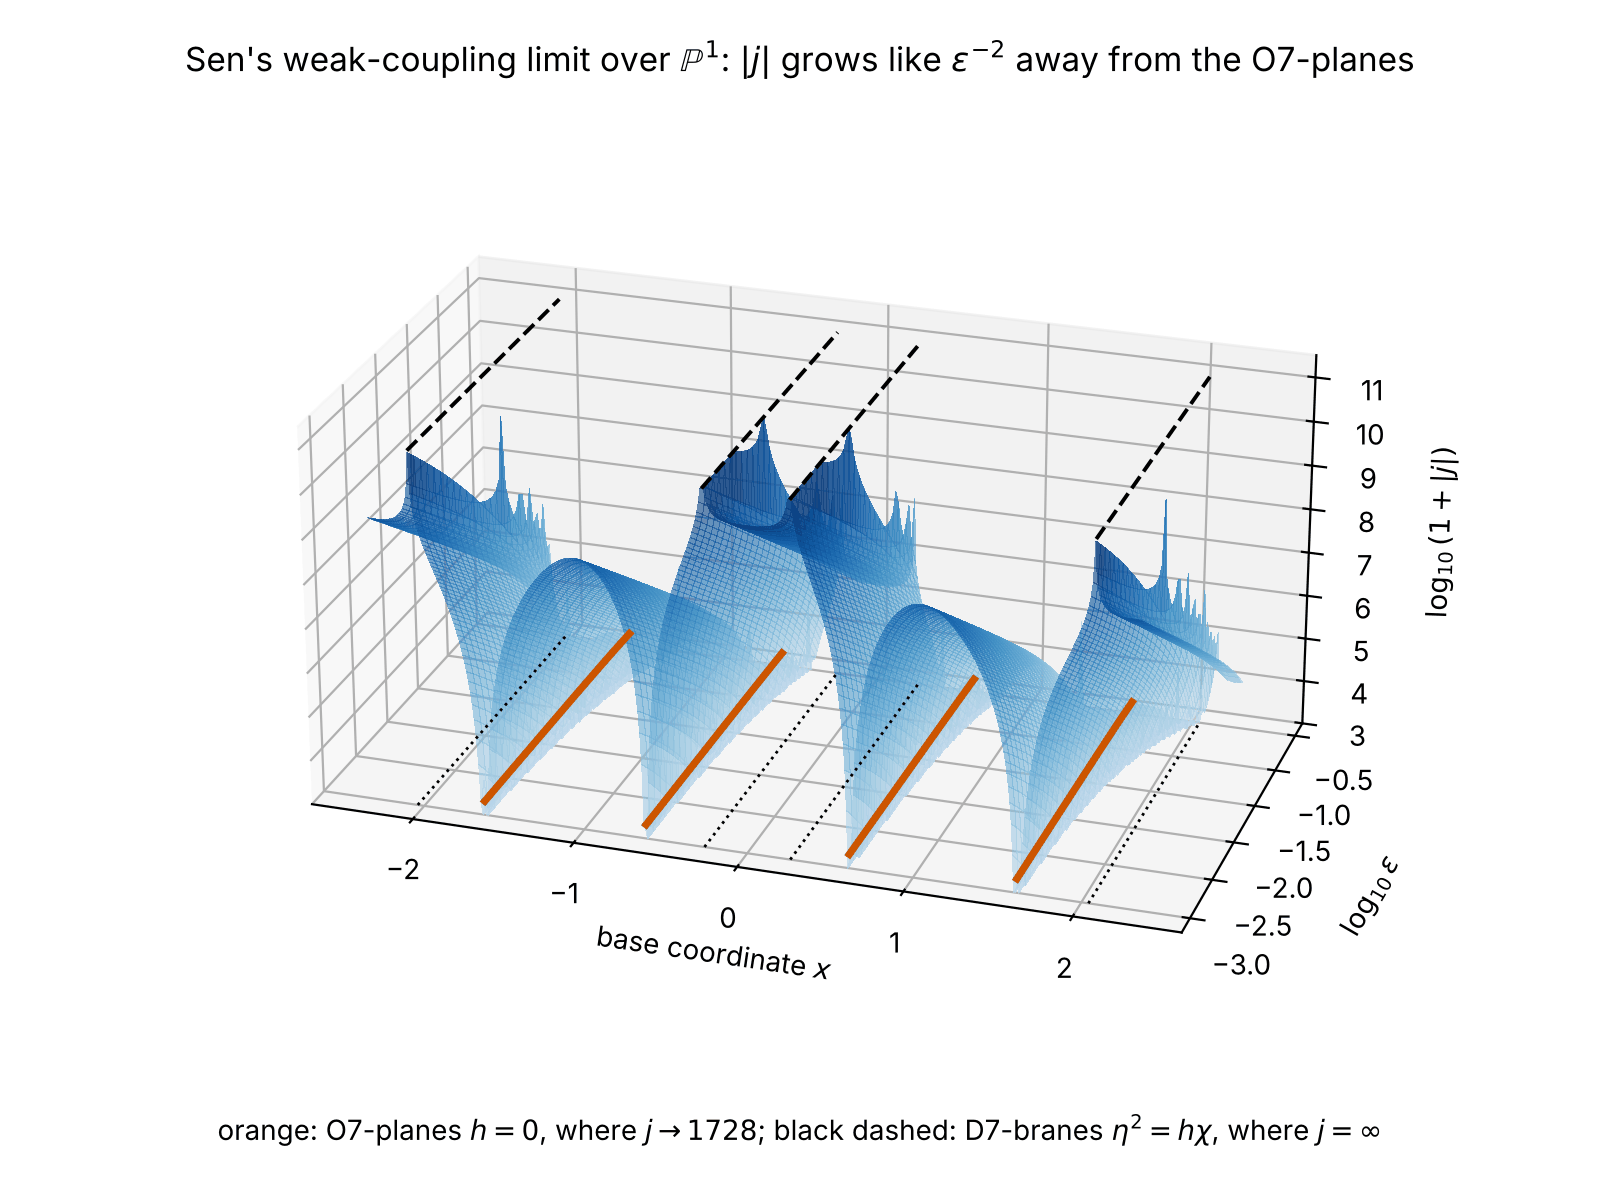
\includegraphics[width=0.94\linewidth,height=0.46\textheight,keepaspectratio]{figures/fig_weakcoupling.png}
\caption{Sen's K3 limit as a surface over the base coordinate $x$ of $\PP^1$ and the parameter $\eps$: the height is $\log_{10}(1+|j|)$ for $h=x^4-3x^2+1$, $\eta=x^8+2$, $\chi=3x^{12}+5$, sections of $L^2,L^4,L^6$ with $L=\mathcal O(2)$; values below $10^3$ are drawn on the floor. The coupling becomes weak, $|j|\sim\eps^{-2}$, everywhere except at the four O7-planes $h=0$ (orange lines), where $j\to1728$, and the four real D7-branes $\eta^2=h\chi$ (dashed), where $j$ has a pole for every $\eps$.}
\label{fig:weakcoupling}
\end{figure}

\begin{verdict}[claim 23]
Proved, in the form of Theorem~\ref{thm:normalform}: up to base change and rescaling, every weak coupling degeneration of F-theory on an elliptic Calabi--Yau is Sen's family, with the O7 divisor $h=0$ fixed by the limit point, and such a degeneration exists exactly when $h^0(-2K_B)>0$ (Corollary~\ref{cor:existence}). Sen calls the reduction formal and says that the auxiliary manifold can be singular; Proposition~\ref{prop:rigidcurves} and Corollary~\ref{cor:k3cover} identify when it is. Rigid curves of self-intersection $\le-5$ keep the coupling of order one and force a non-reduced branch divisor, and on surfaces the D7 singularity is a set of nodes. The physical identification of the limit with a type~IIB orientifold, beyond the geometry and the monodromies of Theorem~\ref{thm:senlimitk3}, remains a statement of string theory and is not proved here.
\end{verdict}

\section{Black hole entropy: the entropy function and small black holes}\label{sec:entropy}

\subsection{The entropy function}\label{ssec:entropyfunction}

For an extremal black hole in a theory of gravity with covariant higher-derivative terms in the framework specified below, whose near-horizon geometry has the symmetry $SO(2,1)\times SO(D-1)$ of $AdS_2\times S^{D-2}$ with electric fields $e_i$ and magnetic charges $p_a$, Sen \cite{Sen05entropy} defined the entropy function
\begin{equation}\label{eq:entropyfunction}
\begin{gathered}
\mathcal E(\vec u,\vec v,\vec e,\vec q,\vec p) = 2\pi\big(e_i q_i - f(\vec u,\vec v,\vec e,\vec p)\big),\\
f = \int_{S^{D-2}}\sqrt{-\det g}\,\mathcal L ,
\end{gathered}
\end{equation}
where $f$ is the Lagrangian density integrated over the sphere on the near-horizon ansatz with radii $v_1,v_2$ of $AdS_2$ and $S^{D-2}$ and constant scalars $u_s$.

\begin{theorem}[claims 24, 25]\label{thm:entropyfunction}
\begin{enumerate}[label=(\roman*),leftmargin=2em]
\item The equations of motion of the near-horizon geometry are the conditions
\[
\partial\mathcal E/\partial u_s = \partial\mathcal E/\partial v_{1,2} = 0,\qquad \partial\mathcal E/\partial e_i = 0,
\]
the last being the definition of the charges $q_i$, and the Wald entropy of the black hole is the value of $\mathcal E$ at the extremum \cite{Sen05entropy}.
\item For rotating extremal black holes, whose near-horizon geometry has the symmetry $SO(2,1)\times U(1)$ and depends on the polar angle through functions $\Omega(\theta),\psi(\theta),\dots$, the same holds with $\mathcal E$ a functional of these functions and with an additional term $2\pi\alpha J$ for the angular momentum, the extremisation being over the functions as well as the constants \cite{AGJST06}.
\end{enumerate}
\end{theorem}

\begin{proof}
The derivation, including the normalization and curvature-variation convention, is given in \cite[Section~2]{Sen05entropy} and its rotating extension in \cite{AGJST06}. For a covariant Lagrangian with no derivatives of curvature, the Wald expression is $-2\pi\int_H (\partial\mathcal L/\partial R_{\mu\nu\rho\sigma})\epsilon_{\mu\nu}\epsilon_{\rho\sigma}$ with the induced volume factor and $\epsilon_{\mu\nu}\epsilon^{\mu\nu}=-2$. Curvature derivatives require the corresponding variational derivative, and Chern--Simons terms require separate treatment. The near-horizon equations and the Legendre transform give the entropy function in this framework. Local extremisation does not by itself construct a regular solution extending to prescribed asymptotic data.
\end{proof}

\begin{verdict}[claims 24, 25]
Proved. The theorem is a derivation within classical higher-derivative gravity with the stated symmetry; the attractor mechanism, that the entropy is independent of the asymptotic moduli, is a corollary whenever the extremum is isolated in the scalars. The results agree with the earlier supergravity computations of Cardoso, de Wit and Mohaupt where both apply \cite{Sen05entropy}, and the formalism has been used in every later comparison of macroscopic and microscopic entropies.
\end{verdict}

\subsection{Small black holes}\label{ssec:small}

A half-BPS state of the heterotic string on $T^6$ with winding $w$ and momentum $n$ on a circle, with $nw>0$, has $d_h(nw)\sim e^{4\pi\sqrt{nw}}$ states, while the two-derivative supergravity solution with these charges has a singular horizon of zero area. Sen \cite{Sen04stretch} argued that the higher-derivative terms stretch the horizon to string scale and that the entropy function with the Gauss--Bonnet term, $\mathcal L \supset \frac{1}{16\pi G}\phi(S)\big(R_{\mu\nu\rho\sigma}^2 - 4R_{\mu\nu}^2 + R^2\big)$ with the one-loop coupling $\phi(S)$, gives
\begin{equation}\label{eq:small}
S_{\rm BH} = 4\pi\sqrt{nw}
\end{equation}
in four dimensions, in agreement with the statistical entropy to leading order; \cite{Sen05stretching} extended the computation to the heterotic string in $D$ dimensions.

Sen states the outcome of the computation of \cite{Sen05stretching} in its abstract:
\begin{quote}\small
``The black hole entropy computed this way is finite and has the right dependence on the charges in accordance with the general scaling argument, but the overall numerical factor does not agree with that computed from the statistical entropy except for $D=4$ and $D=5$. This is not surprising in view of the fact that we do not use a fully supersymmetric action in our analysis; however this analysis demonstrates that higher derivative corrections are capable of stretching the horizon of a small black hole in arbitrary dimensions.''
\end{quote}
His result is \cite[Eq.~(3.20)]{Sen05stretching}, with the Gauss--Bonnet coefficient $C$ of his~(3.14),
\begin{equation}\label{eq:sen320}
S_{\rm BH}=a\sqrt{nw},\qquad a=\pi\sqrt C\sqrt{\frac{2}{(D-2)(D-3)}}\,\big\{8(D-2)(D-3)-4(D-4)(D-5)\big\}^{1/2}.
\end{equation}
Prester \cite{Prester06} then showed that the Lovelock action with the coefficients $\lambda_m=4^{1-m}/m!$ of his equation~(4.27) has, in every dimension, a near-horizon solution with $S_{\rm BH}=4\pi\sqrt{nw}$, and that his solution is unique for $D\le9$ \cite[footnote~9]{Prester06}. The rest of this subsection makes these statements exact for every dimension.

\paragraphx{The two-charge horizon.} We use the normalisation of \cite[Eq.~(4.3)]{Prester06}, with $n_D=D-2$ the dimension of the sphere and $\alpha'=1$ unless $\alpha'$ is written. The near-horizon geometry is $AdS_2\times S^{n_D}$ with squared radii $v_1,v_2$, the string-frame dilaton is $u_S$, the radius of the circle is $u_T$, and $e_1,e_2$ are the electric fields of the momentum and winding charges $q_1=2n/\sqrt{\alpha'}$, $q_2=2w/\sqrt{\alpha'}$. For a tree-level action whose higher-derivative terms are built from the Riemann tensor alone,
\begin{equation}\label{eq:fgeneral}
f=K\,u_S\,v_1v_2^{n_D/2}\Big[\frac{2(u_T^2e_1^2+e_2^2u_T^{-2})}{v_1^2}+Q(v_1,v_2)\Big],
\end{equation}
where $K>0$ is a constant and $Q$ is the curvature Lagrangian on the product of radii $v_1,v_2$; for the Einstein term $Q=n_D(n_D-1)/v_2-2/v_1$.

\begin{theorem}[entropy of the two-charge horizon]\label{thm:twocharge}
Let $R(v_1,v_2)=-v_1^2\,Q(v_1,v_2)$. The near-horizon solutions with $v_1,v_2,u_S,u_T,e_i>0$ are in bijection with the critical points of $R$ in the positive quadrant at which $R>0$, and at such a point
\begin{equation}\label{eq:sR}
S_{\rm BH}=4\pi\sqrt{nw}\,\sqrt{R_*/\alpha'}.
\end{equation}
In particular the black hole entropy equals the statistical entropy $4\pi\sqrt{nw}$ if and only if $R_*=\alpha'$, which is the condition $e_1e_2=\alpha'/4$ of \cite[Eq.~(5.6)]{Prester06}.
\end{theorem}

The proof is in Appendix~\ref{app:closures}. The theorem reduces the comparison with the statistical entropy, for every action of this class, to a single number: the critical value of a function of two variables. For the Lovelock actions $\mathcal L=\sum_m\lambda_m\alpha'^{m-1}\mathcal L_m^{GB}$ with $\lambda_1=1$ the function \eqref{eq:fgeneral} is that of \cite[Eq.~(4.3)]{Prester06}, and
\begin{equation}\label{eq:GH}
Q=H(v_2)-\frac{G(v_2)}{v_1},\quad G(y)=\sum_{m\ge1}\frac{2m\lambda_m\,n_D!}{(n_D+2-2m)!}\,y^{1-m},\quad H(y)=\sum_{m\ge1}\frac{\lambda_m\,n_D!}{(n_D-2m)!}\,y^{-m},
\end{equation}
the sums running over the terms with nonnegative factorial arguments.

\begin{corollary}[Lovelock actions]\label{cor:lovelock}
For a Lovelock action the near-horizon solutions correspond to the critical points $y$ of $\Phi=G^2/H$ on the set where $G>0$ and $H>0$, with $v_2=\alpha'y$, $v_1=\alpha'G/(2H)$ and $S_{\rm BH}=2\pi\sqrt{nw\,\Phi(y)}$. The statistical value is $\Phi=4$.
\end{corollary}

\begin{corollary}[the Gauss--Bonnet truncation in closed form]\label{cor:gb}
For $\lambda_2=1/8$ and $\lambda_m=0$ for $m\ge3$, with $a=(D-2)(D-3)$ and $b=(D-4)(D-5)$, there is exactly one near-horizon solution in every dimension $D\ge4$. It has $v_2=\alpha'(a-b)/4$, $v_1=2v_2/a$ and
\begin{equation}\label{eq:gbratio}
\frac{S_{\rm BH}}{4\pi\sqrt{nw}}=\sqrt{1-\frac{(D-4)(D-5)}{2(D-2)(D-3)}}.
\end{equation}
The ratio is $1$ for $D=4,5$, it is $\sqrt{11/12}$, $\sqrt{17/20}$, $\sqrt{4/5}$ for $D=6,7,8$, and it decreases to $1/\sqrt2$ as $D\to\infty$. It is the ratio $a_D/a_4$ of Sen's coefficients \eqref{eq:sen320}, for every value of $C$.
\end{corollary}

The corollary turns Sen's statement into a formula with its domain: the Gauss--Bonnet truncation fixes the horizon in every dimension, the entropy is below the statistical value for every $D\ge6$, and it never falls below $1/\sqrt2$ of it.\footnote{Sen prints \eqref{eq:sen320} with $C=1$ beside it, while his~(3.15) gives $C=1/8$ for the heterotic string; the two differ by the choice of $\alpha'$. Since $a\propto\sqrt C$, the ratio $a_D/a_4$ does not depend on this choice, and $a_4=4\pi$ by Sen's own statement fixes the normalisation.} The solution is the minimum of $\Phi$, and the critical point equation is linear in $1/y$, which is why it can be solved in every dimension.

\begin{theorem}[Prester's completion in every dimension]\label{thm:prester}
Let $\lambda_m=4^{1-m}/m!$ for every $m\ge1$, and $D\ge4$.
\begin{enumerate}[label=(\roman*),leftmargin=2em]
\item $H=2(G-2)$ identically, in every dimension. Equivalently $f$ has the form \cite[Eq.~(5.3)]{Prester06}.
\item On the line $v_1=\alpha'/2$ one has $R(\alpha'/2,v_2)=\alpha'$ for every $v_2$, and every near-horizon solution lies on this line. Hence every solution has $S_{\rm BH}=4\pi\sqrt{nw}$.
\item The near-horizon solution is unique: $v_2=\alpha'y_D$ with $y_D$ the only positive root of $H(y)=4$. Equivalently $I_{n_D}\big(1/(2y_D)\big)=2$, where
\[
I_N(t)=\sum_{m\ge0}\binom{N}{2m}(2m-1)!!\,t^m
\]
counts the involutions of an $N$-element set with weight $t$ per transposition, or again $i^{-n_D}\operatorname{He}_{n_D}\big(i\sqrt{2y_D}\big)=2(2y_D)^{n_D/2}$ with $\operatorname{He}_N$ the Hermite polynomial.
\item As $D\to\infty$, with $n_D=D-2$,
\[
y_D=\frac{n_D^2}{4\ln2}-\frac{(2\ln2+1)\,n_D}{4\ln2}+O(1).
\]
\end{enumerate}
\end{theorem}

Part~(ii) for one solution is Prester's argument of \cite[Section~5]{Prester06}, which he gives without solving for $v_2$; parts~(i) and~(ii) show that it applies to every solution, because $\partial_{v_2}R=v_1G'(v_2)(1-2v_1)$ and $G'<0$. Part~(iii) extends his uniqueness statement from $D\le9$ to every dimension, and part~(iv) refines the leading term $v_2\to D^2\alpha'/(4\ln2)$ of \cite[Eq.~(20)]{Prester13}. The first values are $y_4=1/2$, $y_5=3/2$, $y_6=3/2+\sqrt3$, and $y_{40}=489.273\dots$

\begin{theorem}[the coefficients are forced]\label{thm:rigidity}
Fix $D\ge4$, let $m=\lfloor D/2\rfloor$, and take $\lambda_k=4^{1-k}/k!$ for $k<m$ and $\lambda_m=\beta\,4^{1-m}/m!$ with $\beta>0$.
\begin{enumerate}[label=(\roman*),leftmargin=2em]
\item The coefficient $\lambda_m$ enters $G$ and not $H$, and $\Phi_\beta=G_\beta^2/H$ attains its minimum on $(0,\infty)$.
\item If $\beta>1$, every near-horizon solution has $S_{\rm BH}>4\pi\sqrt{nw}$.
\item If $\beta<1$, the solution at the minimum of $\Phi_\beta$ has $S_{\rm BH}<4\pi\sqrt{nw}$.
\end{enumerate}
Consequently, if $\lambda_1=1$, every $\lambda_k$ is positive, and the solution at the minimum of $\Phi$ has the statistical entropy in every dimension, then $\lambda_k=4^{1-k}/k!$ for every $k$.
\end{theorem}

The induction in the last statement uses that $\lambda_m$ is the top coefficient both in $D=2m$ and in $D=2m+1$: it is fixed by $D=2m$, and Theorem~\ref{thm:prester} shows that the same value works in $D=2m+1$. This proves the statement of \cite{Prester13} that the matching ``fixes the coefficients $\lambda_k$ to the form (6) uniquely'', which there rests on the computations of \cite{Prester06}. Figures~\ref{fig:valley} and~\ref{fig:rigidity} show the two mechanisms: a line of constant $R$ on which every solution lies, and a minimum that crosses the statistical value only at $\beta=1$.

\begin{figure}[tbp]
\centering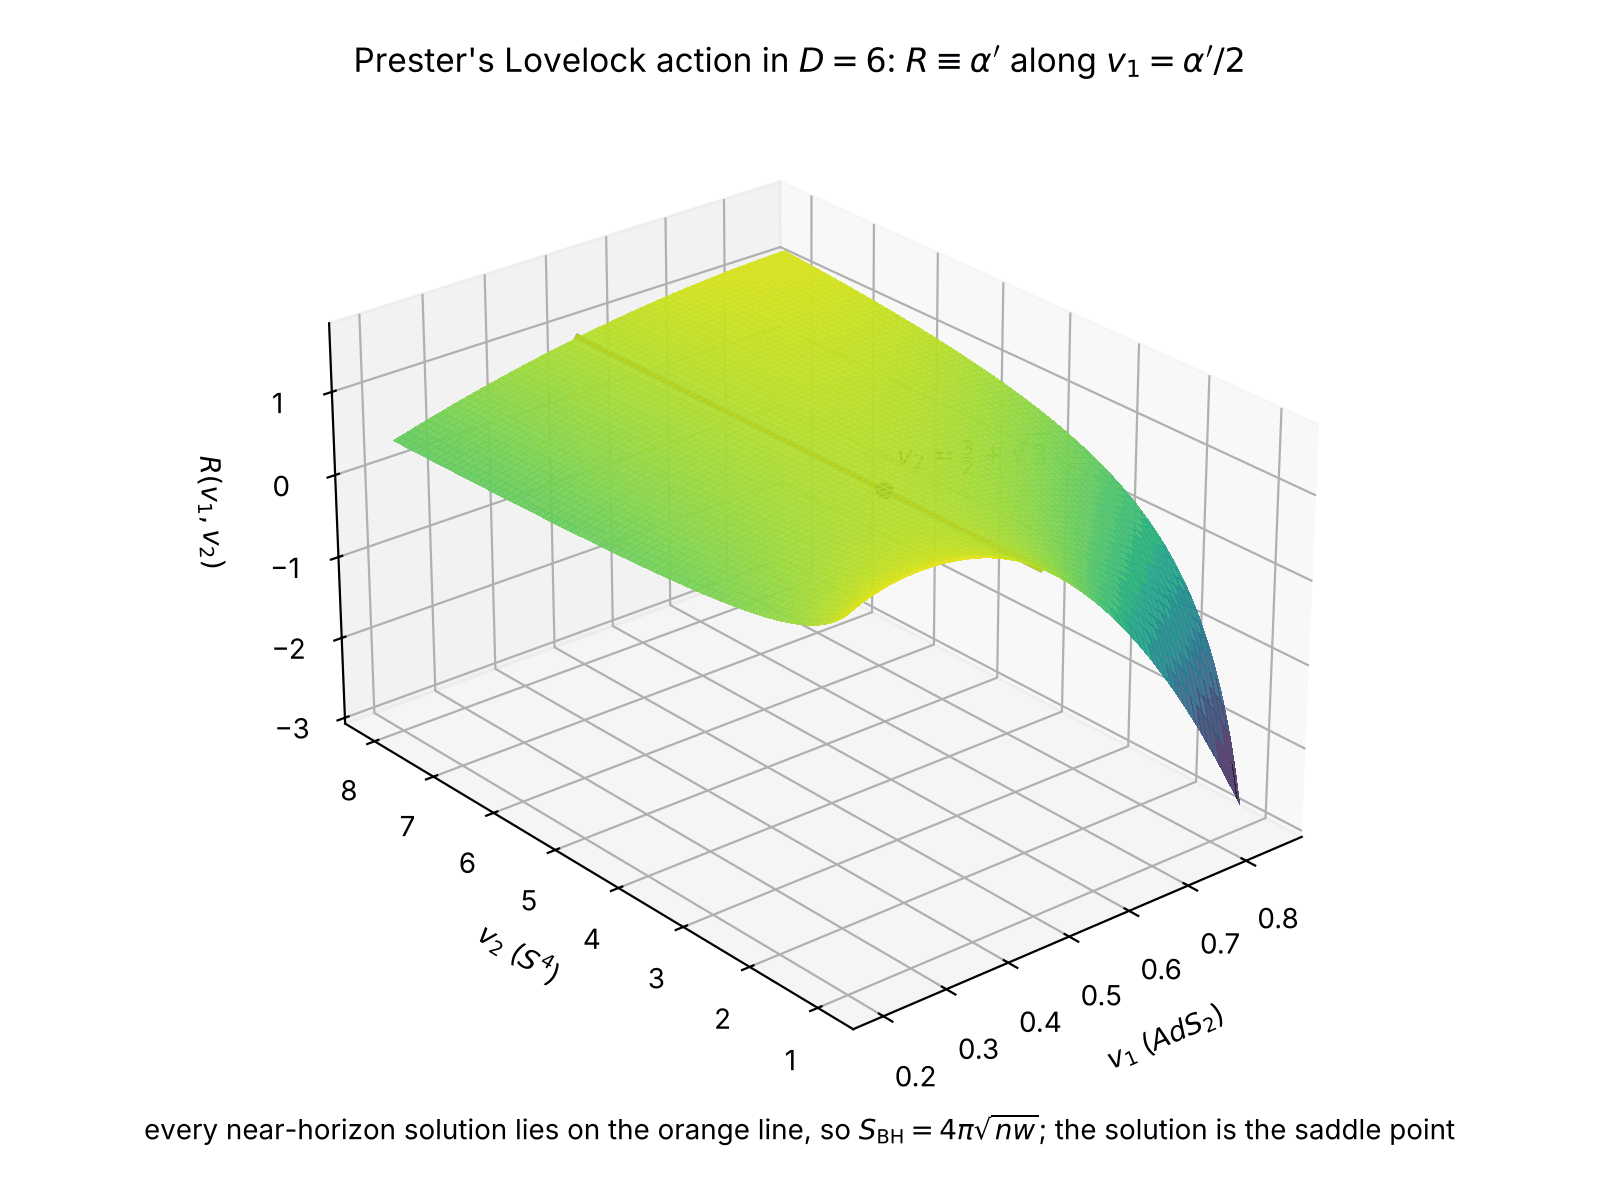
\includegraphics[width=0.94\linewidth,height=0.46\textheight,keepaspectratio]{figures/fig_valley.png}
\caption{The function $R(v_1,v_2)$ of Theorem~\ref{thm:twocharge} for Prester's coefficients in $D=6$, in units $\alpha'=1$. Along the line $v_1=1/2$ (orange) the surface has the constant height $R=1$, the value that gives $S_{\rm BH}=4\pi\sqrt{nw}$; the near-horizon solution is the saddle point on this line, at $v_2=3/2+\sqrt3$.}
\label{fig:valley}
\end{figure}

\begin{figure}[tbp]
\centering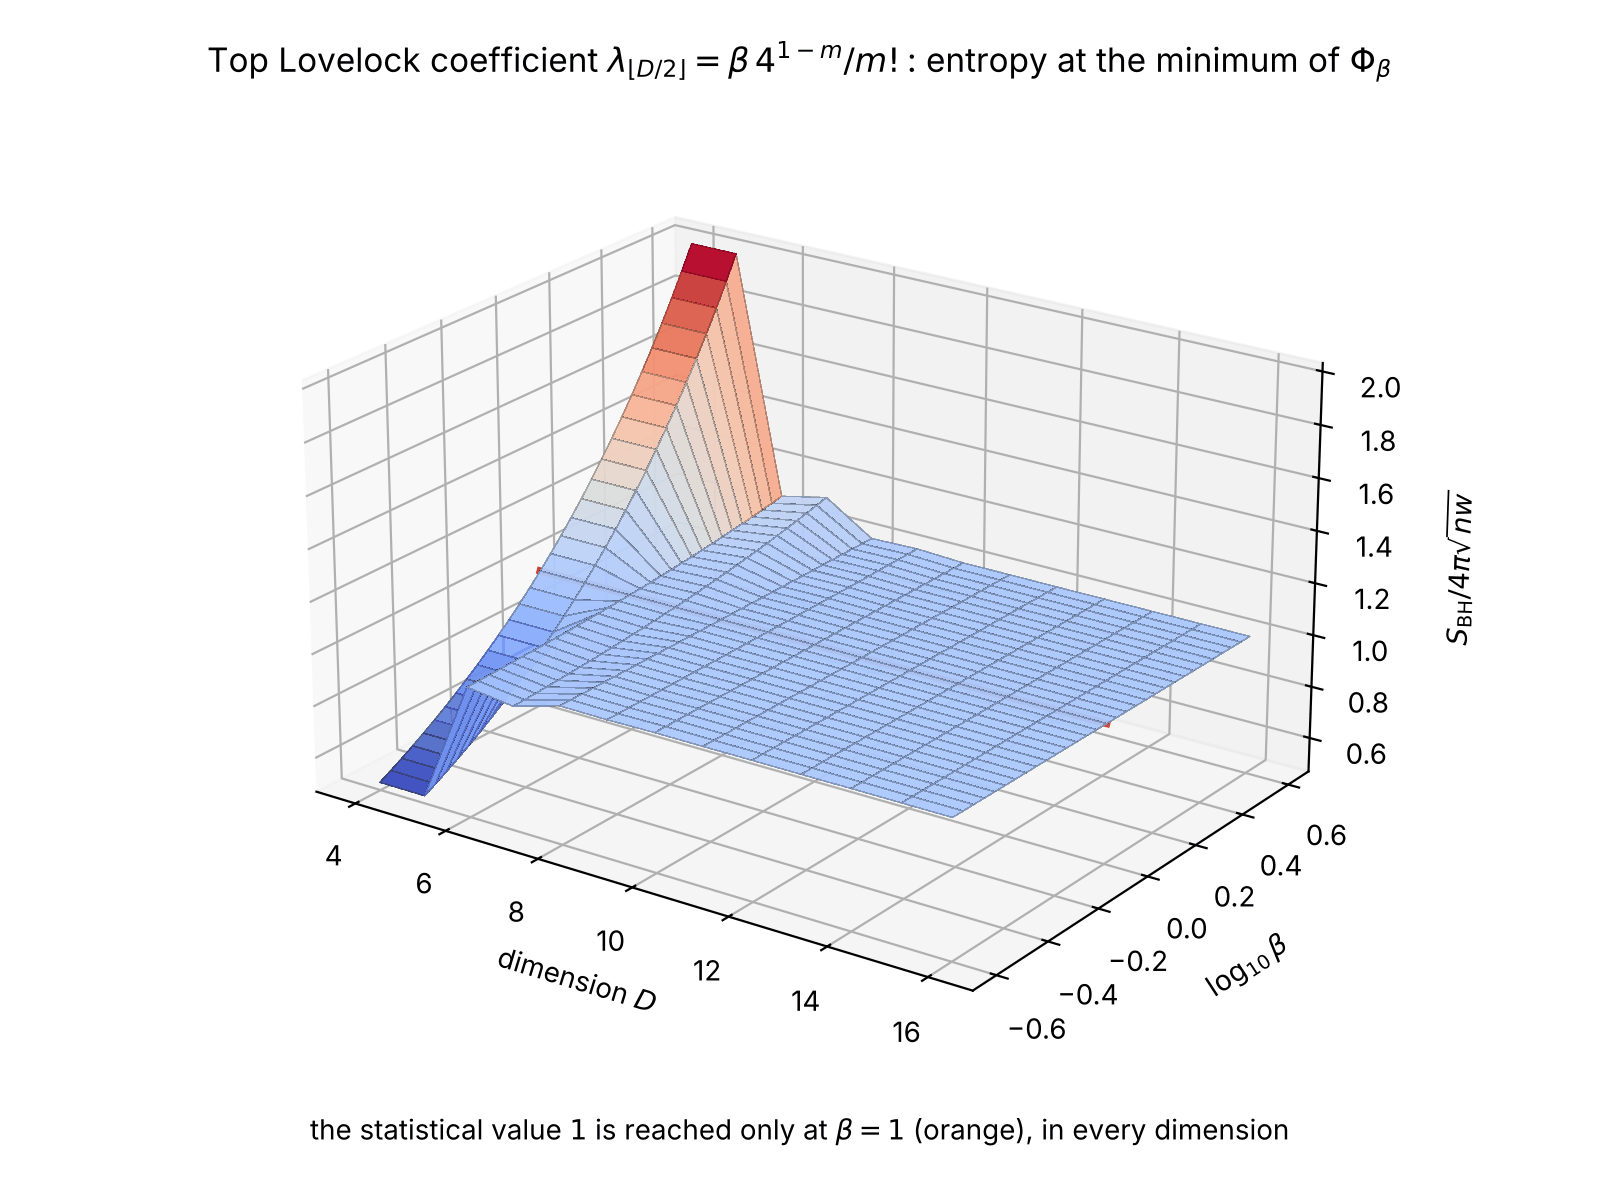
\includegraphics[width=0.94\linewidth,height=0.46\textheight,keepaspectratio]{figures/fig_rigidity.png}
\caption{The entropy at the minimum of $\Phi_\beta$, divided by $4\pi\sqrt{nw}$, as a surface over the dimension $D$ and the factor $\beta$ of the top Lovelock coefficient (Theorem~\ref{thm:rigidity}). The level $1$ is met only along $\beta=1$ (orange): above it the entropy exceeds the statistical value, below it the entropy falls short.}
\label{fig:rigidity}
\end{figure}

\begin{remark}[four dimensions]\label{rem:fourd}
In $D=4$ the agreement extends to all orders in $1/\sqrt{nw}$ when the supersymmetric $F$-terms are used in place of the Gauss--Bonnet term: \cite{Dabholkar05} evaluated the entropy with the full $F$-term, and \cite{DDMP05} matched it with the asymptotic expansion of $d_h$ up to non-perturbative terms. The Gauss--Bonnet term reproduces the leading term because on the near-horizon geometry the four-dimensional $F$-term reduces to it at this order.
\end{remark}

\begin{remark}[what remains open for the heterotic string]\label{rem:heterotic}
\gap{The heterotic effective action in $D\ge6$ is not the Lovelock action.} It contains no cubic Gauss--Bonnet density, its quartic terms carry $\zeta(3)$, and it has higher-derivative terms in the gauge fields \cite[Section~6]{Prester06} and gravitational Chern--Simons terms \cite[footnote~6]{Prester13}. Theorem~\ref{thm:twocharge} still applies to its pure-curvature part, so the open question is the single statement $R_*=\alpha'$ for the complete action on $AdS_2\times S^{D-2}$, and that requires the full $\alpha'$ expansion, which is not known. The holographic arguments of \cite{DM08,KLS07,LSS07}, which obtain the entropy from the central charge of an $AdS_3$ near-horizon region fixed by symmetries and anomalies, support the statistical value in every dimension; they do not compute $R_*$ from an action.
\end{remark}

\begin{verdict}[claim 26]
Proved, for the statements Sen makes. The Gauss--Bonnet truncation gives a finite horizon in every dimension, with the entropy \eqref{eq:gbratio} in closed form, equal to the statistical value exactly for $D=4,5$ (Corollary~\ref{cor:gb}). For every action whose corrections are built from curvature, the comparison is the single condition $R_*=\alpha'$ (Theorem~\ref{thm:twocharge}); Prester's Lovelock completion satisfies it with a unique solution in every dimension, and its coefficients are the only ones that do (Theorems~\ref{thm:prester} and~\ref{thm:rigidity}). The statement that the complete heterotic effective action gives $4\pi\sqrt{nw}$ in every $D\ge6$ remains open (Remark~\ref{rem:heterotic}).
\end{verdict}

\section{The quantum entropy function and the logarithmic corrections}\label{sec:quantum}

\subsection{The quantum entropy function}\label{ssec:qef}

Sen \cite{Sen08qef} proposed that the exact degeneracy of the horizon states of an extremal black hole with charges $\vec q$ is the finite part of the Euclidean string theory path integral on the near-horizon $AdS_2$,
\begin{equation}\label{eq:qef}
d_{\rm hor}(\vec q) = \Big\langle \exp\Big[-i q_i\oint A^{(i)}_\theta\, d\theta\Big]\Big\rangle^{\rm finite}_{AdS_2} ,
\end{equation}
with a Wilson line insertion at the boundary carrying the charges, the boundary conditions fixing the charges rather than the chemical potentials, and the ``finite part'' defined by subtracting the terms proportional to the length of the boundary; and that this quantity matches the appropriately signed horizon index for quarter-BPS black holes after hair removal and the helicity-trace convention are fixed (Section~\ref{ssec:hair}).

\begin{verdict}[claim 27]
Confirmed. The proposal passes every test that can be computed: the classical limit of \eqref{eq:qef} is the exponential of the Wald entropy; the one-loop correction is the logarithmic term, which matches the microscopic index exactly in $\mathcal N=4$ and $\mathcal N=8$ (Theorem~\ref{thm:logs}); and the localisation of the path integral in $\mathcal N=2$ supergravity, proposed in \cite{BBGMS10} and carried out in \cite{DGM11,DGM13}, reproduces the exact Rademacher expansion of the index of $\mathcal N=8$ black holes and the leading Bessel function of the $\mathcal N=4$ one \cite{MurthyReys16,IMT25,IMT25b}. The last of these results is weaker than its statement in the literature, and Sen's own later assessment \cite{Sen23localisation} says so: \gap{the claim that supersymmetric localisation of the $AdS_2$ path integral reproduces the Rademacher expansion from first principles} rests on three steps that are not established. The Killing spinors of the near-horizon geometry grow at the boundary of $AdS_2$ and do not act on the space of normalisable fluctuations over which the path integral is defined, so the localisation argument has no proved domain; the measure on the localisation manifold used in \cite{DGM11,MurthyReys16} is postulated and not derived, and a different measure changes every subleading term; and the one-loop determinants over the transverse directions depend on an ultraviolet cut-off that the computation sets, without justification, at the four-dimensional Planck scale. Sen himself discusses these qualifications in \cite{Sen23localisation}; they are not counted here as errors left unacknowledged by him. There is no proof: the path integral is not defined beyond the semiclassical expansion, the localisation argument assumes an off-shell supersymmetric completion of the higher-derivative terms, and the identification of the subtracted terms with the hair is made case by case. The missing step is a definition of the right-hand side of \eqref{eq:qef} that does not rely on a saddle point expansion; the conjecture is, in this sense, a proposal for what that definition should give.
\end{verdict}

\subsection{The logarithmic corrections}\label{ssec:logs}

The one-loop contribution to \eqref{eq:qef} from the massless fields on $AdS_2\times S^2$ gives a term $c\ln A_H$ in the entropy, with $c$ determined by the spectrum and the two-derivative action alone. Banerjee, Gupta, Mandal and Sen \cite{BGMS11} computed it for quarter-BPS black holes in $\mathcal N=4$ and eighth-BPS black holes in $\mathcal N=8$ string theory, and Sen \cite{Sen12N2} for half-BPS black holes in $\mathcal N=2$ theories with $n_V$ vector and $n_H$ hypermultiplets.

\begin{theorem}[claim 28]\label{thm:logs}
The logarithmic correction to the entropy of a quarter-BPS black hole in any $\mathcal N=4$ string compactification is zero, and that of an eighth-BPS black hole in $\mathcal N=8$ string theory on $T^6$ is $-4\ln A_H$. Both agree with the microscopic indices: the asymptotic expansion of the Fourier coefficients of $1/\Phi_{10}$ and its CHL analogues has no logarithmic term, and that of the $\mathcal N=8$ index, a Fourier coefficient of $\vartheta_1(\tau,z)^2/\eta(\tau)^6$, has the term $-2\ln\Delta$ with $\Delta\propto A_H^2$, that is, $-2\ln\Delta = -4\ln A_H$ \cite{BGMS11}.
\end{theorem}

\begin{proof}
The macroscopic computation is the heat kernel of the quadratic fluctuation operator of all massless fields on $AdS_2\times S^2$ with the near-horizon flux, including the graviton, the gravitini and the vector fields, with the zero modes of the asymptotic symmetries treated separately; the coefficient is the $s^0$ term of the heat kernel together with the zero-mode counting, $-(c_{\rm local} + c_{\rm zm})\ln a$ with $a$ the radius. In $\mathcal N=4$ the contributions cancel between the gravity multiplet and the vector multiplets \cite[Section~7]{BGMS11}; in $\mathcal N=8$ the net result is $-8\ln a = -4\ln A_H$ \cite[Section~8]{BGMS11}. The microscopic expansions are in \cite[Section~2]{BGMS11}, from the saddle point expansion of the inverse Siegel form \cite{DavidSen06} and of the Jacobi form. The computation was rederived from the on-shell action of the Euclidean solution and from the $AdS_2$ Schwarzian in \cite{IMT25,IMT25b}, with the same coefficients.
\end{proof}

\begin{verdict}[claim 28]
Proved, as a match between two computations each of which is complete: the macroscopic coefficient is a theorem of one-loop quantum field theory on the near-horizon geometry and the microscopic one of the asymptotics of modular forms. The rotating black holes in four and five dimensions \cite{Sen12rotating} and the extremal Kerr and Reissner--Nordstr\"om black holes without supersymmetry \cite{Sen12N2,Sen13schwarzschild}, for which no microscopic count exists, are predictions and remain confirmed in the sense of claim~29.
\end{verdict}

\begin{proposition}[claim 29; Sen 2012]\label{prop:n2log}
For a half-BPS black hole in an $\mathcal N=2$ supergravity with $n_V$ vector and $n_H$ hypermultiplets, the logarithmic correction is $\frac{1}{12}(23 + n_H - n_V)\ln A_H$, equal to $\big(2 - \frac{\chi}{24}\big)\ln A_H$ with $\chi = 2(n_V - n_H + 1)$ the Euler number of the Calabi--Yau threefold in the type IIA convention, with the universal hypermultiplet included; the type IIB Euler-number relation has the opposite sign.
\end{proposition}

\begin{proof}
\cite{Sen12N2}, by the same heat kernel method, the only difference from $\mathcal N=4$ being the absence of the cancellation; the result was rederived by \cite{KLL14} from the heat kernel of $\mathcal N=2$ supergravity on the same background.
\end{proof}

\begin{verdict}[claim 29]
Confirmed. A universal comparison for the full class of $\mathcal N=2$ theories is not established here; this does not deny microscopic indices in particular $\mathcal N=2$ compactifications. The comparison made in \cite{Sen12N2} is with the measure in the OSV formula, and agrees with the measure proposed by Denef and Moore if their result is extrapolated to weak topological string coupling. A model-independent microscopic comparison in a fixed ensemble is not established here.
 The general framework and the ensemble must be fixed before comparing a logarithmic coefficient.
\end{verdict}

\subsection{A check of the cutoff-scale preprint}

The current preprint \cite{Sen26cutoff} separates the extended-supergravity cancellation from an unresolved nonzero-Euler-number case. There is a local notation problem in its Eq.~(2.7): a contribution to $\Delta\ln Z_n$ is printed as the multiplicative factor $(g_s^{-1}\lambda_S^2)^2$. In the logarithm it must instead read
\begin{equation}
\Delta\ln Z_{\rm rot}=\ln[(g_s^{-1}\lambda_S^2)^2]
=-2\ln g_s+4\ln\lambda_S.
\end{equation}
This is a notation correction, not a refutation of the later result. Combining this expression with the three translational modes, the fermionic modes, two-form modes and the ensemble terms gives the stated coefficients $(\alpha_{NZ}+7-n)$ and $(n_{NS}-4)$ in its Eq.~(2.10). The elementary coefficient sums are checked in the analytic supplement. The current arXiv PDF was inspected for this equation; the INSPIRE record checked for this revision supplied no journal-version or erratum metadata. That search result is not a proof that no correction exists elsewhere.

The cutoff comparison in \cite{Sen26cutoff} keeps other inputs fixed. Its Section~4 explicitly allows coordinated changes of duality frame and measure, and its Section~5 leaves the $\chi\ne0$ discrepancy unresolved. These qualifications prevent the conditional cutoff calculation from being restated as a theorem excluding every other ultraviolet completion. We do not claim to solve its Calabi--Yau discrepancy here.

\section{String field theory, D-instantons, soft theorems and matrix theory}\label{sec:sft}

\subsection{String field theory}\label{ssec:sft}

Two claims of Sen about string field theory itself are in the catalogue. The first, with Zwiebach \cite{SenZwiebach94}, is that closed string field theory is background independent under infinitesimal deformations of the conformal field theory: the string field theories formulated around two nearby conformal backgrounds are related by a field redefinition. The second is the construction of superstring field theory \cite{Sen15offshell,Sen15onePI,Sen16BV} and the proof of its unitarity \cite{Sen16unitarity}: a gauge-invariant one-particle-irreducible effective action for heterotic and type II strings, free of the divergences of the picture-changing operators of earlier formulations through the use of a second, free string field of picture number $-3/2$; a Batalin--Vilkovisky master action; and the cutting rules, hence unitarity, of the resulting amplitudes.

\begin{verdict}[claims 30, 31]
Proved. Claim~30 is proved in \cite{SenZwiebach94} for marginal deformations to first order (and to second order in the companion paper), by constructing the field redefinition from the connection on the space of conformal field theories; its extension to finite deformations is a theorem only within the formal perturbation theory of the string field and is not a claim of the paper. Claim~31 is a construction and is proved in the papers that make it: the 1PI action is gauge invariant by the main identity of the vertices, the master action satisfies the master equation, and the Cutkosky rules are derived in \cite{Sen16unitarity} with the $i\epsilon$ prescription of \cite{Pius16}. The reader who wants the construction in one place has the review \cite{SenZwiebach24}. None of this depends on a conjecture; the open questions of superstring field theory are not about these statements.
\end{verdict}

\paragraphx{Corrected versions and infrared scope.} The published erratum to \cite{Pius16} and the corrected arXiv v3 must be used for the cutting argument; the correction is excluded from the list of unresolved errors. Section~4 of \cite{Sen16unitarity} explicitly notes the infrared problem for $D\le4$ and that the inclusive-cross-section construction is not carried out there. This is an acknowledged limitation, not a hidden failure of its perturbative cutting proof. A simple leading-soft cancellation and a counterexample to inferring exact unitarity from a formal series are given in Appendix~\ref{app:perturbative}. Appendix~\ref{app:infraredlimit} constructs the finite-energy limit in the explicit positive soft model and states the additional string-amplitude estimate needed for transfer. Appendix~\ref{app:softremainder} derives a uniform subtracted tree-emission bound from Sen's soft theorem and demonstrates why overlapping limits require additional estimates. None of these is a construction of the full infrared-finite string S-matrix.

\subsection{D-instantons}\label{ssec:instantons}

The contribution of D-instantons to string amplitudes has an overall normalisation that the world-sheet theory does not fix, because the open string path integral on the instanton has zero modes, bosonic and fermionic, whose measure is ambiguous. Sen \cite{Sen20fixing,Sen21normalisation,Sen21IIB} showed that open string field theory fixes it: the zero modes are treated by changing variables from the string field to the collective coordinates with a Jacobian computed in the field theory, the gauge zero mode of the $U(1)$ on the instanton is handled by a gauge fixing that the field theory provides, and the resulting normalisation is finite and unambiguous.

\begin{verdict}[claim 32]
Confirmed. In two-dimensional string theory the normalisation computed this way \cite{Sen20fixing,Sen21Dinst} agrees with the matrix model to the order compared, including the two-instanton contribution \cite{BRY23}; in type IIB string theory in ten dimensions the normalisation of the D-instanton correction to the four-graviton amplitude \cite{Sen21IIB} agrees with the coefficient predicted by $SL(2,\ZZ)$ invariance, the Green--Gutperle Eisenstein series. The claim that string field theory fixes the normalisation in every background is confirmed by these cases and \gap{not proved in general}: the construction requires the string field theory of the instanton to be well defined, which it is in these examples, and a general statement needs a general treatment of the zero modes of the Ramond sector, which is not established by the examples discussed here.
\end{verdict}

\subsection{Soft theorems}\label{ssec:soft}

Laddha and Sen \cite{LaddhaSen19} proved the classical soft graviton theorem in dimensions $D>4$, the statement that the low-frequency gravitational radiation from a scattering process is determined by the momenta and angular momenta of the incoming and outgoing objects, including the sub-subleading term, directly from the classical equations \cite{Sen18subsub}; and Sahoo and Sen \cite{SahooSen19} found that in $D=4$ the soft expansion acquires logarithmic terms, $\ln\omega$ at the subleading order, whose coefficients are again universal, and conjectured the form of the corresponding quantum terms.

\begin{verdict}[claims 33, 34]
Claim~33 is proved: the classical theorem in $D>4$ is derived in \cite{LaddhaSen19}, and the classical logarithmic terms in $D=4$ in \cite{SahooSen19}, from the classical equations of motion with the long-range forces included. Claim~34 is confirmed: the quantum logarithmic terms were computed at one loop in \cite{SahooSen19} for scalar matter coupled to gravity and to electromagnetism and found to have the conjectured form, with the classical term and a quantum correction that depends only on the asymptotic momenta; the universality of the one-loop $\ln\omega$ terms was extended to spinning particles with the non-minimal couplings allowed by gauge and coordinate invariance by Krishna and Sahoo \cite{KrishnaSahoo23}, and the classical soft factors have been pushed to all orders in the electromagnetic case \cite{KKSS25}. \gap{It is not proved that the quantum $\ln\omega$ terms are one-loop exact}; the missing step is a proof that the two-loop and higher infrared divergences exponentiate in the way the conjecture requires; \cite{KrishnaSahoo23} states this as open, a complete higher-loop argument is not supplied here.
\end{verdict}

\paragraphx{A recent scope check.} The all-orders classical analysis of \cite{KKMSS26} distinguishes the Newtonian result from its proposed relativistic extension. It also finds that a separate all-orders conjecture of Alessio, Di Vecchia and Heissenberg, consistent with two-particle scattering, does not hold for general initial or final states with at least three particles. This is not a counterexample to Sen's earlier subleading quantum result. The extension in \cite{KKMSS26} is explicitly conjectural and is recorded as an open construction, not a wrong proof.

\subsection{Matrix theory}\label{ssec:matrix}

Sen \cite{Sen98matrix} argued, independently of Seiberg \cite{Seiberg97}, that the matrix theory description of M-theory in the infinite momentum frame follows from the compactification of M-theory on a light-like circle, taken as a limit of a small space-like circle, and extended it to tori $T^n$: the theory of $N$ D0-branes on $T^n$ in a limit in which the torus and the string scale shrink. For $n\le 3$ the limit is a maximally supersymmetric Yang--Mills theory in $n+1$ dimensions; for $n=4,5$ it is the $(2,0)$ theory on $T^5$ and the little string theory on $T^5$ respectively; and for $n\ge6$ the limit is, as Sen states, ``a theory without an independent definition'', the degrees of freedom of the D0-branes not decoupling from gravity. The two statements H1 and H2 of the catalogue are these, and they are recorded without a verdict: the first is the Seiberg--Sen argument, which is a derivation within the assumptions of the infinite momentum frame and \gap{has no independent test for $n\ge 4$}; the second is \gap{a statement about a theory that is not defined}, and cannot be tested in any regime. We mention them because the paper is cited as a derivation of matrix theory and the reader should know that its content for $n\ge6$ is a limit of a non-decoupled system, as its author says.

\section{Conclusion}\label{sec:conclusion}

The selected catalogue contains results proved within specified frameworks and physical proposals with different degrees of support. The exact computations and analytic tests do not justify a count of ``fatal errors'' in an author's work. The toroidal negative full indices and their subsequent hair interpretation are already in the literature. The caustic calculation concerns the classical dust approximation and leaves the homogeneous rolling solution intact. The divisor singularity belongs to the orientifold cover, while a local $I_0^*$ family shows why non-Higgsability alone does not prohibit weak coupling.

The remaining questions are mathematical and physical construction problems: the full monopole $L^2$ statement beyond the cited cases, general hair identification, a controlled definition of the quantum entropy function, and extensions of the stated soft and string-field results. They are not resolved by the finite tables. A meaningful new criticism would require a precise original statement with all its hypotheses retained and a counterexample within those hypotheses. No new false proof by Sen meeting that criterion is established in this revision.

A reader who wants to repeat the computations of this paper will find them in the archive \cite{Bha26}, together with the Lean formalisation of the finite statements: the Fourier coefficients of Tables~\ref{tab:phi10} and~\ref{tab:tor2}, the wall-crossing identities of Theorem~\ref{thm:wallcrossing} and the twenty-one negative indices of Theorem~\ref{thm:positivityfails}, each computed inside the Lean kernel from the definitions of the theta functions. The catalogue and physical interpretations are not formalised by these certificates. Mathematical parts of such subjects can be formalised, but that work must not be inferred from a finite arithmetic check.


\appendix
\section{The computation of the Fourier coefficients}\label{app:computation}

The tables of this paper are Fourier coefficients of the inverse of the product \eqref{eq:product}, computed in exact rational arithmetic. We record the steps so that the numbers can be reproduced without the program, which is in the archive \cite{Bha26}.

\paragraphx{The genera.} The twisted elliptic genera are expanded in $q = e^{2\pi i\tau}$ and $y = e^{2\pi i z}$ from the theta functions $\theta_i(\tau,z)$ and $\eta(\tau)$ as $q$-series with coefficients in $\ZZ[y,y^{-1}]$, and the coefficients $c^{(r,s)}_b(4n-j^2)$ are read off from $\sum_{n,j} c^{(r,s)}_b(4n-j^2)\,q^n y^j$. For K3, $F^{(0,0)} = 8A$ with $A = \sum_{i=2}^4\theta_i(\tau,z)^2/\theta_i(\tau,0)^2$; for the $\ZZ_2$ CHL model the genera are $F^{(0,0)} = 4A$, $F^{(0,1)} = \tfrac43 A - \tfrac23 B\,E_2(\tau)$, $F^{(1,0)} = \tfrac43 A + \tfrac13 B\,E_2(\tau/2)$, $F^{(1,1)} = \tfrac43 A + \tfrac13 B\,E_2((\tau+1)/2)$, with $B = \theta_1(\tau,z)^2/\eta(\tau)^6$ and $E_2(\tau) = 2E(2\tau)-E(\tau)$, where $E$ is the Eisenstein series of weight two normalised to $1 - 24\sum_{n\ge1}\sigma_1(n)q^n$; for the $\ZZ_2$ toroidal orbifold they are \eqref{eq:tor2genera}. The arguments $\tau/2$ and $(\tau+1)/2$ are handled by expanding in $q^{1/2}$ with the sign $(-1)^n$ on the odd powers, so every series is a Laurent series in $x = q^{1/8}$, which is the smallest fractional power that occurs.

\paragraphx{The product.} Each factor $(1 - e^{2\pi i(k'\sigma + l\rho + jv)})^{-c}$ of $1/\Phit$ is expanded as a binomial series in the monomial $e^{2\pi i(k'\sigma + l\rho + jv)}$ to the order needed, and the factors are multiplied as polynomials in the three variables $e^{2\pi i\rho}$, $e^{2\pi i\sigma/N}$, $e^{2\pi iv}$ truncated at the exponents $Q^2/2\le L$, $NP^2/2\le K$ wanted in the tables. The exponent $c = \sum_s e^{2\pi i s l/N}c^{(r,s)}_b(4k'l-j^2)$ is an integer for $N\le 2$, where the root of unity is $\pm1$; for $N=3,5,7$ it would require cyclotomic arithmetic, and we have not computed those models. The one factor with $k'=l=0$, $(1 - e^{\mp 2\pi iv})^{-2}$ after the prefactor is taken into account, is the only one whose expansion depends on the chamber: in the chamber $\operatorname{Im} v<0$ it is expanded in powers of $e^{-2\pi iv}$, in the chamber $\operatorname{Im} v>0$ in powers of $e^{2\pi iv}$. The two expansions give the two columns of Table~\ref{tab:phi10} at $\pm Q\cdot P$, and their difference is the wall-crossing jump of Theorem~\ref{thm:wallcrossing}, which the program checks for every $Q^2,P^2\in\{2,4,6\}$ and $|Q\cdot P|\le 4$.

\paragraphx{The index.} The coefficient of $e^{2\pi i(\rho Q^2/2 + \sigma P^2/2 + v\,Q\cdot P)}$ in $1/\Phit$, multiplied by $(-1)^{Q\cdot P+1}$, is the index $d(Q,P)$ of \eqref{eq:dvv}. For the orbifolds the prefactor of the product is $e^{2\pi i(\rho + \sigma/N + v)}$ for the CHL models and $e^{2\pi i(\rho + v)}$ for the toroidal orbifolds, as in \cite{CD19}, and the integral over $\sigma$ runs over a period of length $N$ (Remark~\ref{rem:normalisation}).

\paragraphx{The tables.} Table~\ref{tab:phi10} is the heterotic index for $Q^2,P^2\in\{2,4,6\}$ and $-2\le Q\cdot P\le 4$; it reproduces Table~1 of \cite{Sen11positivity} entry by entry. Table~\ref{tab:tor2} is the index of the $\ZZ_2$ toroidal orbifold for $Q^2\le 12$, $P^2\in\{0,2,4\}$ and $Q\cdot P\in\{0,1,2\}$; it agrees with Tables~17 to~19 of \cite{CD19} where they overlap and extends them from $Q^2 = 8$ to $Q^2 = 12$. Table~\ref{tab:violations} lists the charges in the cone \eqref{eq:z2conditions} with $Q^2\le 12$, $P^2\le 8$, $Q\cdot P\le 4$ whose index is negative. The same scan over the cone of the heterotic string and of the $\ZZ_2$ CHL model, up to $Q^2\le 12$ (heterotic) or $NQ^2/2\le 6$ (CHL), $P^2\le 6$, $Q\cdot P\le 4$, finds no non-positive index, and the CHL values reproduce Table~2 of \cite{Sen11positivity}.

\begin{table*}[t]
\centering\small
\setlength{\tabcolsep}{5pt}
\begin{tabular}{@{}cc*{7}{r}@{}}
\toprule
$Q^2$ & $P^2$ & \multicolumn{7}{c}{$d(Q,P)$ for $Q\cdot P = -2,\,-1,\,0,\,1,\,2,\,3,\,4$}\\
\midrule
2 & 2 & -209\,304 & 130\,329 & 50\,064 & 25\,353 & 648 & 327 & 0 \\
4 & 2 & -2\,023\,536 & 1\,598\,376 & 1\,127\,472 & 561\,576 & 50\,064 & 8\,376 & -648 \\
6 & 2 & -15\,493\,728 & 16\,844\,421 & 16\,491\,600 & 8\,533\,821 & 1\,127\,472 & 130\,329 & -15\,600 \\
4 & 4 & -16\,620\,544 & 28\,698\,000 & 32\,861\,184 & 18\,458\,000 & 3\,859\,456 & 561\,576 & 12\,800 \\
6 & 4 & -53\,249\,700 & 474\,507\,528 & 632\,078\,672 & 392\,427\,528 & 110\,910\,300 & 18\,458\,000 & 1\,127\,472 \\
6 & 6 & 2\,857\,656\,828 & 11\,890\,608\,225 & 16\,193\,130\,552 & 11\,232\,685\,725 & 4\,173\,501\,828 & 920\,577\,636 & 110\,910\,300 \\
\bottomrule
\end{tabular}
\caption{The index $d(Q,P) = (-1)^{Q\cdot P+1}c(Q,P)$ of quarter-BPS dyons of the heterotic string on $T^6$, from $1/\Phi_{10}$, in the chamber $\operatorname{Im} v<0$ (the expansion in powers of $e^{-2\pi i v}$). The table agrees entry by entry with Table~1 of \cite{Sen11positivity}. Entries with $Q\cdot P<0$ are the other chamber's values at $|Q\cdot P|$ by the symmetry $v\mapsto -v$; their negativity for $Q\cdot P\le -1$ is the two-centred contribution of Theorem~\ref{thm:wallcrossing}.}
\label{tab:phi10}
\end{table*}

\begin{table*}[t]
\centering\footnotesize
\setlength{\tabcolsep}{4pt}
\begin{tabular}{@{}c*{9}{r}@{}}
\toprule
& \multicolumn{3}{c}{$Q\cdot P=0$} & \multicolumn{3}{c}{$Q\cdot P=1$} & \multicolumn{3}{c}{$Q\cdot P=2$}\\
\cmidrule(lr){2-4}\cmidrule(lr){5-7}\cmidrule(lr){8-10}
$Q^2$ & $P^2=0$ & $P^2=2$ & $P^2=4$ & $P^2=0$ & $P^2=2$ & $P^2=4$ & $P^2=0$ & $P^2=2$ & $P^2=4$ \\
\midrule
0 & 2 & 64 & 816 & 0 & 0 & -8 & 0 & 0 & 0 \\
1 & -12 & -224 & -1\,248 & 1 & 96 & 1\,968 & 0 & 0 & -12 \\
2 & 48 & 1\,152 & 18\,240 & -8 & -256 & 840 & 0 & 64 & 2\,592 \\
3 & -168 & -3\,392 & -10\,320 & 37 & 1\,376 & 34\,656 & -2 & -224 & 2\,432 \\
4 & 528 & 11\,520 & 200\,736 & -136 & -3\,840 & 16\,632 & 16 & 1\,152 & 43\,392 \\
5 & -1\,512 & -30\,336 & -55\,424 & 439 & 13\,152 & 343\,152 & -72 & -3\,392 & 33\,720 \\
6 & 4\,032 & 83\,968 & 1\,544\,832 & -1\,288 & -33\,536 & 171\,152 & 256 & 11\,520 & 414\,336 \\
7 & -10\,176 & -202\,560 & -179\,022 & 3\,503 & 92\,928 & 2\,476\,752 & -806 & -30\,336 & 302\,400 \\
8 & 24\,528 & 496\,512 & 9\,480\,000 & -8\,968 & -220\,672 & 1\,265\,256 & 2\,320 & 83\,968 & 2\,926\,080 \\
9 & -56\,796 & -1\,118\,496 & -155\,232 & 21\,854 & 540\,416 & 14\,545\,584 & -6\,200 & -202\,560 & 2\,049\,968 \\
10 & 127\,008 & 2\,521\,600 & 49\,523\,328 & -51\,080 & -1\,204\,992 & 7\,558\,560 & 15\,616 & 496\,512 & 16\,919\,712 \\
11 & -275\,544 & -5\,374\,656 & 2\,684\,560 & 115\,154 & 2\,711\,616 & 73\,540\,080 & -37\,508 & -1\,118\,496 & 11\,568\,000 \\
12 & 581\,952 & 11\,389\,440 & 228\,872\,064 & -251\,528 & -5\,741\,824 & 38\,736\,600 & 86\,544 & 2\,521\,600 & 84\,554\,880 \\
\bottomrule
\end{tabular}
\caption{The index $d(Q,P)$ of quarter-BPS dyons in the $\ZZ_2$ toroidal orbifold of type IIB on $T^6$, from the product formula for $1/\Phit_2$ with the twisted elliptic genera \eqref{eq:tor2genera}, in the chamber $\operatorname{Im} v<0$ and with the normalisation of Remark~\ref{rem:normalisation}. The entries agree with Tables~17, 18 and~19 of \cite{CD19} in their common range $Q^2\le 8$. The column $P^2=0$ lies outside the single-centred cone; its sign is $(-1)^{Q^2}$. The negative entries inside the cone are those of Table~\ref{tab:violations}.}
\label{tab:tor2}
\end{table*}


\section{The caustic for a periodic perturbation}\label{app:dust}

This appendix works out Theorem~\ref{thm:caustic} for the simplest inhomogeneous initial datum in one space dimension, a periodic perturbation of the homogeneous decay,
\begin{equation}\label{eq:cosdatum}
T_0(x) = T_* + a\cos kx,\qquad a>0,\ k>0 ,
\end{equation}
on the branch $\partial_t T>0$, and records the quantities that a numerical solution of the full equation \eqref{eq:dbi} can be compared with.

\paragraph*{Velocity and its derivative.} With $T_0' = -ak\sin kx$ and $W_0 = \sqrt{1+a^2k^2\sin^2kx}$,
\begin{equation}
v_0(x) = \frac{ak\sin kx}{\sqrt{1+a^2k^2\sin^2 kx}},\qquad
v_0'(x) = \frac{ak^2\cos kx}{(1+a^2k^2\sin^2kx)^{3/2}} .
\end{equation}
The dust moves away from the maxima of $T_0$ (where $\cos kx=1$ and $v_0'>0$, a rarefaction) and towards its minima (where $\cos kx = -1$ and $v_0' = -ak^2<0$).

\paragraph*{The caustic time.} The supremum of $-v_0'$ is attained at the minima $x_m = (2m+1)\pi/k$ of $T_0$, so by Theorem~\ref{thm:caustic}(iv)
\begin{equation}\label{eq:tccos}
\mu_- = \sup_x\bigl(-v_0'(x)\bigr) = ak^2, \qquad t_c = \frac{1}{a k^2} .
\end{equation}
The characteristics $X(t;x_0) = x_0 + t\,v_0(x_0)$ from a neighbourhood of $x_m$ converge on $x_m$, which is a fixed point of the flow, and have a singular differential there at $t_c$; for $t>t_c$ the map $x_0\mapsto X(t;x_0)$ folds over near $x_m$ and three characteristics pass through each point of a growing interval around it. The smaller the perturbation, the later the caustic, and no value of $a>0$ avoids it; the time is finite for every amplitude and every wavelength, and diverges only in the homogeneous limit $a\to0$ or in the long-wavelength limit $k\to0$ at fixed $a$.

\paragraph*{The density.} Along the characteristic from $x_0$,
\[
\eps\bigl(t,X(t;x_0)\bigr) = \frac{\eps_0(x_0)}{1+t\,v_0'(x_0)},\qquad \eps(t,x_m) = \frac{\eps_0(x_m)}{1 - t/t_c},
\]
and the density at the minimum diverges as $(t_c - t)^{-1}$. Near the caustic, for $x_0 = x_m + \xi$ with $\xi$ small,
\[
v_0'(x_0) = -ak^2\Bigl(1 - \tfrac{k^2\xi^2}{2}(1 + 3a^2k^2)+O(\xi^4)\Bigr),
\]
so at $t=t_c$ the linear term of $X(t_c;x_m+\xi) - x_m$ cancels and
\[
X(t_c;x_m+\xi) = x_m + c\,\xi^3 + O(\xi^5),\qquad c = \tfrac{k^2}{6}(1+3a^2k^2),
\]
while the density there is $\eps_0(x_m)\big/\big(\tfrac{k^2}{2}(1+3a^2k^2)\xi^2\big)\propto |x-x_m|^{-2/3}$: the integrable density singularity at the cubic cusp onset, followed by fold points after the first focusing time, with total energy in any interval finite at $t_c$ and infinite density at one point. For $t>t_c$ the three-valued velocity field carries a finite energy density on each sheet and the dust description of \cite{Sen02field} has no single-valued continuation.

\paragraph*{Comparison with the full equation.} Felder, Kofman and Starobinsky \cite{FKS02} integrated \eqref{eq:dbi} numerically with the exponential potential and inhomogeneous initial data, and found that after a transient the solution is approximated by the free-streaming (Hamilton--Jacobi) solution, which is \eqref{eq:dust}, and that the caustics predicted by it form in the full equation, with second derivatives of $T$ growing without bound at the caustic; Barnaby \cite{Barnaby04} showed the same analytically for several effective actions. The dust formula gives a comparison time after matching effective initial data. It is not an exact prediction of the full Born--Infeld evolution: the transient and higher-derivative corrections depend on the initial data and the effective action. No amplitude-independent transient time or string-scale conclusion is inferred here.

\section{Independent scope checks and source register}\label{app:scopechecks}

\subsection{The sign of compression}
For the forward branch $T_t=\sqrt{1+|\nabla T|^2}$, the characteristic velocity is minus the normalised gradient. In one dimension let $d=(1+T_0'^2)^{3/2}>0$. Then
\[
v_0'=-T_0''/d<0\quad\Longleftrightarrow\quad T_0''>0.
\]
This sign is independent of the density and reverses if the time branch is reversed. The scalar equivalence and the identity $1+(-1/\lambda)\lambda=0$ for $\lambda<0$ are separately checked in the analytic Lean supplement. These identities are not a formalisation of the full characteristic PDE theorem. For the periodic datum in Appendix~\ref{app:dust}, compactness ensures attainment. For a general noncompact datum, replacing a supremum by a maximum is an additional assumption.

\subsection{What an index can and cannot imply}
Write a signed index as $I=B-F$ with nonnegative integer counts. The toy example $B=3,F=2$ gives $I=1>0$ although fermionic states remain. Thus positivity cannot alone prove that every contributing state has zero angular momentum. Conversely, if assumptions $A_1,A_2,A_3$ imply $I>0$ and a computed index has $I<0$, one can conclude only $\neg(A_1\land A_2\land A_3)$. Selecting a particular failed assumption requires additional physics. This logical distinction is especially relevant when interpreting a negative full index as a statement about hair in every duality frame.

\subsection{The charge cone and reproducibility}
Equation (3.9) of \cite{Sen11positivity} contains $3(Q\cdot P)\le2Q^2+P^2$. The squared inner product occurs instead in the discriminant constraint. Mixing these two conditions changes the admissible charges. The Python scan uses the linear inequality, integer arithmetic, $Q^2\le12$, $P^2\le8$ and $Q\cdot P\le4$ and returns thirty negative triples. The Lean series certificate retains its original table range and verifies the original twenty-one triples with the corrected cone predicate. Its list is a subset, not an exhaustive scan of the larger box. The formal scope report records the exact toolchain, source hashes, successful checks and omissions.

\subsection{The base and the cover}
The local test $\chi=1$ already separates the two spaces. On the base, $\eta^2-h=0$ has derivative $\partial_h=-1$, hence is smooth. On the cover $h=\xi^2$, the equation becomes $(\eta-\xi)(\eta+\xi)=0$, a singular union at the origin. Blowing up or normalising the cover divisor may be useful for its invariants, but cannot turn this distinction into an error in the original weak-coupling expansion. The discriminant identity of Theorem~\ref{thm:senlimitk3} is checked as a polynomial identity in the analytic Lean supplement; the global geometry is not.

\begin{figure}[tbp]
\centering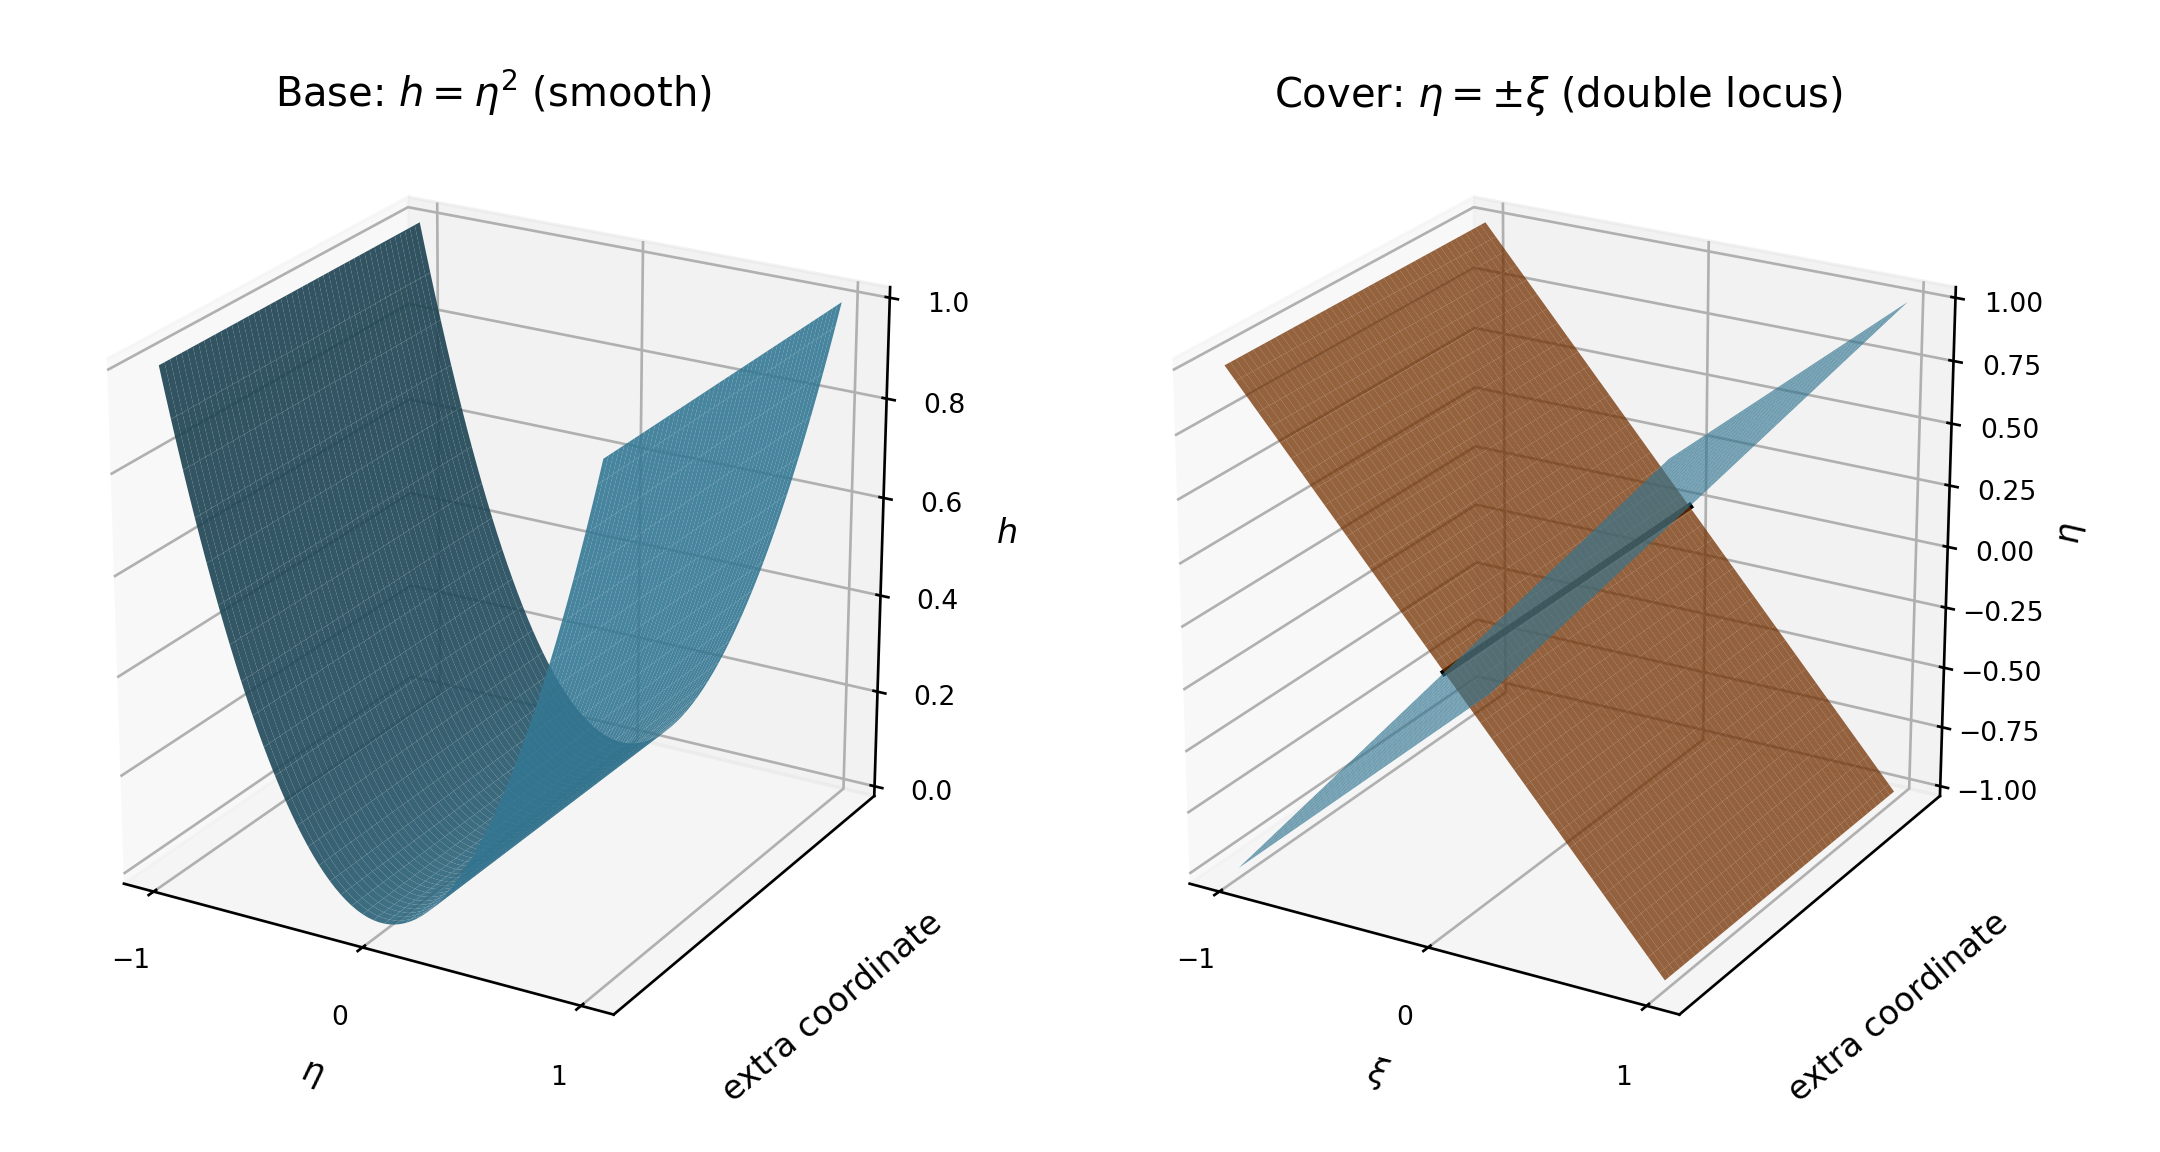
\includegraphics[width=0.94\linewidth,height=0.48\textheight,keepaspectratio]{figures/fig_base_cover.png}
\caption{Local distinction at $\chi=1$. The base divisor $h=\eta^2$ is smooth. Its pullback under $h=\xi^2$ consists of the crossing branches $\eta=\pm\xi$. The diagram displays real slices of complex divisors; it is a schematic, not a rendering of the full compactification.}
\label{fig:basecover}
\end{figure}

\subsection{Primary passages used for scope corrections}
The principal comparisons are reproducible from the following sources, with their original qualifications retained.
\begin{itemize}[leftmargin=1.4em,itemsep=2pt]
\item \cite{Sen11positivity}, introduction, pp.~3--5 and Eq.~(3.9): assumptions about hair and other index contributions, and the linear charge cone.
\item \cite{CD19}, Sections~4.1--4.2: known negative full indices in toroidal orbifolds; \cite{CD21}, Sections~4--5: proposed hair factors, finite positive horizon-index tests, and remaining mode-identification questions.
\item \cite{Sen02field}, Eqs.~(19)--(25): the pressureless Hamiltonian equations and the static solution with arbitrary density. The homogeneous decay assumption is stated in its abstract.
\item \cite{Sen97orientifold}, abstract, weak-coupling expansion and auxiliary double cover: the reduction is formal and singular auxiliary spaces are explicitly discussed. The D7 cover singularities are developed in \cite{CDE09}; global weak-coupling obstructions and the $I_0^*$ exception are in \cite{HLS18}.
\item \cite{Sen05stretching}, abstract and Gauss--Bonnet calculation: the higher-dimensional coefficient mismatch is reported by Sen, rather than discovered here.
\item \cite{Sen23localisation}: domain, ultraviolet and flat-direction issues are raised by Sen himself; they are not new unacknowledged objections.
\item \cite{FKS18}, Theorem~1.2 and Section~6, state the general coprime case using the announced metric compactification; \cite{KottkeRochon24}, Theorem~A: magnetic charge three is covered under the stated QFB-metric hypothesis. \cite{KrishnaSahoo23} separates proved one-loop universality from conjectural higher quantum extensions. \cite{KKMSS26} labels its beyond-Newtonian extension a conjecture.
\end{itemize}
This register is not evidence that every reference or every later citing paper has been independently checked. The bibliography supplies further context; new objections require their own exact source and hypothesis check.

\section{Two limits of perturbative reasoning}\label{app:perturbative}

\subsection{An exact leading-soft model}
Assume independent soft emissions with intensity $b\,d\omega/\omega$, $b\ge0$, an infrared cutoff $\lambda$, detector resolution $E$ and hard scale $\Lambda$, with $0<\lambda<E<\Lambda$. Assume also the virtual factor $\exp[-b\ln(\Lambda/\lambda)]$. Summing any number of unobserved emissions below $E$ gives
\begin{align}
P_\lambda&=e^{-b\ln(\Lambda/\lambda)}\sum_{n=0}^{\infty}
\frac{[b\ln(E/\lambda)]^n}{n!}\nonumber\\
&=e^{-b\ln(\Lambda/\lambda)+b\ln(E/\lambda)}
=e^{-b\ln(\Lambda/E)}.
\end{align}
The series is absolutely convergent and the last expression is independent of $\lambda$. This is a self-contained cancellation in the independent-emission model. It assumes soft factorisation and the virtual factor; it does not prove either for every string-field-theory diagram, include subleading emissions, or construct the general four-dimensional observable. The missing physical and analytic steps must not be concealed by the elementary exponential identity. The finite-exponent cancellation is separately checked in Lean.

\subsection{Formal unitarity does not determine a completion}
\begin{proposition}
There exist two smooth scalar amplitudes with the same Taylor series at zero coupling such that one is unitary and the other is not for every positive coupling.
\end{proposition}
\begin{proof}
Take $S_0(g)=1$ and $S_1(g)=1+f(g)$, where $f(0)=0$ and $f(g)=e^{-1/g^2}$ for $g\ne0$. For every integer $N\ge0$, choose an integer $m$ with $2m>N$. Since $e^t\ge t^m/m!$ for $t>0$,
\[
0\le |g|^{-N}f(g)\le m!|g|^{2m-N}\longrightarrow0.
\]
Each derivative of $f$ away from zero is a finite linear combination of powers of $g^{-1}$ times $f(g)$. Induction using the displayed bound extends every derivative continuously to zero with value zero. Thus both amplitudes have the same Taylor series, the constant $1$. It satisfies the formal scalar unitarity identity to every order, whereas $S_1(g)>1$ gives $|S_1(g)|^2>1$ for $g>0$.
\end{proof}
This is a counterexample to a general inference from a perturbative series to an exact completion, not a counterexample to Sen's perturbative theorem. The flat-function smoothness argument is proved here in ordinary analysis and is not part of the finite Lean certificate. A nonperturbative completion needs additional input such as a summation prescription, analytic class, boundary conditions or an independently constructed theory.

\section{A finite-energy infrared limit in an explicit soft model}\label{app:infraredlimit}

The leading-soft cancellation of Appendix~\ref{app:perturbative} can be strengthened to a construction allowing infinitely many unresolved quanta and a total-energy observable. The theorem below is a statement about an explicitly defined positive emission model. Its relation to a string amplitude requires additional factorisation estimates, stated afterwards. It is not a claimed solution of the full four-dimensional string-field-theory problem.

\begin{theorem}[finite-energy limit and quantitative cutoff removal]\label{thm:softmeasure}
Fix $b\ge0$ and $0<E<\Lambda$. For $0<\lambda<E$, let $N_\lambda$ be a Poisson random measure on $[\lambda,E]$ with intensity $b\,d\omega/\omega$, coupled by restriction of one measure on $(0,E]$. Put $S_\lambda=\int_{[\lambda,E]}\omega N(d\omega)$. There is a finite nonnegative random variable $S$ such that $S_\lambda\uparrow S$ almost surely and in $L^1$, and
\begin{align}
\mathbb E S&=bE,&\mathbb E|S-S_\lambda|&=b\lambda,\\
\mathbb E e^{-tS}&=\exp\left[b\int_0^E\frac{e^{-t\omega}-1}{\omega}\,d\omega\right]\quad(t\ge0).
\end{align}
For a bounded Lipschitz function $F:[0,\infty)\to\RR$, with Lipschitz constant $L_F$, define the inclusive model functional
\begin{align}
\mathcal I_\lambda(F)={}&e^{-b\ln(\Lambda/\lambda)}
\sum_{n=0}^{\infty}\frac{b^n}{n!}
\int_{[\lambda,E]^n}F\left(\sum_{j=1}^n\omega_j\right)
\prod_{j=1}^n\frac{d\omega_j}{\omega_j}.
\end{align}
Then
\begin{align}
\mathcal I_0(F)&=(E/\Lambda)^b\mathbb EF(S),\\
|\mathcal I_\lambda(F)-\mathcal I_0(F)|
&\le(E/\Lambda)^b L_F b\lambda.
\end{align}
If $b>0$, the total number of emitted quanta is infinite almost surely, although $S$ is finite, and the law of $S$ has no atoms. Consequently the cutoff also has a limit for each total-energy veto $F(s)=\mathbf1_{s\le\delta}$.
\end{theorem}

\begin{proof}
Partition $(0,E]$ into dyadic bands $J_k=(E2^{-k-1},E2^{-k}]$, $k\ge0$. On each band take an independent Poisson number with mean $b\ln2$, and conditional on that number take independent energies with density $1/(\omega\ln2)$ on the band. This constructs the measure on the product probability space without assuming a finite total particle number. The expectation of the energy in $J_k$ is $b|J_k|$, so the sum of the expectations is $bE$. The nonnegative total energy is therefore finite almost surely. Monotone convergence gives the almost-sure limit and
\[
\mathbb E(S-S_\lambda)=\int_0^\lambda\omega\,b\frac{d\omega}{\omega}=b\lambda.
\]

For a finite cutoff, the elementary generating function of a Poisson distribution yields
\[
\mathbb E e^{-tS_\lambda}=\exp\left[b\int_\lambda^E\frac{e^{-t\omega}-1}{\omega}\,d\omega\right].
\]
The bound $|e^{-t\omega}-1|\le t\omega$ makes the exponent integrable at zero. Dominated convergence proves the Laplace formula for $S$. Writing the Poisson expectation of $F(S_\lambda)$ as its absolutely convergent sum over particle numbers gives exactly
\[
\mathcal I_\lambda(F)=(E/\Lambda)^b\mathbb EF(S_\lambda).
\]
The Lipschitz estimate follows from the common coupling and the preceding $L^1$ identity.

If $b>0$, the count on $(\lambda,E]$ has Poisson mean $b\ln(E/\lambda)\to\infty$. For every fixed integer $K$, its probability of being at most $K$ tends to zero. Hence the total count is infinite almost surely. To prove absence of atoms, split at $a\in(0,E)$. The sum of energies in $[a,E]$, conditional on at least one emission, has a continuous distribution, since each energy has a density and convolutions retain that property. It is independent of the energies below $a$. Thus for every $x$,
\[
\mathbb P(S=x)\le\mathbb P(N([a,E])=0)=(a/E)^b.
\]
Let $a\downarrow0$. Finally $S_\lambda\to S$ almost surely, and the indicator of a fixed total-energy threshold is continuous away from an event of probability zero. Bounded convergence proves the final assertion. For $b=0$ the measure is concentrated at $S=0$ and the conclusion is immediate directly.
\end{proof}

This theorem treats total unresolved energy, not just a bound on each individual quantum. It also explains why a finite-energy limit need not be a finite-particle Fock vector. It constructs an energy distribution, not the angular momentum, memory algebra or gauge constraints of a gravitational quantum state.

\begin{proposition}[an explicit transfer criterion]
Let $\Sigma_\lambda(F)$ be a proposed regulated string observable. Suppose, for each observable in a specified class,
\[
\Sigma_\lambda(F)=H\mathcal I_\lambda(F)+R_\lambda(F),
\]
where $H$ is finite and independent of $\lambda$, and $R_\lambda(F)\to R_0(F)$ is separately proved. Then $\Sigma_\lambda(F)$ has a finite limit, with
\[
\Sigma_0(F)=H\mathcal I_0(F)+R_0(F).
\]
For Lipschitz $F$, its error is at most $|H|(E/\Lambda)^bL_Fb\lambda+|R_\lambda(F)-R_0(F)|$.
\end{proposition}
\begin{proof}
Subtract the two expressions and apply Theorem~\ref{thm:softmeasure} and the triangle inequality. The convergence assumption on the remainder is essential; the proposition does not establish it.
\end{proof}

\paragraph*{The remaining string-theory problem.} Weinberg's treatment \cite{Weinberg65} establishes the familiar gravitational soft cancellations in its stated setting. More recent algebraic scattering constructions \cite{PSW22,PS24} explicitly address the state-space problem. They do not justify silently replacing a constructed string-field evolution by an assumed automorphism. For the full string problem one must supply a specified stable compactification and observable, a common regulator compatible with the gauge identities, factorisation over all relevant degeneration regions, the corresponding virtual factors and measure, and control of collinear regions and overlapping limits. In the transfer proposition these obligations reside in the existence of $H$ and the convergence of $R_\lambda$. No proof of those obligations for every four-dimensional superstring background is supplied here. The Poisson construction and the scalar exponential identity are not Lean-formalised as probability theory in this release.

\section{A uniform single-soft estimate and the overlapping-limit obstruction}\label{app:softremainder}

This appendix makes one part of the transfer problem quantitative. The tree soft theorem is an established result of Sen \cite{Sen17tree}; the estimate below is a consequence on compact sets of massive hard kinematics, not a replacement for that theorem or a new proof of the complete four-dimensional infrared problem. We then give an exact example explaining why the same argument does not establish the required loop remainder.

\subsection{Kinematics and the tree pole decomposition}

Use signature $(+---)$ and write a future null soft momentum as $q=\omega n$, where $n=(1,\widehat n)$, $|\widehat n|=1$. The hard momenta $p_i$ are future timelike; incoming and outgoing legs have signs $\eta_i=-1$ and $+1$, respectively. At the limiting hard configuration, $\sum_i\eta_i p_i=0$. In the convention with linear coupling $-(\kappa/2)h_{\mu\nu}T^{\mu\nu}$, the leading coefficient for one physical graviton polarisation is
\begin{equation}\label{eq:softa}
 a(n)=\frac{\kappa}{2}\mathcal M_N
       \sum_i\eta_i\frac{\epsilon_{\mu\nu}(n)p_i^\mu p_i^\nu}{p_i\cdot n}.
\end{equation}
Here $\mathcal M_N$ is the stripped hard amplitude. A smooth on-shell recoil prescription is fixed when imposing momentum conservation at nonzero $q$. Its changes at order $\omega$ belong in the remainder. Formula~\eqref{eq:softa} is unchanged by $\epsilon_{\mu\nu}\mapsto\epsilon_{\mu\nu}+n_\mu\xi_\nu+\xi_\mu n_\nu$, since the change is $\kappa\mathcal M_N\xi\cdot\sum_i\eta_i p_i=0$.

Choose a compact set of nonsingular hard configurations, away from additional hard-channel poles and thresholds, and restrict to a recoil prescription defined on a neighbourhood of it. Since each hard leg is massive,
\begin{equation}\label{eq:massivegap}
 p_i\cdot n\ge p_i^0-|\boldsymbol p_i|
 =\frac{m_i^2}{p_i^0+|\boldsymbol p_i|}>0.
\end{equation}
After decreasing the upper soft energy $E$ if necessary, the same lower bound with a smaller positive constant holds uniformly along the recoil family. A physical helicity basis can be chosen in finitely many angular charts; the bounds below concern its invariant norms and do not require a globally smooth polarisation vector on the sphere.

In the tree sectors covered by \cite{Sen17tree}, use the usual meromorphic tree amplitude and its external-leg pole factorisation. On the selected compact neighbourhood it has the form
\begin{equation}\label{eq:poleform}
 \mathcal M_{N+1}(\omega,n)=\frac{1}{\omega}\sum_i f_i(\omega,n)+h(\omega,n),
 \qquad \sum_i f_i(0,n)=a(n),
\end{equation}
where the $f_i$ are continuously differentiable in $\omega$ and $h$ is bounded, uniformly in the hard configurations and the angular charts. These are tree analytic inputs, not assumptions about a loop amplitude. One obtains the $f_i$ by absorbing the nonzero factor $2\eta_i p_i(\omega,n)\cdot n$ into the numerator of each external-leg propagator. Other channels are regular by the choice of neighbourhood. The amplitude may contain infinitely many string poles elsewhere; the statement uses only local regularity away from those poles, rather than a truncation of the string spectrum.

\begin{proposition}[uniform tree remainder]\label{prop:treeremainder}
Let $H=\sup|h|$, $D_i=\sup|\partial_\omega f_i|$, and $C=H+\sum_iD_i$ on the neighbourhood just specified. Then
\begin{equation}\label{eq:treeR}
 \mathcal M_{N+1}(\omega,n)=\frac{a(n)}{\omega}+r(\omega,n),
 \qquad |r(\omega,n)|\le C\quad(0<\omega\le E).
\end{equation}
\end{proposition}
\begin{proof}
Subtract the coefficient at $\omega=0$ in \eqref{eq:poleform}. The fundamental theorem of calculus gives
\[
 r(\omega,n)=h(\omega,n)
       +\sum_i\int_0^1\partial_\omega f_i(t\omega,n)\,dt.
\]
The stated bound follows by the triangle inequality. All suprema are finite by the regularity and compactness hypotheses. The lower bound \eqref{eq:massivegap} is what makes the estimate uniform in angle for this argument. It supplies no such constant for a massless hard leg.
\end{proof}

\subsection{An explicit bound after the real-emission subtraction}

Let $\Omega$ be the angular and physical-polarisation space, with finite measure $\mu(\Omega)$; for both helicities integrated over the full sphere, $\mu(\Omega)=8\pi$. Put $A=\sup_\Omega|a|$. The one-particle phase-space convention is
\[
 d\Phi_q=\frac{\omega\,d\omega\,d\mu(n)}{2(2\pi)^3}.
\]
Let a real measurement function satisfy $|F(\omega,n)|\le B$ and $|F(\omega,n)-F(0,n)|\le L\omega$. Smooth recoil Jacobians and bounded hard-bin weights may be included in $F$ when these two estimates hold.

\begin{theorem}[integrable subtracted tree emission]\label{thm:realtail}
Under Proposition~\ref{prop:treeremainder}, define
\[
 T(\omega,n)=F(\omega,n)|\mathcal M_{N+1}(\omega,n)|^2
            -F(0,n)\frac{|a(n)|^2}{\omega^2}.
\]
The signed integral $\mathcal R_\lambda(F)=\int_{\lambda<\omega<E}T\,d\Phi_q$ has a limit as $\lambda\downarrow0$, and
\begin{equation}\label{eq:realtail}
 |\mathcal R_0(F)-\mathcal R_\lambda(F)|
 \le \frac{\mu(\Omega)}{2(2\pi)^3}
 \left[(LA^2+2BAC)\lambda+\frac{BC^2}{2}\lambda^2\right].
\end{equation}
\end{theorem}
\begin{proof}
The complex amplitude identity in \eqref{eq:treeR} gives
\[
 \left|\left|\frac a\omega+r\right|^2-\frac{|a|^2}{\omega^2}\right|
 \le\frac{2|a||r|}{\omega}+|r|^2.
\]
Separate $T$ into $(F-F(0,n))|a|^2/\omega^2$ and $F$ times the difference of the two squared amplitudes. Consequently
\[
 |T(\omega,n)|\le \frac{LA^2+2BAC}{\omega}+BC^2.
\]
Multiplication by the phase-space factor $\omega$ leaves an integrable bound at zero. Integrating it over $(0,\lambda)$ proves absolute convergence and \eqref{eq:realtail}.
\end{proof}

This proves cutoff removal for the \emph{subtracted single-real-emission tree sector}. It neither assigns a finite value to its unsubtracted logarithmic term nor supplies the corresponding virtual contribution. Those are separate ingredients in an inclusive observable.

The lower bound \eqref{eq:massivegap} applies to a real on-shell null $q$, not to an arbitrary virtual loop momentum. For example $p=(m,0,0,0)$ and $k=(0,\boldsymbol k)$ give $p\cdot k=0$ even when $\boldsymbol k\ne0$. Hence there is no estimate $|p\cdot k|\ge c\|k\|$ on the complete real loop domain merely because $p$ is massive. A virtual estimate must handle the pole prescription, contour and cancellations; it cannot be obtained by copying the real-emission angular bound.

\subsection{Logarithmic remainders: a sufficient quantitative bound}

A bounded tree remainder must not be assumed unchanged at four-dimensional loop level. Logarithmic soft terms are known \cite{SahooSen19}. Their presence alone does not prevent integration after the leading subtraction. For a nonnegative integer $m$, define
\begin{align}
 h_m(\omega)&=(1+\ln(E/\omega))^m,\\
 P_m(x)&=\sum_{j=0}^m\binom mj j!x^{m-j},\\
 Q_k(x)&=\sum_{j=0}^k\binom kj\frac{j!}{2^j}x^{k-j}.
\end{align}
For $0<\lambda\le E$ and $x=1+\ln(E/\lambda)$, direct integration gives
\begin{align}\label{eq:logmoments}
 \int_0^\lambda h_m(\omega)\,d\omega&=\lambda P_m(x),\\
 \int_0^\lambda\omega h_m(\omega)^2\,d\omega
 &=\frac{\lambda^2}{2}Q_{2m}(x).
\end{align}
Indeed put $\omega=\lambda e^{-u}$, expand $(x+u)^m$, and use $\int_0^\infty e^{-cu}u^jdu=j!/c^{j+1}$, proved by $j$ integrations by parts. The exponential decay makes each boundary term vanish.

\begin{proposition}[logarithmic extension]\label{prop:logremainder}
If a specified amplitude has the decomposition \eqref{eq:treeR} with the weaker bound $|r(\omega,n)|\le Ch_m(\omega)$, the same subtraction is absolutely integrable and its tail is at most
\begin{equation}\label{eq:logtail}
 \frac{\mu(\Omega)}{2(2\pi)^3}
 \left[LA^2\lambda+2BAC\lambda P_m(x)
       +\frac{BC^2\lambda^2}{2}Q_{2m}(x)\right].
\end{equation}
If a regulator-dependent family $r_\lambda$ has this bound with the \emph{same} $C,m$ and converges pointwise to $r_0$, its subtracted integrals converge by dominated convergence. If in addition $|r_\lambda-r_0|\le\varepsilon(\lambda)h_m$ for $\omega\ge\lambda$, their difference is bounded by the tail \eqref{eq:logtail} plus
\begin{equation}\label{eq:regmodulus}
 \frac{\mu(\Omega)}{2(2\pi)^3}\varepsilon(\lambda)
 \left[2BA E P_m(1)+BC E^2Q_{2m}(1)\right].
\end{equation}
\end{proposition}
\begin{proof}
Repeat the proof of Theorem~\ref{thm:realtail}, replacing $C$ by $Ch_m(\omega)$, and then use \eqref{eq:logmoments}. These moments give a regulator-independent integrable majorant when $C,m$ are uniform. For the quantitative last assertion,
\[
 \big||a/\omega+r_\lambda|^2-|a/\omega+r_0|^2\big|
 \le\frac{2A\varepsilon(\lambda)h_m}{\omega}
       +2C\varepsilon(\lambda)h_m^2.
\]
Integrate the right side with the measurement bound $B$ and phase space, extending its domain to $(0,E)$. This proves \eqref{eq:regmodulus}.
\end{proof}

The proposition does not assert that the remainders of every string loop amplitude satisfy its uniform hypothesis. Bounds whose constant diverges with the virtual infrared regulator do not meet it.

\subsection{Why separate soft limits do not control a corner}

\begin{proposition}[an overlapping-limit obstruction]\label{prop:softcorner}
For every fixed $x>0$, the integral $\int_0^E(x+y)^{-2}\,dy$ is finite, and the analogous statement holds with $x$ and $y$ exchanged. Nevertheless,
\begin{equation}\label{eq:corner}
 \int_\lambda^E\int_\lambda^E\frac{dx\,dy}{(x+y)^2}
 =\ln\frac{(E+\lambda)^2}{4E\lambda}
 \longrightarrow+\infty.
\end{equation}
\end{proposition}
\begin{proof}
The first assertion follows from the antiderivative $-1/(x+y)$. Integrating first in $x$ gives $1/(\lambda+y)-1/(E+y)$. Integrating in $y$ yields \eqref{eq:corner}. In coordinates $r=x+y$, $t=x/(x+y)$, the Jacobian has absolute value $r$, so the density becomes $dr\,dt/r$. Resolving the corner by this change of variables exposes a logarithmic radial divergence; it does not remove it.
\end{proof}

This is an analytic counterexample to an inference from separate integrability to joint integrability. It is not asserted to be an actual string diagram or a counterexample to a gravitational Ward identity. It shows why a proof about one soft external momentum cannot replace an estimate at every overlapping degeneration.

For clarity, the useful estimate after such a resolution can also be stated exactly. Suppose one \emph{subtracted} sector of an integral is represented by variables $u_j\in(0,1]$, an angular variable $\theta$, and density
\[
 G(u,\theta)\prod_{j=1}^s\frac{du_j}{u_j}\,d\nu(\theta).
\]
If there are $\delta_j>0$ and an integrable $C(\theta)\ge0$ with
\begin{equation}\label{eq:sectorbound}
 |G(u,\theta)|\le C(\theta)\prod_j u_j^{\delta_j},
\end{equation}
then its absolute integral is at most $\|C\|_1\prod_j\delta_j^{-1}$. Removing the region where any $u_j<t$ changes the integral by at most
\begin{equation}\label{eq:sectortail}
 \|C\|_1\left(\prod_j\delta_j^{-1}\right)\sum_jt^{\delta_j}.
\end{equation}
This follows from Tonelli's theorem, $\int_0^t u^{\delta-1}du=t^\delta/\delta$, and a union bound on the removed regions. The argument proves a sufficient estimate once the sector representation and its bound are established. It does not establish \eqref{eq:sectorbound} for the string integrand or identify the physical regulator with this box cutoff.

\subsection{A useful power count for the pure-graviton soft sector}

There is also an all-graph homogeneous estimate worth separating from a full convergence theorem. Consider soft graviton propagators connecting massive eikonal lines. Suppose there are $I$ soft propagators, $V$ internal soft interaction vertices of valences $d_v\ge3$, and $E_a$ attachments to the eikonal lines. Take each interaction to have at least two soft derivatives. Exclude vacuum components and tadpoles; absorb two-point kinetic insertions into the propagator. Assume the $V$ internal momentum-conservation constraints are independent, so the number of independent soft loop momenta is $\ell=I-V$. Incidence counting gives $E_a=2I-\sum_vd_v$.

Under a uniform rescaling of all these loop momenta by $r$, the loop measures, soft propagators, eikonal denominators and vertex numerators have total degree at least
\begin{equation}\label{eq:gravdegree}
 \gamma=4\ell-2I-E_a+2V
        =\sum_v(d_v-2).
\end{equation}
Thus $V>0$ implies $\gamma\ge V>0$, whereas $V=0$ gives the marginal degree zero of independent exchanges. The equality follows by substitution of the two counting identities; the inequality uses $d_v\ge3$. If the remaining angular factors are bounded, a radial integral has density bounded by a constant times $r^{\gamma-1}dr$ and converges for $\gamma>0$.

This is consistent with the established gravitational infrared analysis \cite{ASS11}. It explains the distinguished role of independent eikonal exchanges. It is not a bound on every partial rescaling: if some momenta stay fixed, a vertex need not supply two powers of the momenta being scaled. Nor does the count bound angular pinch surfaces or other massless species. To use it in \eqref{eq:sectorbound}, every nested and overlapping scaling region must be controlled after the relevant Ward-identity cancellations. A favourable homogeneous degree for the whole graph does not prove this last assertion.

\subsection{What remains for the full string-field-theory observable}

Gravitational soft factorisation and cancellation results extend well beyond a single tree diagram \cite{Weinberg65,ASS11}. Those results must retain their scattering assumptions and the cancellations between complete sets of diagrams. They do not identify an arbitrary positive Poisson model with a complete compactified string theory containing its other massless fields.

To apply the transfer proposition of Appendix~\ref{app:infraredlimit}, one still needs a specified background, external states and infrared-safe measurement; the common real and virtual regulator; and a subtraction construction compatible with the gauge identities. At each fixed perturbative order that construction must control every simultaneous soft, collinear and degeneration region, the relevant string-state sums, and the remaining hard coefficient. A sufficient route is a uniform integrable bound after all required cancellations, such as \eqref{eq:sectorbound}, on the appropriate contours or cut phase spaces, with control of regulator removal. A rigorously controlled distributional limit could provide another route. Neither route is supplied for the complete observable here. An ordinary nonperturbative S-matrix would require further construction, beyond finiteness at each order.

The tree estimate \eqref{eq:realtail}, the logarithmic integration formulas and the corner calculation are established here. A factorisation theorem and convergent remainder for the complete four-dimensional string-field observable have not been proved. The finite algebraic certificates accompanying this appendix do not formalise the soft theorem, the phase-space integrals or the full string amplitude.

\section{Proofs for the Sen limit and the small black holes}\label{app:closures}

This appendix proves the results of Sections~\ref{ssec:normalform} and~\ref{ssec:small}. Every step is written out; the only external inputs are the adjunction formula, the standard facts on double covers of surfaces recalled in the proof of Corollary~\ref{cor:k3cover}, and the Euler numbers of the Kodaira fibres $I_1$ and $II$.

\subsection{The weak coupling limit}

Throughout, $B$ is a normal projective variety, $L$ a line bundle on $B$, and $v$ the $\eps$-adic valuation: for a series $s=\sum_is_i\eps^i$ with coefficients $s_i\in H^0(B,L^k)$, $v(s)=\min\{i:s_i\ne0\}$. Since $B$ is irreducible, the ring $\bigoplus_kH^0(B,L^k)$ has no zero divisors, so $v(st)=v(s)+v(t)$ and $v(s+t)\ge\min(v(s),v(t))$, with equality when $v(s)\ne v(t)$.

\begin{proof}[Proof of Theorem~\ref{thm:normalform}]
\emph{Step 1.} Neither $f$ nor $g$ vanishes identically: if $f\equiv0$ then $j\equiv0$, and if $g\equiv0$ then $j\equiv1728$. Put $a=v(f)$, $b=v(g)$, $d=v(\Delta)$, so that $v(j)=3a-d$.

\emph{Step 2.} If $3a<2b$, the term $4f^3$ has the smaller valuation, $d=3a$ and $v(j)=0$. If $3a>2b$, then $d=2b$ and $v(j)=3a-2b>0$. Neither is weakly coupled, so $3a=2b$; hence $a=2c$, $b=3c$ for an integer $c\ge0$, and $d>3a$ because $v(j)<0$.

\emph{Step 3.} If $c$ is odd, the base change $\eps=t^2$ doubles every valuation and makes $c$ even. With $c=2r$, the rescaling $(f,g)\mapsto(t^{-4r}f,t^{-6r}g)$ gives $v(f)=v(g)=0$ and $v(\Delta)>0$. The coefficients are still sections of $L^4$ and $L^6$, and no negative powers of $t$ occur because $a$ and $b$ were the least exponents. The order of the base change so far is $k_1\in\{1,2\}$.

\emph{Step 4.} Let $f_0,g_0$ be the coefficients of $t^0$. They are nonzero, and the coefficient of $t^0$ in $\Delta$ gives $4f_0^3+27g_0^2=0$. The quotient $h=3g_0/(2f_0)$ is a rational section of $L^2$, and
\[
h^2=\frac{9g_0^2}{4f_0^2}=\frac{9}{4f_0^2}\cdot\Big(-\frac{4f_0^3}{27}\Big)=-\frac{f_0}{3},\qquad h^3=h\cdot h^2=-\frac{g_0}{2}.
\]
In a trivialisation of $L$ near a point of $B$, $h$ is a rational function whose square is regular, so it is a root of the monic polynomial $X^2-h^2$ over the local ring. The local ring of a normal variety is integrally closed, so $h$ is regular. Thus $h\in H^0(B,L^2)$, $h\ne0$, $f_0=-3h^2$ and $g_0=-2h^3$, which also proves part~(iii).

\emph{Step 5.} Write $f=-3h^2+tF$ and $g=-2h^3+tG$ with $F\in H^0(L^4)[[t]]$ and $G\in H^0(L^6)[[t]]$. Expanding,
\[
\Delta=4(-3h^2+tF)^3+27(-2h^3+tG)^2=108\,t\,h^3\big(hF_0-G_0\big)+O(t^2),
\]
since $4\cdot3\cdot9h^4=108h^4$ and $27\cdot2\cdot2h^3=108h^3$. If $G_0=hF_0$, then $G-hF=t\Psi$ for a series $\Psi$, and $\eta_t=F$, $\chi_t=-12\Psi$ give
\[
-2h^3+t\,h\,\eta_t-\tfrac1{12}t^2\chi_t=-2h^3+t\,hF+t^2\Psi=-2h^3+tG=g,
\]
which is \eqref{eq:normalform} with $k=k_1$. If $G_0\ne hF_0$, make the base change $t=s^2$ and put $\eta_s=sF(s^2)$, $\chi_s=-12\big(G(s^2)-hF(s^2)\big)$. Then $-3h^2+s\eta_s=-3h^2+s^2F(s^2)=f$ and
\[
-2h^3+s\,h\,\eta_s-\tfrac1{12}s^2\chi_s=-2h^3+s^2hF(s^2)+s^2\big(G(s^2)-hF(s^2)\big)=-2h^3+s^2G(s^2)=g,
\]
which is \eqref{eq:normalform} in the parameter $s$, with $k=2k_1\in\{2,4\}$. This proves part~(i).

\emph{Part (ii).} If $h\ne0$, then $f_0=-3h^2\ne0$ and $v(f)=0$. The identity of Theorem~\ref{thm:senlimitk3} is a polynomial identity in $t,h,\eta,\chi$, so it holds with $\eta_t,\chi_t$ in place of $\eta,\chi$: $\Delta$ is divisible by $t^2$. Hence $v(j)=-v(\Delta)\le-2$.
\end{proof}

\begin{proof}[Proof of Corollary~\ref{cor:existence}]
A weakly coupled degeneration produces $h\in H^0(L^2)\setminus0$ by Theorem~\ref{thm:normalform}(i). Conversely, for $h\ne0$ take $\eta=h^2$ and $\chi=0$. Theorem~\ref{thm:senlimitk3} gives $\Delta=-9t^2h^6+4t^3h^6=h^6t^2(4t-9)\not\equiv0$, so the family is weakly coupled by Theorem~\ref{thm:normalform}(ii). Since $f=(t-3)h^2$, $4f^3=4(t-3)^3h^6$, and the factor $h^6$ cancels in $j=1728\cdot4f^3/\Delta$.
\end{proof}

\begin{proof}[Proof of Proposition~\ref{prop:rigidcurves}]
(i) By adjunction $K_B\cdot C+C^2=2g(C)-2=-2$, so $L\cdot C=-K_B\cdot C=2-n$. Let $s\in H^0(L^k)$ vanish to order exactly $a$ on $C$, and write $s=\sigma^as'$ with $\sigma$ a section of $\mathcal O(C)$ defining $C$. Then $s'$ is a section of $L^k(-aC)$ that does not vanish identically on $C\cong\PP^1$, so its restriction is a nonzero section of a line bundle of degree $(kL-aC)\cdot C=k(2-n)+an$. This degree is nonnegative, so $a\ge k(n-2)/n$. For $n\ge5$, $4(n-2)/n\ge12/5$ and $6(n-2)/n\ge18/5$, so $\operatorname{ord}_Cf\ge3$ and $\operatorname{ord}_Cg\ge4$.

(ii) Let $a=\operatorname{ord}_Cf\ge3$ and $b=\operatorname{ord}_Cg\ge4$. If $3a=2b$, then $a$ is even, so $a\ge4$ and $b=3a/2\ge6$, and the model is not minimal along $C$. If $3a<2b$, then $\Delta=\sigma^{3a}\Delta'$ with $\Delta'\equiv4f'^3\pmod\sigma$ where $f=\sigma^af'$, and $j=1728\cdot4f'^3/\Delta'$ equals $1728$ at the generic point of $C$. If $3a>2b$, then $\Delta=\sigma^{2b}\Delta'$ with $\Delta'\equiv27g'^2\pmod\sigma$ and $j=1728\cdot4\sigma^{3a-2b}f'^3/\Delta'$ vanishes on $C$.

(iii) In the normal form $h$ is a section of $L^2$, so by part~(i) with $k=2$ it vanishes on $C$ to order at least $\lceil2(n-2)/n\rceil$, which is $2$ for $n\ge5$ and $1$ for $n=3,4$. Base change and rescaling do not change $h$ (Step~4 above).
\end{proof}

\begin{proof}[Proof of Corollary~\ref{cor:k3cover}]
We use the following facts on a double cover $\pi:X\to B$ of a smooth surface branched along a divisor $O\in|L^2|$, given by $\xi^2=h$ in the total space of $L$ \cite[Chapters~I and~III]{BHPV04}: $\pi_*\mathcal O_X=\mathcal O_B\oplus L^{-1}$; $X$ is normal if and only if $O$ is reduced; if $O$ is reduced with at most simple singularities, $X$ has at most rational double points; and the dualising sheaf is $\omega_X=\pi^*(K_B\otimes L)$.

(i) With $L=K_B^{-1}$, $\omega_X=\pi^*\mathcal O_B=\mathcal O_X$. Rational double points are canonical, so the minimal resolution $\widetilde X$ has trivial canonical bundle. For rational $B$, $h^1(\mathcal O_X)=h^1(\mathcal O_B)+h^1(K_B)=0+h^1(\mathcal O_B)=0$ by Serre duality, so $\widetilde X$ is a K3 surface.

(ii) On an Enriques surface $K_B\ne0$ and $2K_B=0$, so $L^2$, $L^4$ and $L^6$ are trivial and their sections are constants. Thus $h$ is a nonzero constant, $f$ and $g$ are series with constant coefficients, and $j$ does not depend on the point of $B$. The equation $\xi^2=h$ with $\xi$ a section of $K_B$ defines the unramified double cover attached to the two-torsion class $K_B$, which is the K3 surface covering $B$. The discriminant is a nonzero constant for $\eps\ne0$ small, so there is no seven-brane, and $O=\emptyset$.

(iii) We assume, as for $\PP^2$ and the del Pezzo surfaces of degree at least two, that $|{-K_B}|$ has no base points, so that $|{-kK_B}|$ has none for $k\ge1$. By Bertini's theorem a general $h$ defines a smooth curve $O$, and a general $\eta_0$ meets it transversally in $(-2K_B)\cdot(-4K_B)=8K_B^2$ points, at which a general $\chi_0$ does not vanish. The linear system of the curves $\eta_0^2=h\chi_0$, with $h$ fixed, has no base points: at a point with $h\ne0$ some member does not vanish, and at a point with $h=0$ the member $\eta_0^2$ does not vanish for a suitable $\eta_0$. By Bertini's theorem its general member $D_B$ is smooth. A point of $D_B\cap O$ has $h=0$ and hence $\eta_0=0$. Near such a point $(h,\eta_0)$ are local coordinates and $D_B$ is the graph $h=\eta_0^2/\chi_0$, which is tangent to $O=\{h=0\}$ with intersection multiplicity $2$; this accounts for $D_B\cdot O=16K_B^2=2\cdot8K_B^2$. On $X$, $(\xi,\eta_0)$ are local coordinates and $D_X=\{\eta_0^2=\xi^2\chi_0\}$ has the two branches $\eta_0=\pm\xi\sqrt{\chi_0}$, a node. Each branch, parametrised by $\xi$, maps to $D_B$, parametrised by $\eta_0=\pm\xi\sqrt{\chi_0}$, isomorphically. Away from $O$ the map $\pi$ is unramified. Hence the normalisation $\widetilde D$ of $D_X$ is an unramified double cover of $D_B$.

(iv) For a curve $\Gamma$ on $B$ of arithmetic genus $p_a$, $2p_a-2=\Gamma\cdot(\Gamma+K_B)$. For the smooth curves $O\in|{-2K_B}|$ and $D_B\in|{-8K_B}|$ this gives $\chi(O)=-(-2K_B)\cdot(-K_B)=-2K_B^2$ and $\chi(D_B)=-(-8K_B)\cdot(-7K_B)=-56K_B^2$, and an unramified double cover doubles the Euler characteristic, $\chi(\widetilde D)=-112K_B^2$. For general $f,g$ the discriminant $\Delta\in|{-12K_B}|$ has ordinary cusps at the $(-4K_B)\cdot(-6K_B)=24K_B^2$ points $f=g=0$, with fibres of type $II$ and Euler number $2$, and is smooth elsewhere, with fibres of type $I_1$ and Euler number $1$. Its arithmetic genus satisfies $2p_a-2=132K_B^2$; each cusp lowers the geometric genus by one and has one preimage in the normalisation, so $\chi(\Delta)=2-2(p_a-24K_B^2)=-84K_B^2$. The smooth fibres have Euler number $0$, so
\[
\chi(Y)=1\cdot\big(\chi(\Delta)-24K_B^2\big)+2\cdot24K_B^2=-108K_B^2+48K_B^2=-60K_B^2.
\]
Finally $4\chi(O)+\chi(\widetilde D)=-8K_B^2-112K_B^2=-120K_B^2=2\chi(Y)$. For $B=\PP^2$, $K_B^2=9$ and $\chi(Y)=-540$.
\end{proof}

\subsection{The small black holes}

\begin{proof}[Proof of Theorem~\ref{thm:twocharge}]
Write $P=2(u_T^2e_1^2+e_2^2u_T^{-2})$ and $F=v_1v_2^{n_D/2}\big[P/v_1^2+Q\big]=v_2^{n_D/2}v_1^{-1}\big(P-R\big)$, so that $f=Ku_SF$. The equations of the entropy function \cite[Section~3]{Prester06} are $\partial f/\partial u_S=\partial f/\partial u_T=\partial f/\partial v_1=\partial f/\partial v_2=0$ and $\partial f/\partial e_i=q_i$, and the entropy is $2\pi(e_1q_1+e_2q_2-f)$.

The equation for $u_S$ is $F=0$, that is $P=R$; in particular $f=0$ on a solution. The equation for $u_T$ is $\partial P/\partial u_T=0$, that is $u_T^2e_1^2=e_2^2u_T^{-2}$, so $u_T^2=e_2/e_1$ and $P=4e_1e_2$. The charges are
\[
q_1=Ku_Sv_2^{n_D/2}\frac{4u_T^2e_1}{v_1},\qquad q_2=Ku_Sv_2^{n_D/2}\frac{4e_2}{u_T^2v_1},
\]
so with $\kappa=Ku_Sv_2^{n_D/2}/v_1$ one has $e_1q_1=e_2q_2=4\kappa u_T^2e_1^2=\kappa P$ and $q_1q_2=16\kappa^2e_1e_2=4\kappa^2P$. Hence
\[
S_{\rm BH}=2\pi(e_1q_1+e_2q_2)=4\pi\kappa P=2\pi\sqrt{q_1q_2P}=4\pi\sqrt{nw\,P/\alpha'}.
\]
At fixed $u_S,u_T,e_i$ and on the locus $P=R$,
\[
\frac{\partial F}{\partial v_1}=-\frac{v_2^{n_D/2}}{v_1}\frac{\partial R}{\partial v_1},\qquad\frac{\partial F}{\partial v_2}=-\frac{v_2^{n_D/2}}{v_1}\frac{\partial R}{\partial v_2},
\]
because the derivatives of the prefactor multiply $P-R=0$. So a solution is a critical point of $R$ with $R=P=4e_1e_2>0$, and $S_{\rm BH}=4\pi\sqrt{nwR_*/\alpha'}$.

Conversely, given a critical point with $R_*>0$ and charges $n,w>0$, the equations $P=R_*$, $u_T^2=e_2/e_1$ and $q_1/q_2=e_2/e_1$ determine $e_1e_2=R_*/4$ and $e_2/e_1=n/w$, hence $e_1,e_2,u_T$, and then $q_1$ determines $u_S>0$. So the correspondence is a bijection. The statistical value requires $R_*=\alpha'$, that is $e_1e_2=\alpha'/4$.
\end{proof}

\begin{proof}[Proof of Corollary~\ref{cor:lovelock}]
With $Q=H-G/v_1$, $R=v_1G-v_1^2H$, so $\partial_{v_1}R=G-2v_1H$ and $\partial_{v_2}R=v_1(G'-v_1H')$. At a critical point $G=2v_1H$, and then $R=v_1^2H$; since $R>0$ and $v_1>0$, $H>0$ and $G>0$. Substituting $v_1=G/(2H)$, $R_*=G^2/(4H)=\Phi/4$, and
\[
G'-v_1H'=\frac{2G'H-GH'}{2H}=\frac{H^2\Phi'}{2GH},\qquad\Phi'=\frac{G\,(2G'H-GH')}{H^2},
\]
so $\partial_{v_2}R=0$ if and only if $\Phi'=0$. Conversely a critical point of $\Phi$ with $G,H>0$ gives $v_1=G/(2H)>0$ and a critical point of $R$ with $R_*=\Phi/4>0$. By Theorem~\ref{thm:twocharge}, $S_{\rm BH}=4\pi\sqrt{nw\Phi/4}=2\pi\sqrt{nw\Phi}$.
\end{proof}

\begin{proof}[Proof of Corollary~\ref{cor:gb}]
For $\lambda_1=1$, $\lambda_2=1/8$, \eqref{eq:GH} gives $G=2+a/(2y)$ and $H=(a/y)\big(1+b/(8y)\big)$, since $n_D(n_D-1)=a$ and $n_D(n_D-1)(n_D-2)(n_D-3)=ab$. Put $u=a/y$ and $\rho=b/(8a)$, so that $\Phi=(2+u/2)^2/\big(u(1+\rho u)\big)$. Both $G$ and $H$ are positive for $y>0$. The logarithmic derivative in $u$ vanishes when
\[
\frac{1}{2+u/2}=\frac1u+\frac{\rho}{1+\rho u}=\frac{1+2\rho u}{u(1+\rho u)},
\]
that is $2u(1+\rho u)=(4+u)(1+2\rho u)$, which reduces to $u(1-8\rho)=4$. Since $8\rho=b/a<1$, there is exactly one solution, $u=4a/(a-b)$, so $y=(a-b)/4$. There
\[
G=\frac{2(2a-b)}{a-b},\qquad H=\frac{4a}{a-b}\cdot\frac{2a-b}{2(a-b)},\qquad \Phi_*=\frac{G^2}{H}=\frac{2(2a-b)}{a}=4-\frac{2b}{a},
\]
and $v_1=G/(2H)=(a-b)/(2a)=2y/a$. By Corollary~\ref{cor:lovelock}, $S_{\rm BH}/(4\pi\sqrt{nw})=\sqrt{\Phi_*/4}=\sqrt{1-b/(2a)}$. Since $\Phi\to\infty$ as $u\to0$ and as $u\to\infty$, the critical point is the minimum. The ratio $b/a$ increases with $D\ge5$ and tends to $1$, which gives the limit $1/\sqrt2$. In \eqref{eq:sen320}, $a_D/a_4=\big\{(2/a)(8a-4b)\big\}^{1/2}/4=\sqrt{1-b/(2a)}$, independently of $C$.
\end{proof}

\begin{proof}[Proof of Theorem~\ref{thm:prester}]
(i) Shifting the index by one in $G$,
\[
G=2\lambda_1+\sum_{k\ge1}\frac{2(k+1)\lambda_{k+1}n_D!}{(n_D-2k)!}\,y^{-k},\qquad H=\sum_{k\ge1}\frac{\lambda_k\,n_D!}{(n_D-2k)!}\,y^{-k},
\]
both sums running over $1\le k\le\lfloor n_D/2\rfloor$. So $H=2(G-2\lambda_1)$ if and only if $\lambda_k=4(k+1)\lambda_{k+1}$ for these $k$, which holds for $\lambda_k=4^{1-k}/k!$.

(ii) With $H=2(G-2)$, $R=v_1G-2v_1^2(G-2)=4v_1^2+v_1G\,(1-2v_1)$. On $v_1=1/2$ this is $1$. Moreover $\partial_{v_2}R=v_1G'(1-2v_1)$, and $G'<0$ because every term of $G-2$ is a positive multiple of a negative power of $y$, and the term $k=1$ is present for $n_D\ge2$. So a critical point with $v_1>0$ has $v_1=1/2$. Then $\partial_{v_1}R=8v_1+G(1-4v_1)=4-G$ vanishes when $G=4$, equivalently $H=4$, and $R_*=1$. Theorem~\ref{thm:twocharge} gives $S_{\rm BH}=4\pi\sqrt{nw}$.

(iii) $H(y)=\sum_{k=1}^{\lfloor n_D/2\rfloor}c_ky^{-k}$ with every $c_k>0$, so $H$ decreases strictly from $+\infty$ to $0$ on $(0,\infty)$ and $H=4$ has exactly one positive root. Since $\lambda_mn_D!/(n_D-2m)!=4\,(n_D)_{2m}/(m!\,4^m)$ with $(N)_{j}=N(N-1)\cdots(N-j+1)$, and $(2m)!/m!=2^m(2m-1)!!$,
\[
\frac H4+1=\sum_{m\ge0}\frac{(n_D)_{2m}}{m!\,(4y)^m}=\sum_{m\ge0}\binom{n_D}{2m}(2m-1)!!\Big(\frac1{2y}\Big)^m=I_{n_D}\Big(\frac1{2y}\Big).
\]
A set of $m$ disjoint pairs in an $N$-element set is chosen in $\binom N{2m}(2m-1)!!$ ways, which is the stated count of involutions. With $\operatorname{He}_N(x)=\sum_m(-1)^m\binom N{2m}(2m-1)!!\,x^{N-2m}$ one has $i^{-N}\operatorname{He}_N(ix)=\sum_m\binom N{2m}(2m-1)!!\,x^{N-2m}=x^NI_N(x^{-2})$, and $x=\sqrt{2y}$ gives the Hermite form.

(iv) Put $N=n_D$ and $x=N^2/(4y)$, so that $I_N(1/(2y))=F_N(x)$ with
\[
F_N(x)=\sum_{m\le N/2}\frac{x^m}{m!}\prod_{j=0}^{2m-1}\Big(1-\frac jN\Big).
\]
For numbers $a_j\in[0,1]$ with sum $\sigma$, $1-\sigma\le\prod(1-a_j)\le1-\sigma+\sigma^2/2$. Here $\sigma=m(2m-1)/N$, so the product is $1-m(2m-1)/N+O(m^4/N^2)$ with an absolute constant. Since $\sum_m m(2m-1)x^m/m!=(2x^2+x)e^x$ and $\sum_m m^4x^m/m!$ is bounded on $[0,2]$, and since the terms with $m>N/2$ of these series and of $e^x$ are at most $\sum_{m>N/2}m^4 2^m/m!=O(N^{-2})$ for $x\in[0,2]$,
\[
F_N(x)=e^x\Big(1-\frac{2x^2+x}{N}\Big)+O(N^{-2})\quad\text{uniformly on }[0,2].
\]
$F_N$ is increasing, $F_N(0)=1$ and $F_N(2)\to e^2>2$, so the root $x_N$ of $F_N=2$ lies in $(0,2)$ for large $N$, and the derivative of the right-hand side is bounded away from $0$ near $\ln2$. Hence $x_N=\ln2+(2\ln^22+\ln2)/N+O(N^{-2})$, and
\[
y_D=\frac{N^2}{4x_N}=\frac{N^2}{4\ln2}\Big(1-\frac{2\ln2+1}{N}+O(N^{-2})\Big)=\frac{N^2}{4\ln2}-\frac{(2\ln2+1)N}{4\ln2}+O(1).\qedhere
\]
\end{proof}

\begin{proof}[Proof of Theorem~\ref{thm:rigidity}]
Write $p_k=4^{1-k}/k!$ and $N=n_D$.

(i) The coefficient $\lambda_m$ enters $H$ only if $N-2m\ge0$, and $N-2m=-2$ for $D=2m$ and $-1$ for $D=2m+1$. It enters $G$ through the term $2m\lambda_mN!/(N+2-2m)!\,y^{1-m}$, with $N+2-2m=0$ or $1$. Hence $G_\beta=G_1+(\beta-1)c\,y^{1-m}$ with $c>0$, and $H$ does not depend on $\beta$. All coefficients of $G_\beta$ and $H$ are positive, so both are positive on $(0,\infty)$. As $y\to\infty$, $G_\beta\to2$ and $H\to0^+$, so $\Phi_\beta\to\infty$. As $y\to0$, $G_\beta\sim\beta c\,y^{1-m}$ and $H\sim c'y^{1-m}$ with $c'>0$, the leading term of $H$ having index $m-1$ in both parities, so $\Phi_\beta\sim(\beta c)^2y^{1-m}/c'\to\infty$ since $m\ge2$. The minimum is attained.

(ii) By Theorem~\ref{thm:prester}(i), $H=2(G_1-2)$, so $\Phi_1-4=(G_1^2-8G_1+16)/H=(G_1-4)^2/H\ge0$ for all $y>0$. If $\beta>1$, then $G_\beta>G_1>0$ and $\Phi_\beta>\Phi_1\ge4$ everywhere, so every critical point has $\Phi_\beta>4$ and, by Corollary~\ref{cor:lovelock}, $S_{\rm BH}>4\pi\sqrt{nw}$.

(iii) If $0<\beta<1$, then at the root $y_D$ of Theorem~\ref{thm:prester}, $0<G_\beta(y_D)<G_1(y_D)=4$ and $\Phi_\beta(y_D)<16/4=4$. So the minimum of $\Phi_\beta$ is below $4$, and the solution there has $S_{\rm BH}<4\pi\sqrt{nw}$.

For the last statement, argue by induction on $m\ge2$ in $D=2m$, where $\lambda_1,\dots,\lambda_m$ are the only coefficients present. If $\lambda_k=p_k$ for $k<m$, write $\lambda_m=\beta p_m$ with $\beta>0$; parts~(ii) and~(iii) leave only $\beta=1$.
\end{proof}


\section*{Declarations}

\subsection*{Funding} None.

\subsection*{Conflict of interest} None.

\subsection*{Ethics statement} Not applicable: this work involves no human participants, animals or personal data.

\subsection*{Data availability} The program that computes the Fourier coefficients of Appendix~\ref{app:computation} and every table of this paper, the Lean~4 certificates of its finite statements, the scripts that check the explicit constants of Appendices~\ref{app:infraredlimit} and~\ref{app:softremainder}, the identities of Appendix~\ref{app:closures} and the identities and values used in the proofs of Theorems~\ref{thm:chlpositivity}, \ref{thm:chlunit} and~\ref{thm:chlunitodd}, the enumeration of orbits and the coefficients of Theorem~\ref{thm:chlbounded}, and the source of the paper are archived on Zenodo, \href{https://doi.org/\zenodoCodeID}{doi:\zenodoCodeID} \cite{Bha26}. The catalogue of Section~\ref{sec:catalogue} is kept in the ledger format of the engine Anaxia \cite{BLLM26}. The source register in Appendix~\ref{app:scopechecks} records the primary passages used for the scope corrections. The programs, the Lean certificates and parts of the text were prepared with the assistance of Claude Code (Anthropic); the authors checked every proof and every computation and take full responsibility for the paper.

\begingroup\sloppy\emergencystretch=5em\begin{thebibliography}{99}
\providecommand{\doilink}[1]{\href{https://doi.org/#1}{\nolinkurl{doi:#1}}}
\providecommand{\arxivlink}[1]{\href{https://arxiv.org/abs/#1}{\nolinkurl{arXiv:#1}}}
\bibitem{AGJST06} D. Astefanesei, K. Goldstein, R. P. Jena, A. Sen and S. P. Trivedi, \emph{Rotating attractors}, JHEP \textbf{10} (2006) 058, \doilink{10.1088/1126-6708/2006/10/058}, \arxivlink{hep-th/0606244}.
\bibitem{AKS06} P. C. Argyres, A. Kapustin and N. Seiberg, \emph{On $S$-duality for non-simply-laced gauge groups}, JHEP \textbf{06} (2006) 043, \doilink{10.1088/1126-6708/2006/06/043}, \arxivlink{hep-th/0603048}.
\bibitem{AtiyahHitchin88} M.~F. Atiyah and N.~J. Hitchin, \emph{The geometry and dynamics of magnetic monopoles}, Princeton University Press, Princeton (1988), \doilink{10.1515/9781400859306}.
\bibitem{Barnaby04} N. Barnaby, \emph{Caustic formation in tachyon effective field theories}, JHEP \textbf{07} (2004) 025, \doilink{10.1088/1126-6708/2004/07/025}, \arxivlink{hep-th/0406120}.
\bibitem{BBGMS10} N. Banerjee, S. Banerjee, R. K. Gupta, I. Mandal and A. Sen, \emph{Supersymmetry, Localization and Quantum Entropy Function}, JHEP \textbf{02} (2010) 091, \doilink{10.1007/JHEP02(2010)091}, \arxivlink{0905.2686}.
\bibitem{BGMS11} S. Banerjee, R. K. Gupta, I. Mandal and A. Sen, \emph{Logarithmic Corrections to $\mathcal N=4$ and $\mathcal N=8$ Black Hole Entropy: A One Loop Test of Quantum Gravity}, JHEP \textbf{11} (2011) 143, \doilink{10.1007/JHEP11(2011)143}, \arxivlink{1106.0080}.
\bibitem{Bha22a} D. Bhattacharjee, \emph{Establishing equivariant class $[O]$ for hyperbolic groups}, Asian Res. J. Math. \textbf{18} (2022), no.~11, 362--369, \doilink{10.9734/arjom/2022/v18i11615}.
\bibitem{Bha22b} D. Bhattacharjee, \emph{Non-commutativity over canonical suspension $\eta$ for genus $g\ge1$ in hypercomplex structures for potential $\rho\phi$}, Asian Res. J. Math. \textbf{18} (2022), no.~11, 332--341, \doilink{10.9734/arjom/2022/v18i11607}.
\bibitem{Bha26} D. Bhattacharjee, \emph{The conjectures of Ashoke Sen: computations, tables and Lean~4 certificate}, Zenodo (2026), \href{https://doi.org/\zenodoCodeID}{\nolinkurl{doi:\zenodoCodeID}}.
\bibitem{BLLM26} D. Bhattacharjee, \emph{BLLM: Beyond the LLM with Deep Human-Mind-AI}, version 3.1.1, Zenodo (2026), \doilink{10.5281/zenodo.23484395}.
\bibitem{BMS09hair} N. Banerjee, I. Mandal and A. Sen, \emph{Black Hole Hair Removal}, JHEP \textbf{07} (2009) 091, \doilink{10.1088/1126-6708/2009/07/091}, \arxivlink{0901.0359}.
\bibitem{BringmannMurthy13} K. Bringmann and S. Murthy, \emph{On the positivity of black hole degeneracies in string theory}, Commun.\ Num.\ Theor.\ Phys. \textbf{7} (2013) 15, \doilink{10.4310/CNTP.2013.v7.n1.a2}, \arxivlink{1208.3476}.
\bibitem{BRY23} B. Balthazar, V. A. Rodriguez and X. Yin, \emph{ZZ instantons and the non-perturbative dual of c = 1 string theory}, JHEP \textbf{05} (2023) 048, \doilink{10.1007/JHEP05(2023)048}, \arxivlink{1907.07688}.
\bibitem{BSS25} A. Bhand, A. Sen and R. K. Singh, \emph{Mock modularity in CHL models}, Res.\ Math.\ Sci. \textbf{12} (2025) 8, \doilink{10.1007/s40687-024-00489-0}, \arxivlink{2311.16252}.
\bibitem{BSZ00} N. Berkovits, A. Sen and B. Zwiebach, \emph{Tachyon condensation in superstring field theory}, Nucl.\ Phys.\ B \textbf{587} (2000) 147, \doilink{10.1016/S0550-3213(00)00501-0}, \arxivlink{hep-th/0002211}.
\bibitem{CD19} A. Chattopadhyaya and J. R. David, \emph{Properties of dyons in $\mathcal N=4$ theories at small charges}, JHEP \textbf{05} (2019) 005, \doilink{10.1007/JHEP05(2019)005}, \arxivlink{1810.12060}.
\bibitem{CD21} A. Chattopadhyaya and J. R. David, \emph{Horizon states and the sign of their index in $\mathcal N=4$ dyons}, JHEP \textbf{03} (2021) 106, \doilink{10.1007/JHEP03(2021)106}, \arxivlink{2010.08967}.
\bibitem{CDE09} A. Collinucci, F. Denef and M. Esole, \emph{D-brane Deconstructions in IIB Orientifolds}, JHEP \textbf{02} (2009) 005, \doilink{10.1088/1126-6708/2009/02/005}, \arxivlink{0805.1573}.
\bibitem{CDKM04} G. Lopes Cardoso, B. de Wit, J. Kappeli and T. Mohaupt, \emph{Asymptotic degeneracy of dyonic $\mathcal N=4$ string states and black hole entropy}, JHEP \textbf{12} (2004) 075, \doilink{10.1088/1126-6708/2004/12/075}, \arxivlink{hep-th/0412287}.
\bibitem{CDW14} A. Clingher, R. Donagi and M. Wijnholt, \emph{The Sen Limit}, Adv.\ Theor.\ Math.\ Phys. \textbf{18} (2014) 613, \doilink{10.4310/ATMP.2014.v18.n3.a2}, \arxivlink{1212.4505}.
\bibitem{CGMS16} A. Chowdhury, R. S. Garavuso, S. Mondal and A. Sen, \emph{Do All BPS Black Hole Microstates Carry Zero Angular Momentum?}, JHEP \textbf{04} (2016) 082, \doilink{10.1007/JHEP04(2016)082}, \arxivlink{1511.06978}.
\bibitem{ChowdhuryMaji24} A. Chowdhury and S. Maji, \emph{Counting $\mathcal N=8$ black holes as algebraic varieties}, JHEP \textbf{05} (2024) 091, \doilink{10.1007/JHEP05(2024)091}, \arxivlink{2311.04786}.
\bibitem{ChowdhuryMaji26} A. Chowdhury and S. Maji, \emph{Pure D-brane black holes: BPS counting and non-BPS vacua}, JHEP \textbf{08} (2026) 070, \doilink{10.1007/JHEP08(2026)070}, \arxivlink{2601.07927}.
\bibitem{CKMRW20} A. Chowdhury, A. Kidambi, S. Murthy, V. Reys and T. Wrase, \emph{Dyonic black hole degeneracies in $\mathcal N=4$ string theory from Dabholkar-Harvey degeneracies}, JHEP \textbf{10} (2020) 184, \doilink{10.1007/JHEP10(2020)184}, \arxivlink{1912.06562}.
\bibitem{Dabholkar05} A. Dabholkar, \emph{Exact counting of black hole microstates}, Phys.\ Rev.\ Lett. \textbf{94} (2005) 241301, \doilink{10.1103/PhysRevLett.94.241301}, \arxivlink{hep-th/0409148}.
\bibitem{DabholkarGaiotto07} A. Dabholkar and D. Gaiotto, \emph{Spectrum of CHL dyons from genus-two partition function}, JHEP \textbf{12} (2007) 087, \doilink{10.1088/1126-6708/2007/12/087}, \arxivlink{hep-th/0612011}.
\bibitem{DabholkarNampuri07} A. Dabholkar and S. Nampuri, \emph{Spectrum of dyons and black holes in CHL orbifolds using Borcherds lift}, JHEP \textbf{11} (2007) 077, \doilink{10.1088/1126-6708/2007/11/077}, \arxivlink{hep-th/0603066}.
\bibitem{DavidSen06} J. R. David and A. Sen, \emph{CHL Dyons and Statistical Entropy Function from D1-D5 System}, JHEP \textbf{11} (2006) 072, \doilink{10.1088/1126-6708/2006/11/072}, \arxivlink{hep-th/0605210}.
\bibitem{DDMP05} A. Dabholkar, F. Denef, G. W. Moore and B. Pioline, \emph{Precision counting of small black holes}, JHEP \textbf{10} (2005) 096, \doilink{10.1088/1126-6708/2005/10/096}, \arxivlink{hep-th/0507014}.
\bibitem{DenefMoore11} F. Denef and G. W. Moore, \emph{Split states, entropy enigmas, holes and halos}, JHEP \textbf{11} (2011) 129, \doilink{10.1007/JHEP11(2011)129}, \arxivlink{hep-th/0702146}.
\bibitem{DFHK96} N. Dorey, C. Fraser, T. J. Hollowood and M. A. Kneipp, \emph{$S$-duality in $\mathcal N=4$ supersymmetric gauge theories with arbitrary gauge group}, Phys.\ Lett.\ B \textbf{383} (1996) 422, \doilink{10.1016/0370-2693(96)00773-3}, \arxivlink{hep-th/9605069}.
\bibitem{DGM11} A. Dabholkar, J. Gomes and S. Murthy, \emph{Quantum black holes, localization and the topological string}, JHEP \textbf{06} (2011) 019, \doilink{10.1007/JHEP06(2011)019}, \arxivlink{1012.0265}.
\bibitem{DGM13} A. Dabholkar, J. Gomes and S. Murthy, \emph{Localization \& Exact Holography}, JHEP \textbf{04} (2013) 062, \doilink{10.1007/JHEP04(2013)062}, \arxivlink{1111.1161}.
\bibitem{DJS06} J. R. David, D. P. Jatkar and A. Sen, \emph{Product representation of Dyon partition function in CHL models}, JHEP \textbf{06} (2006) 064, \doilink{10.1088/1126-6708/2006/06/064}, \arxivlink{hep-th/0602254}.
\bibitem{DJS07} J. R. David, D. P. Jatkar and A. Sen, \emph{Dyon spectrum in generic $\mathcal N=4$ supersymmetric $\ZZ_N$ orbifolds}, JHEP \textbf{01} (2007) 016, \doilink{10.1088/1126-6708/2007/01/016}, \arxivlink{hep-th/0609109}.
\bibitem{DVV97} R. Dijkgraaf, E. P. Verlinde and H. L. Verlinde, \emph{Counting dyons in $\mathcal N=4$ string theory}, Nucl.\ Phys.\ B \textbf{484} (1997) 543, \doilink{10.1016/S0550-3213(96)00640-2}, \arxivlink{hep-th/9607026}.
\bibitem{Dwork26} D. Bhattacharjee, \emph{Which string vibrations become which generations on the Dwork quintic: code, checks and engine record}, version 1.1.0, Zenodo (2026), \doilink{10.5281/zenodo.23484427}.
\bibitem{EllwoodSchnabl07} I. Ellwood and M. Schnabl, \emph{Proof of vanishing cohomology at the tachyon vacuum}, JHEP \textbf{02} (2007) 096, \doilink{10.1088/1126-6708/2007/02/096}, \arxivlink{hep-th/0606142}.
\bibitem{Erler13} T. Erler, \emph{Analytic solution for tachyon condensation in Ber\-ko\-vits' open superstring field theory}, JHEP \textbf{11} (2013) 007, \doilink{10.1007/JHEP11(2013)007}, \arxivlink{1308.4400}.
\bibitem{ErlerMaccaferri14} T. Erler and C. Maccaferri, \emph{String Field Theory Solution for Any Open String Background}, JHEP \textbf{10} (2014) 029, \doilink{10.1007/JHEP10(2014)029}, \arxivlink{1406.3021}.
\bibitem{ErlerSchnabl09} T. Erler and M. Schnabl, \emph{A Simple Analytic Solution for Tachyon Condensation}, JHEP \textbf{10} (2009) 066, \doilink{10.1088/1126-6708/2009/10/066}, \arxivlink{0906.0979}.
\bibitem{FK04} G. N. Felder and L. Kofman, \emph{Inhomogeneous fragmentation of the rolling tachyon}, Phys.\ Rev.\ D \textbf{70} (2004) 046004, \doilink{10.1103/PhysRevD.70.046004}, \arxivlink{hep-th/0403073}.
\bibitem{FKS02} G. N. Felder, L. Kofman and A. Starobinsky, \emph{Caustics in ta\-chy\-on matter and other Born--In\-feld scalars}, JHEP \textbf{09}~(2002) 026, \doilink{10.1088/1126-6708/2002/09/026}, \arxivlink{hep-th/0208019}.
\bibitem{FuchsKroyter06} E. Fuchs and M. Kroyter, \emph{On the validity of the solution of string field theory}, JHEP \textbf{05} (2006) 006, \doilink{10.1088/1126-6708/2006/05/006}, \arxivlink{hep-th/0603195}.
\bibitem{GauntlettLowe96} J. P. Gauntlett and D. A. Lowe, \emph{Dyons and $S$-duality in $\mathcal N=4$ supersymmetric gauge theory}, Nucl.\ Phys.\ B \textbf{472} (1996) 194, \doilink{10.1016/0550-3213(96)00218-0}, \arxivlink{hep-th/9601085}.
\bibitem{GGPZ95} L. Girardello, A. Giveon, M. Porrati and A. Zaffaroni, \emph{$S$-duality in $\mathcal N=4$ Yang--Mills theories with general gauge groups}, Nucl.\ Phys.\ B \textbf{448} (1995) 127, \doilink{10.1016/0550-3213(95)00177-T}, \arxivlink{hep-th/9502057}.
\bibitem{GritsenkoNikulin97} V.~A. Gritsenko and V.~V. Nikulin, \emph{Siegel automorphic form corrections of some Lorentzian Kac--Moody Lie algebras}, Amer.\ J.\ Math.\ \textbf{119} (1997) 181, \doilink{10.1353/ajm.1997.0002}.
\bibitem{HeidmannMondal19} P. Heidmann and S. Mondal, \emph{The full space of BPS multicenter states with pure D-brane charges}, JHEP \textbf{06} (2019) 011, \doilink{10.1007/JHEP06(2019)011}, \arxivlink{1810.10019}.
\bibitem{HHM04} T. Hausel, E. Hunsicker and R. Mazzeo, \emph{Hodge cohomology of gravitational instantons}, Duke Math.\ J. \textbf{122} (2004) 485, \doilink{10.1215/S0012-7094-04-12233-X}, \arxivlink{math/0207169}.
\bibitem{Hitchin00} N. Hitchin, \emph{$L^2$ cohomology of hyperKahler quotients}, Commun.\ Math.\ Phys. \textbf{211} (2000) 153, \doilink{10.1007/s002200050806}, \arxivlink{math/9909002}.
\bibitem{IMT25} L. V. Iliesiu, S. Murthy and G. J. Turiaci, \emph{Black hole microstate counting from the gravitational path integral}, JHEP \textbf{08} (2025) 152, \doilink{10.1007/JHEP08(2025)152}, \arxivlink{2209.13602}.
\bibitem{IMT25b} L. V. Iliesiu, S. Murthy and G. J. Turiaci, \emph{Revisiting the logarithmic corrections to the black hole entropy}, JHEP \textbf{07} (2025) 058, \doilink{10.1007/JHEP07(2025)058}, \arxivlink{2209.13608}.
\bibitem{JatkarSen06} D. P. Jatkar and A. Sen, \emph{Dyon spectrum in CHL models}, JHEP \textbf{04} (2006) 018, \doilink{10.1088/1126-6708/2006/04/018}, \arxivlink{hep-th/0510147}.
\bibitem{KapustinWitten07} A. Kapustin and E. Witten, \emph{Electric-Magnetic Duality And The Geometric Langlands Program}, Commun.\ Num.\ Theor.\ Phys. \textbf{1} (2007) 1, \doilink{10.4310/CNTP.2007.v1.n1.a1}, \arxivlink{hep-th/0604151}.
\bibitem{KKSS25} D. Karan, B. Khatun, B. Sahoo and A. Sen, \emph{All order classical electromagnetic soft theorems}, JHEP \textbf{11} (2025) 025, \doilink{10.1007/JHEP11(2025)025}, \arxivlink{2501.07328}.
\bibitem{KLL14} C. Keeler, F. Larsen and P. Lisbao, \emph{Logarithmic Corrections to $N\ge 2$ Black Hole Entropy}, Phys.\ Rev.\ D \textbf{90} (2014) 043011, \doilink{10.1103/PhysRevD.90.043011}, \arxivlink{1404.1379}.
\bibitem{KottkeRochon24} C. Kottke and F. Rochon, \emph{$L^2$-Cohomology of quasi-fibered boundary metrics}, Invent.\ Math. \textbf{236} (2024) 1083, \doilink{10.1007/s00222-024-01253-5}, \arxivlink{2103.16655}.
\bibitem{KrishnaSahoo23} H. Krishna and B. Sahoo, \emph{Universality of loop corrected soft theorems in 4d}, JHEP \textbf{11} (2023) 233, \doilink{10.1007/JHEP11(2023)233}, \arxivlink{2308.16807}.
\bibitem{LaddhaSen19} A. Laddha and A. Sen, \emph{Classical proof of the classical soft graviton theorem in $D>4$}, Phys.\ Rev.\ D \textbf{101} (2020) 084011, \doilink{10.1103/PhysRevD.101.084011}, \arxivlink{1906.08288}.
\bibitem{LeeWeinbergYi96} K.-M. Lee, E. J. Weinberg and P. Yi, \emph{Electromagnetic duality and $SU(3)$ monopoles}, Phys.\ Lett.\ B \textbf{376} (1996) 97, \doilink{10.1016/0370-2693(96)00286-9}, \arxivlink{hep-th/9601097}.
\bibitem{LLM07} N. D. Lambert, H. Liu and J. M. Maldacena, \emph{Closed strings from decaying D-branes}, JHEP \textbf{03} (2007) 014, \doilink{10.1088/1126-6708/2007/03/014}, \arxivlink{hep-th/0303139}.
\bibitem{MatsuoOkuyama98} Y. Matsuo and K. Okuyama, \emph{BPS condition of string junction from M theory}, Phys.\ Lett.\ B \textbf{426} (1998) 294, \doilink{10.1016/S0370-2693(98)00288-3}, \arxivlink{hep-th/9712070}.
\bibitem{MontonenOlive77} C. Montonen and D. Olive, \emph{Magnetic monopoles as gauge particles?}, Phys.\ Lett.\ B \textbf{72} (1977) 117, \doilink{10.1016/0370-2693(77)90076-4}.
\bibitem{MT12} D. R. Morrison and W. Taylor, \emph{Classifying bases for 6D F-theory models}, Cent.\ Eur.\ J.\ Phys. \textbf{10} (2012) 1072, \doilink{10.2478/s11534-012-0065-4}, \arxivlink{1201.1943}.
\bibitem{MT15} D. R. Morrison and W. Taylor, \emph{Non-Higgsable clusters for 4D F-theory models}, JHEP \textbf{05} (2015) 080, \doilink{10.1007/JHEP05(2015)080}, \arxivlink{1412.6112}.
\bibitem{MurthyReys16} S. Murthy and V. Reys, \emph{Single-centered black hole microstate degeneracies from instantons in supergravity}, JHEP \textbf{04} (2016) 052, \doilink{10.1007/JHEP04(2016)052}, \arxivlink{1512.01553}.
\bibitem{Okawa06} Y. Okawa, \emph{Comments on Schnabl's analytic solution for ta\-chy\-on con\-den\-sa\-tion in Witten's open string field theory}, JHEP \textbf{04} (2006) 055, \doilink{10.1088/1126-6708/2006/04/055}, \arxivlink{hep-th/0603159}.
\bibitem{Osborn79} H. Osborn, \emph{Topological charges for $N=4$ supersymmetric gauge theories and monopoles of spin 1}, Phys.\ Lett.\ B \textbf{83} (1979) 321, \doilink{10.1016/0370-2693(79)91118-3}.
\bibitem{Pius16} R. Pius and A. Sen, \emph{Cutkosky rules for superstring field theory}, JHEP \textbf{10} (2016) 024, \doilink{10.1007/JHEP10(2016)024}; erratum JHEP \textbf{09} (2018) 122, \doilink{10.1007/JHEP09(2018)122}, \arxivlink{1604.01783}.
\bibitem{Porrati96} M. Porrati, \emph{On the existence of states saturating the Bogomolny bound in $\mathcal N=4$ supersymmetry}, Phys.\ Lett.\ B \textbf{377} (1996) 67, \doilink{10.1016/0370-2693(96)00346-2}, \arxivlink{hep-th/9505187}.
\bibitem{ReyYee98} S.-J. Rey and J.-T. Yee, \emph{BPS dynamics of triple $(p,q)$ string junction}, Nucl.\ Phys.\ B \textbf{526} (1998) 229, \doilink{10.1016/S0550-3213(98)00401-5}, \arxivlink{hep-th/9711202}.
\bibitem{RSZ01} L. Rastelli, A. Sen and B. Zwiebach, \emph{String field theory around the tachyon vacuum}, Adv.\ Theor.\ Math.\ Phys. \textbf{5} (2002) 353, \doilink{10.4310/ATMP.2001.v5.n2.a5}, \arxivlink{hep-th/0012251}.
\bibitem{SahooSen19} B. Sahoo and A. Sen, \emph{Classical and Quantum Results on Logarithmic Terms in the Soft Theorem in Four Dimensions}, JHEP \textbf{02} (2019) 086, \doilink{10.1007/JHEP02(2019)086}, \arxivlink{1808.03288}.
\bibitem{Schnabl05} M. Schnabl, \emph{Analytic solution for tachyon condensation in open string field theory}, Adv.\ Theor.\ Math.\ Phys. \textbf{10} (2006) 433, \doilink{10.4310/ATMP.2006.v10.n4.a1}, \arxivlink{hep-th/0511286}.
\bibitem{SchwarzSen93} J. H. Schwarz and A. Sen, \emph{Duality symmetries of 4-D heterotic strings}, Phys.\ Lett.\ B \textbf{312} (1993) 105, \doilink{10.1016/0370-2693(93)90495-4}, \arxivlink{hep-th/9305185}.
\bibitem{SchwarzSen94} J. H. Schwarz and A. Sen, \emph{Duality symmetric actions}, Nucl.\ Phys.\ B \textbf{411} (1994) 35, \doilink{10.1016/0550-3213(94)90053-1}, \arxivlink{hep-th/9304154}.
\bibitem{SegalSelby96} G. Segal and A. Selby, \emph{The cohomology of the space of magnetic monopoles}, Commun.\ Math.\ Phys.\ \textbf{177} (1996) 775, \doilink{10.1007/BF02099547}.
\bibitem{Seiberg97} N. Seiberg, \emph{Why is the matrix model correct?}, Phys.\ Rev.\ Lett. \textbf{79} (1997) 3577, \doilink{10.1103/PhysRevLett.79.3577}, \arxivlink{hep-th/9710009}.
\bibitem{Sen02field} A. Sen, \emph{Field theory of tachyon matter}, Mod.\ Phys.\ Lett.\ A \textbf{17} (2002) 1797, \doilink{10.1142/S0217732302008071}, \arxivlink{hep-th/0204143}.
\bibitem{Sen02matter} A. Sen, \emph{Tachyon matter}, JHEP \textbf{07} (2002) 065, \doilink{10.1088/1126-6708/2002/07/065}, \arxivlink{hep-th/0203265}.
\bibitem{Sen02rolling} A. Sen, \emph{Rolling tachyon}, JHEP \textbf{04} (2002) 048, \doilink{10.1088/1126-6708/2002/04/048}, \arxivlink{hep-th/0203211}.
\bibitem{Sen03kink} A. Sen, \emph{Dirac--Born--Infeld action on the tachyon kink and vortex}, Phys.\ Rev.\ D \textbf{68} (2003) 066008, \doilink{10.1103/PhysRevD.68.066008}, \arxivlink{hep-th/0303057}.
\bibitem{Sen03openclosed} A. Sen, \emph{Open--closed duality at tree level}, Phys.\ Rev.\ Lett. \textbf{91} (2003) 181601, \doilink{10.1103/PhysRevLett.91.181601}, \arxivlink{hep-th/0306137}.
\bibitem{Sen04review} A. Sen, \emph{Tachyon dynamics in open string theory}, Int.\ J.\ Mod.\ Phys.\ A \textbf{20} (2005) 5513, \doilink{10.1142/S0217751X0502519X}, \arxivlink{hep-th/0410103}.
\bibitem{Sen04stretch} A. Sen, \emph{How does a fundamental string stretch its horizon?}, JHEP \textbf{05} (2005) 059, \doilink{10.1088/1126-6708/2005/05/059}, \arxivlink{hep-th/0411255}.
\bibitem{Sen05entropy} A. Sen, \emph{Black hole entropy function and the attractor mechanism in higher derivative gravity}, JHEP \textbf{09} (2005) 038, \doilink{10.1088/1126-6708/2005/09/038}, \arxivlink{hep-th/0506177}.
\bibitem{Sen05stretching} A. Sen, \emph{Stretching the horizon of a higher dimensional small black hole}, JHEP \textbf{07} (2005) 073, \doilink{10.1088/1126-6708/2005/07/073}, \arxivlink{hep-th/0505122}.
\bibitem{Sen07junction} A. Sen, \emph{Three String Junction and $\mathcal N=4$ Dyon Spectrum}, JHEP \textbf{12} (2007) 019, \doilink{10.1088/1126-6708/2007/12/019}, \arxivlink{0708.3715}.
\bibitem{Sen07twocentred} A. Sen, \emph{Two centered black holes and $\mathcal N=4$ dyon spectrum}, JHEP \textbf{09} (2007) 045, \doilink{10.1088/1126-6708/2007/09/045}, \arxivlink{0705.3874}.
\bibitem{Sen07walls} A. Sen, \emph{Walls of Marginal Stability and Dyon Spectrum in $\mathcal N=4$ Supersymmetric String Theories}, JHEP \textbf{05} (2007) 039, \doilink{10.1088/1126-6708/2007/05/039}, \arxivlink{hep-th/0702141}.
\bibitem{Sen08qef} A. Sen, \emph{Quantum Entropy Function from $AdS_2/CFT_1$ Correspondence}, Int.\ J.\ Mod.\ Phys.\ A \textbf{24} (2009) 4225, \doilink{10.1142/S0217751X09045893}, \arxivlink{0809.3304}.
\bibitem{Sen11negative} A. Sen, \emph{Negative discriminant states in $\mathcal N=4$ supersymmetric string theories}, JHEP \textbf{10} (2011) 073, \doilink{10.1007/JHEP10(2011)073}, \arxivlink{1104.1498}.
\bibitem{Sen11positivity} A. Sen, \emph{How Do Black Holes Predict the Sign of the Fourier Coefficients of Siegel Modular Forms?}, Gen.\ Rel.\ Grav. \textbf{43} (2011) 2171, \doilink{10.1007/s10714-011-1175-9}, \arxivlink{1008.4209}.
\bibitem{Sen12N2} A. Sen, \emph{Logarithmic Corrections to $\mathcal N=2$ Black Hole Entropy: An Infrared Window into the Microstates}, Gen.\ Rel.\ Grav. \textbf{44} (2012) 1207, \doilink{10.1007/s10714-012-1336-5}, \arxivlink{1108.3842}.
\bibitem{Sen12rotating} A. Sen, \emph{Logarithmic Corrections to Rotating Extremal Black Hole Entropy in Four and Five Dimensions}, Gen.\ Rel.\ Grav. \textbf{44} (2012) 1947, \doilink{10.1007/s10714-012-1373-0}, \arxivlink{1109.3706}.
\bibitem{Sen13schwarzschild} A. Sen, \emph{Logarithmic Corrections to Schwarzschild and Other Non-extremal Black Hole Entropy in Different Dimensions}, JHEP \textbf{04} (2013) 156, \doilink{10.1007/JHEP04(2013)156}, \arxivlink{1205.0971}.
\bibitem{Sen15offshell} A. Sen, \emph{Off-shell Amplitudes in Superstring Theory}, Fortsch.\ Phys. \textbf{63} (2015) 149, \doilink{10.1002/prop.201500002}, \arxivlink{1408.0571}.
\bibitem{Sen15onePI} A. Sen, \emph{Gauge Invariant 1PI Effective Superstring Field Theory: Inclusion of the Ramond Sector}, JHEP \textbf{08} (2015) 025, \doilink{10.1007/JHEP08(2015)025}, \arxivlink{1501.00988}.
\bibitem{Sen16BV} A. Sen, \emph{BV Master Action for Heterotic and Type II String Field Theories}, JHEP \textbf{02} (2016) 087, \doilink{10.1007/JHEP02(2016)087}, \arxivlink{1508.05387}.
\bibitem{Sen16unitarity} A. Sen, \emph{Unitarity of Superstring Field Theory}, JHEP \textbf{12} (2016) 115, \doilink{10.1007/JHEP12(2016)115}, \arxivlink{1607.08244}.
\bibitem{Sen18subsub} A. Sen, \emph{Subleading Soft Graviton Theorem for Loop Amplitudes}, JHEP \textbf{11} (2017) 123, \doilink{10.1007/JHEP11(2017)123}, \arxivlink{1703.00024}.
\bibitem{Sen20fixing} A. Sen, \emph{Fixing an Ambiguity in Two Dimensional String Theory Using String Field Theory}, JHEP \textbf{03} (2020) 005, \doilink{10.1007/JHEP03(2020)005}, \arxivlink{1908.02782}.
\bibitem{Sen21Dinst} A. Sen, \emph{D-instantons, string field theory and two dimensional string theory}, JHEP \textbf{11} (2021) 061, \doilink{10.1007/JHEP11(2021)061}, \arxivlink{2012.11624}.
\bibitem{Sen21IIB} A. Sen, \emph{Normalization of type IIB D-instanton amplitudes}, JHEP \textbf{12} (2021) 146, \doilink{10.1007/JHEP12(2021)146}, \arxivlink{2104.11109}.
\bibitem{Sen21normalisation} A. Sen, \emph{Normalization of D-instanton amplitudes}, JHEP \textbf{11} (2021) 077, \doilink{10.1007/JHEP11(2021)077}, \arxivlink{2101.08566}.
\bibitem{Sen23localisation} A. Sen, \emph{Revisiting localization for BPS black hole entropy}, JHEP \textbf{08} (2026) 174, \doilink{10.1007/JHEP08(2026)174}, \arxivlink{2302.13490}.
\bibitem{Sen92kerr} A. Sen, \emph{Rotating charged black hole solution in heterotic string theory}, Phys.\ Rev.\ Lett. \textbf{69} (1992) 1006, \doilink{10.1103/PhysRevLett.69.1006}, \arxivlink{hep-th/9204046}.
\bibitem{Sen94duality} A. Sen, \emph{Strong--weak coupling duality in four-dimensional string theory}, Int.\ J.\ Mod.\ Phys.\ A \textbf{9} (1994) 3707, \doilink{10.1142/S0217751X94001497}, \arxivlink{hep-th/9402002}.
\bibitem{Sen94dyon} A. Sen, \emph{Dyon--monopole bound states, self-dual harmonic forms on the multi-monopole moduli space, and $SL(2,\ZZ)$ invariance in string theory}, Phys.\ Lett.\ B \textbf{329} (1994) 217, \doilink{10.1016/0370-2693(94)90763-3}, \arxivlink{hep-th/9402032}.
\bibitem{Sen96ftheory} A. Sen, \emph{F theory and orientifolds}, Nucl.\ Phys.\ B \textbf{475} (1996) 562, \doilink{10.1016/0550-3213(96)00347-1}, \arxivlink{hep-th/9605150}.
\bibitem{Sen97orientifold} A. Sen, \emph{Orientifold limit of F theory vacua}, Phys.\ Rev.\ D \textbf{55} (1997) R7345, \doilink{10.1103/PhysRevD.55.R7345}, \arxivlink{hep-th/9702165}.
\bibitem{Sen98bab} A. Sen, \emph{Tachyon condensation on the brane anti-brane system}, JHEP \textbf{08} (1998) 012, \doilink{10.1088/1126-6708/1998/08/012}, \arxivlink{hep-th/9805170}.
\bibitem{Sen98cycles} A. Sen, \emph{BPS D-branes on non-supersymmetric cycles}, JHEP \textbf{12} (1998) 021, \doilink{10.1088/1126-6708/1998/12/021}, \arxivlink{hep-th/9812031}.
\bibitem{Sen98matrix} A. Sen, \emph{D0-branes on $T^n$ and matrix theory}, Adv.\ Theor.\ Math.\ Phys. \textbf{2} (1998) 51, \doilink{10.4310/ATMP.1998.v2.n1.a2}, \arxivlink{hep-th/9709220}.
\bibitem{Sen98network} A. Sen, \emph{String network}, JHEP \textbf{03} (1998) 005, \doilink{10.1088/1126-6708/1998/03/005}, \arxivlink{hep-th/9711130}.
\bibitem{Sen98spinor} A. Sen, \emph{SO(32) spinors of type I and other solitons on brane--anti-brane pair}, JHEP \textbf{09} (1998) 023, \doilink{10.1088/1126-6708/1998/09/023}, \arxivlink{hep-th/9808141}.
\bibitem{Sen99descent} A. Sen, \emph{Descent relations among bosonic D-branes}, Int.\ J.\ Mod.\ Phys.\ A \textbf{14} (1999) 4061, \doilink{10.1142/S0217751X99001901}, \arxivlink{hep-th/9902105}.
\bibitem{Sen99nonBPS} A. Sen, \emph{Non-BPS states and branes in string theory}, preprint, \arxivlink{hep-th/9904207}.
\bibitem{Sen99univ} A. Sen, \emph{Universality of the tachyon potential}, JHEP \textbf{12} (1999) 027, \doilink{10.1088/1126-6708/1999/12/027}, \arxivlink{hep-th/9911116}.
\bibitem{SenZwiebach94} A. Sen and B. Zwiebach, \emph{Quantum background independence of closed string field theory}, Nucl.\ Phys.\ B \textbf{423} (1994) 580, \doilink{10.1016/0550-3213(94)90145-7}, \arxivlink{hep-th/9311009}.
\bibitem{VafaWitten94} C. Vafa and E. Witten, \emph{A Strong coupling test of $S$-duality}, Nucl.\ Phys.\ B \textbf{431} (1994) 3, \doilink{10.1016/0550-3213(94)90097-3}, \arxivlink{hep-th/9408074}.
\bibitem{Witten98K} E. Witten, \emph{D-branes and K-theory}, JHEP \textbf{12} (1998) 019, \doilink{10.1088/1126-6708/1998/12/019}, \arxivlink{hep-th/9810188}.
\bibitem{YM26} D. Bhattacharjee and U. Bhattacharya, \emph{Lattice Yang--Mills theory: spacing-uniform obstructions, the mass gap up to the Dobrushin ceiling and in a forest gauge, and Lean certificate}, version 3.3.1, Zenodo (2026), \doilink{10.5281/zenodo.23490028}.
\bibitem{HLS18} J. Halverson, C. Long and B. Sung, \emph{On the scarcity of weak coupling in the string landscape}, JHEP \textbf{02} (2018) 113, \doilink{10.1007/JHEP02(2018)113}, \arxivlink{1710.09374}.
\bibitem{KKMSS26} D. Karan, B. Khatun, R. Mahajan, B. Sahoo and A. Sen, \emph{All-Orders Classical Soft Graviton Theorems in the Newtonian Limit and Beyond}, preprint (2026), \arxivlink{2610.07134}.
\bibitem{Sen26cutoff} A. Sen, \emph{Extended Supergravity Needs String Scale Cut-off}, preprint (2026), \arxivlink{2606.17149}.
\bibitem{Weinberg65} S. Weinberg, \emph{Infrared photons and gravitons}, Phys. Rev. \textbf{140} (1965) B516, \doilink{10.1103/PhysRev.140.B516}.
\bibitem{PSW22} K. Prabhu, G. Satishchandran and R. M. Wald, \emph{Infrared finite scattering theory in quantum field theory and quantum gravity}, Phys. Rev. D \textbf{106} (2022) 066005, \doilink{10.1103/PhysRevD.106.066005}, \arxivlink{2203.14334}.
\bibitem{PS24} K. Prabhu and G. Satishchandran, \emph{Infrared finite scattering theory: amplitudes and soft theorems}, Phys.\ Rev.\ D \textbf{110} (2024) 085022, \doilink{10.1103/PhysRevD.110.085022}, \arxivlink{2402.18637}.
\bibitem{Sen17tree} A. Sen, \emph{Soft Theorems in Superstring Theory}, JHEP \textbf{06} (2017) 113, \doilink{10.1007/JHEP06(2017)113}, \arxivlink{1702.03934}.
\bibitem{ASS11} R. Akhoury, R. Saotome and G. Sterman, \emph{Collinear and Soft Divergences in Perturbative Quantum Gravity}, Phys. Rev. D \textbf{84} (2011) 104040, \doilink{10.1103/PhysRevD.84.104040}, \arxivlink{1109.0270}.
\bibitem{AE09} P. Aluffi and M. Esole, \emph{Chern class identities from tadpole matching in type IIB and F-theory}, JHEP \textbf{03} (2009) 032, \doilink{10.1088/1126-6708/2009/03/032}, \arxivlink{0710.2544}.
\bibitem{BHPV04} W. Barth, K. Hulek, C. Peters and A. Van de Ven, \emph{Compact Complex Surfaces}, 2nd ed., Springer, Berlin (2004), \doilink{10.1007/978-3-642-57739-0}.
\bibitem{DM08} A. Dabholkar and S. Murthy, \emph{Fundamental superstrings as holograms}, JHEP \textbf{02} (2008) 034, \doilink{10.1088/1126-6708/2008/02/034}, \arxivlink{0707.3818}.
\bibitem{KLS07} P. Kraus, F. Larsen and A. Shah, \emph{Fundamental strings, holography, and nonlinear superconformal algebras}, JHEP \textbf{11} (2007) 028, \doilink{10.1088/1126-6708/2007/11/028}, \arxivlink{0708.1001}.
\bibitem{Prester06} P. Prester, \emph{Lovelock type gravity and small black holes in heterotic string theory}, JHEP \textbf{02} (2006) 039, \doilink{10.1088/1126-6708/2006/02/039}, \arxivlink{hep-th/0511306}.
\bibitem{Prester13} P. Dominis Prester, \emph{Small black holes in the large $D$ limit}, JHEP \textbf{06} (2013) 070, \doilink{10.1007/JHEP06(2013)070}, \arxivlink{1304.7288}.
\bibitem{Silverman09} J. H. Silverman, \emph{The Arithmetic of Elliptic Curves}, 2nd ed., Graduate Texts in Mathematics \textbf{106}, Springer, New York (2009), \doilink{10.1007/978-0-387-09494-6}.
\bibitem{EZ85} M. Eichler and D. Zagier, \emph{The Theory of Jacobi Forms}, Progress in Mathematics \textbf{55}, Birkh\"auser, Boston (1985), \doilink{10.1007/978-1-4684-9162-3}.
\bibitem{Sturm87} J. Sturm, \emph{On the congruence of modular forms}, in \emph{Number Theory (New York, 1984--85)}, Lecture Notes in Math. \textbf{1240}, Springer, Berlin (1987) 275--280, \doilink{10.1007/BFb0072985}.
\bibitem{Deligne74} P. Deligne, \emph{La conjecture de Weil. I}, Publ.\ Math.\ IH\'ES \textbf{43} (1974) 273--307, \doilink{10.1007/BF02684373}.
\bibitem{DiamondShurman05} F. Diamond and J. Shurman, \emph{A First Course in Modular Forms}, Graduate Texts in Mathematics \textbf{228}, Springer, New York (2005), \doilink{10.1007/978-0-387-27226-9}.
\bibitem{Iwaniec97} H. Iwaniec, \emph{Topics in Classical Automorphic Forms}, Graduate Studies in Mathematics \textbf{17}, American Mathematical Society, Providence (1997), \doilink{10.1090/gsm/017}.
\bibitem{Ono04} K. Ono, \emph{The Web of Modularity: Arithmetic of the Coefficients of Modular Forms and $q$-series}, CBMS Regional Conference Series in Mathematics \textbf{102}, American Mathematical Society, Providence (2004), \doilink{10.1090/cbms/102}.
\end{thebibliography}
\endgroup

\end{document}
